%% This is a sample manuscript marked up using the
%% AASTeX v6.1 LaTeX 2e macros.
%%
%% AASTeX is now based on Alexey Vikhlinin's emulateapj.cls 
%% (Copyright 2000-2015).  See the classfile for details.

% Basic setup. Most papers should leave these options alone.
\documentclass[a4paper,fleqn,usenatbib, twocolumn]{aastex61}

% Force the pdf version for MNRAS
\pdfminorversion=5

% If your system does not have the AMS fonts version 2.0 installed, then
% remove the useAMS option.
%
% useAMS allows you to obtain upright Greek characters.
% e.g. \umu, \upi etc.  See the section on "Upright Greek characters" in
% this guide for further information.
%
% If you are using AMS 2.0 fonts, bold math letters/symbols are available
% at a larger range of sizes for NFSS release 1 and 2 (using \boldmath or
% preferably \bmath).
%
% The usenatbib command allows the use of Patrick Daly's natbib.sty for
% cross-referencing.
%
% If you wish to typeset the paper in Times font (if you do not have the
% PostScript Type 1 Computer Modern fonts you will need to do this to get
% smoother fonts in a PDF file) then uncomment the next line
% \usepackage{Times}
% \usepackage{times}
\usepackage{newtxtext,newtxmath}
\usepackage[T1]{fontenc}
\usepackage{ae,aecompl}

%%%%% AUTHORS - PLACE YOUR OWN MACROS HERE %%%%%

%\usepackage{graphicx}
%\usepackage{supertabular}
%\usepackage{subfig}
%\usepackage{rotating}
%\usepackage{lscape}
%\usepackage{epsfig}
%%\usepackage{natbib}
%\usepackage{amssymb}
%%\usepackage{myaasmacros}
%\usepackage{amsmath}
%\usepackage{multicol}
%%\usepackage{makecell}
%%\usepackage{slashbox}
%\usepackage{color}
%\usepackage{tikz}

\bibliographystyle{astron}

\def\squig{$\sim\!\!$}
\def\lesssim{\mathrel{\hbox{\rlap{\hbox{\lower4pt\hbox{$\sim$}}}\hbox{$<$}}}}
\def\gtrsim{\mathrel{\hbox{\rlap{\hbox{\lower4pt\hbox{$\sim$}}}\hbox{$>$}}}}
\def\subsun{\mbox{$_{\normalsize\odot}$}}
\def\arcsec{\hbox{$^{\prime\prime}$}}
\def\arcmin{$^{\prime}$}
\def\deg{\hbox{$^\circ$}}
\def\mic{\,$\mu $m}
%\def\power{WHz$^{-1}$sr$^{-1}$}
%\def\flux{erg s$^{-1}$ cm$^{-2}$}
%\def\lum{erg s$^{-1}$}
%\def\14{\rm 1.4\,GHz}
%\def\27{\rm 2.7\,GHz}
%\def\whz1{$\,\rm W\,Hz^{-1}$}
%\def\kms1{$\,\rm km\,s^{-1}$}

\def\aas{A\&A Sup} 
\def\apj{ApJ} 
\def\apjs{ApJSup} 
\def\mnras{MNRAS} 
\def\aaps{AAPS}
\def\pasp{PASP} 

%%%%%%%%%%%%%%%%%%%%%%%%%%%%%%%%%%%%%%%%%%%%%%%%

\received{Dec X, 2017}
%% Command to document which AAS Journal the manuscript was submitted to.
%% Adds "Submitted to " the arguement.
\submitjournal{ApJS}

\shorttitle{The \textit{Herschel} -- ATLAS Data Release 2}
\shortauthors{Maddox et al.}

\begin{document}

\title{The \textit{Herschel}-ATLAS Data Release 2 -- Paper 2: Catalogues of
       far-infrared and submillimetre sources in the fields at the south
       and north Galactic Poles}

\correspondingauthor{S. J. Maddox}
\email{maddoxs@cardiff.ac.uk}

\author[0000-0001-5549-195X]{S.J. Maddox}
\affiliation{School of Physics and Astronomy, Cardiff University, The Parade, Cardiff CF24 3AA, UK.}
\affiliation{Institute for Astronomy, The University of Edinburgh, Royal Observatory, Blackford Hill, Edinburgh, EH9 3HJ, UK.}

\author{E. Valiante}
\affiliation{School of Physics and Astronomy, Cardiff University, The Parade, Cardiff CF24 3AA, UK.}

\author{P. Cigan}
\affiliation{School of Physics and Astronomy, Cardiff University, The Parade, Cardiff CF24 3AA, UK.}

\author{L. Dunne}
\affiliation{School of Physics and Astronomy, Cardiff University, The Parade, Cardiff CF24 3AA, UK.}
\affiliation{Institute for Astronomy, The University of Edinburgh, Royal Observatory, Blackford Hill, Edinburgh, EH9 3HJ, UK.}

\author{M. W. L. Smith}
\affiliation{School of Physics and Astronomy, Cardiff University, The Parade, Cardiff CF24 3AA, UK.}

\author{S. Eales}
\affiliation{School of Physics and Astronomy, Cardiff University, The Parade, Cardiff CF24 3AA, UK.}

\author{S. Dye}
\affiliation{School of Physics and Astronomy, University of Nottingham, University Park, Nottingham, NG7 2RD, UK.}

\author{C. Furlanetto}
\affiliation{School of Physics and Astronomy, University of Nottingham, University Park, Nottingham, NG7 2RD, UK.}
\affiliation{Departamento de Fisica, Universidade Federale do Rio Grande do Sul., Av. Bento Goncalves, 9500, 91501-970, Porto Algres, RS Brazil}

\author{E. Ibar}
\affiliation{§Instituto de F\'isica y Astronom\'ia, Universidad de Valpara\'iso, Avda. Gran Breta\~na 1111, Valpara\'iso, Chile.}

\author{J. S. Millard}
\affiliation{School of Physics and Astronomy, Cardiff University, The Parade, Cardiff CF24 3AA, UK.}

\author{N. Bourne}
\affiliation{Institute for Astronomy, The University of Edinburgh, Royal Observatory, Blackford Hill, Edinburgh, EH9 3HJ, UK.}

\author{H. L. Gomez}
\affiliation{School of Physics and Astronomy, University of Nottingham, University Park, Nottingham, NG7 2RD, UK.}

\author{R. J. Ivison}
\affiliation{European Southern Observatory, Karl-Schwarzschild-Strasse 2, 85748, Garching, Germany}

\author{I. Valtchanov}
\affiliation{European Space Agency}


\begin{abstract}

  The {\it Herschel} Astrophysical Terahertz Large Area Survey
  (H-ATLAS) is a survey of 660 deg$^2$ with the PACS and SPIRE cameras
  in five photometric bands: 100, 160, 250, 350 and 500\mic.  This is
  the second of three papers describing the data release for the large
  fields at the south and north Galactic poles (NGP and SGP).  In this
  paper we describe the catalogues of far-infrared and submillimetre
  sources for the NGP and SGP, which cover 170 deg$^2$ and 285
  deg$^2$, respectively.  The catalogues contain 112,074 sources for
  the NGP field and 193,536  sources for the SGP field detected at more
  than 4$\sigma$ significance in any of the 250, 350 
  or 500\mic\ bands. The source detection is based on the 250\mic\
  map, and we present photometry in all five bands for each source,
  including aperture photometry for sources known to be extended.  The
  rms positional accuracy for the faintest sources is about 2.4 arc
  seconds in both right ascension and declination.  We describe a
  statistical analysis of the catalogues and discuss the practical
  issues -- completeness, reliability, flux boosting, accuracy of
  positions, accuracy of flux measurements -- necessary to use the
  catalogues for astronomical projects.
\end{abstract}

\keywords{methods: data analysis - catalogues - surveys - galaxies: statistics - cosmology:
observations - submillimetre: galaxies}

\section{Introduction}

This is the second of three papers describing the second major data
release of the {\it Herschel} Astrophysical Terahertz Large Area
Survey (the {\it Herschel} ATLAS or H-ATLAS), the largest single key
project carried out in open time with the {\it Herschel Space
  Observatory}\footnote{{\it Herschel} is an ESA space observatory with
  science instruments provided by European-led Principal Investigator
  consortia and with important participation from NASA} (Pilbratt et
al.  2010).  The H-ATLAS is a survey of approximately 660 deg$^2$ of
sky in five photometric bands: 100, 160, 250, 350 and 500\mic\
(Eales et al.  2010).  Although the original goal of the survey was to
study dust, and the newly formed stars hidden by dust, in galaxies in
the nearby ($z<0.4$) universe (Dunne et al. 2011, Eales et al. 2017),
in practice the exceptional sensitivity of {\it Herschel}, aided by
the large negative {\it k}-correction at submillimetre wavelengths
(Franceschini et al. 1991), has meant that the median redshift of the
sources detected in the survey is approximately 1 (Pearson et
al. 2013), and our source catalogues include sources up to a redshift
of at least 6 (Fudamoto et al. 2017; Zavala et al. 2017).

The five H-ATLAS fields were selected to be areas with relatively
little emission from dust in the Milky Way, as judged from the IRAS
100\mic\ images (Neugebauer 1984), and with a large amount of data
in other wavebands. In 2010 for the Science Demonstration Phase (SDP)
of {\it Herschel}, we provided the data products for one 16 deg$^2$
field in the GAMA 9-hour field (Ibar et al. 2010; Pascale et al. 2011;
Rigby et al. 2011; Smith et al. 2011).  In our first large data
release (DR1), we released the data products for three fields on the
celestial equator centred at R.A. approximately 9, 12 and 15 hours
(Valiante et al. 2016, hereafter V16; Bourne et al.  2016), covering a total area of
161 deg$^2$.  These data products included the {\it Herschel} images
in all five bands, a catalogue of the 120,230 sources detected in
these images and of the 44,835 optical counterparts to these sources.

Our second data release is for the two larger fields at the north and
south Galactic poles (NGP and SGP). The NGP field is centred
approximately at a right ascension of
$13^{\mathrm{h}}\ 18^{\mathrm{m}}$ and a declination of
$+29^{\circ}\ 13^{\prime}$ (J2000) and has an area of 180.1~deg$^2$.
The NGP field is a roughly square region (Fig. 1) and, among many
other interesting known extragalactic objects, includes the Coma
Cluster.  The SGP field is centred approximately at a right ascension
of $ 0^{\mathrm{h}}\ 6^{\mathrm{m}}$ and a declination of
$-32^{\circ} \ 44^{\prime}$ (J2000) and has an area of
317.6~deg$^2$. The SGP field is elongated in right ascension (Fig. 2).
Smith et al. (2017, hereafter S17) provide a comprehensive list of the
multi-wavelength data that exist for these fields.

Our data release for these fields is described in three papers. In the
first paper (S17), we present the images of these fields, including a
description of how these images can be used by the astronomical
community for a variety of scientific projects.  In this paper, we
describe the production and properties of the catalogues of
far-infared and submillimetre sources detected in these images. A
third paper (Furlanetto et al. 2017, hereafter F17) describes a search
for the optical/near-infrared counterparts to the {\it Herschel}
sources in the NGP field and the resulting multi-wavelength catalogue.

The arrangement of this paper is as follows. Section 2 describes the
detection of the sources. Section 3 describes the photometry of the
sources. Section 4 describes the catalogues and their properties.
Finally Section 5 gives a summary of the paper.

The catalogues described in this paper can be obtained from the
H-ATLAS website (\url{http://www.h-atlas.org}).  Note that since we only
search for sources where the images are made out of more than one
individual {\it Herschel} observation, the area covered by the
catalogues (170~deg$^2$ and 285~deg$^2$ for the NGP and SGP,
respectively) is slightly smaller than the sizes of the maps
(180.1~deg$^2$ and 317.6~deg$^2$, respectively - S17).  Also, the
SPIRE and PACS photometers are offset by 21 arcmin, which creates
regions around the borders that are covered by only one of the two
photometers. As in previous data releases we restrict our catalogues
to the area covered by the 250\mic\ maps.

\begin{figure} %1 
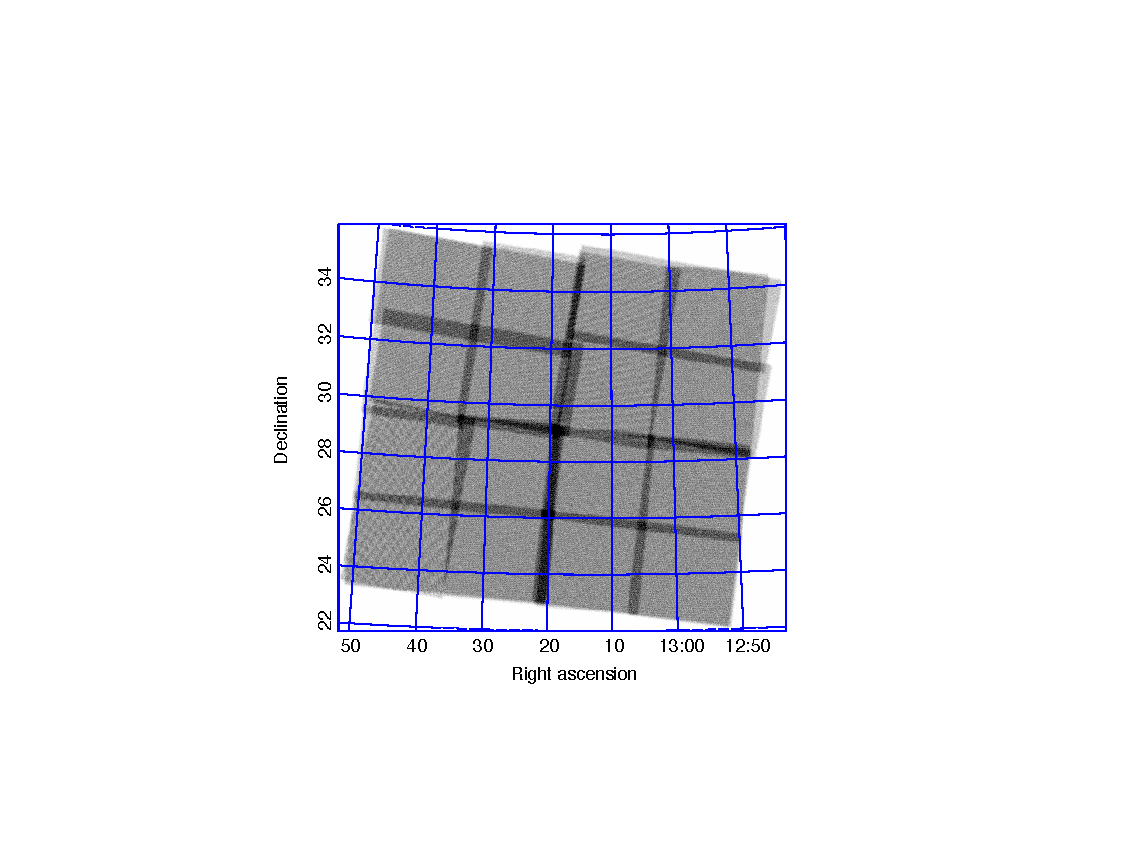
\includegraphics[scale=0.9, trim=0.0mm 5.0mm 0.0mm 0.0mm, clip=True]{ngpcoverage.pdf}
\caption{\protect\label{skymapn} The coverage map for 250\mic\ observations
of the NGP field.
The map shows the number of samples from the bolometer timelines contributing
to each map pixel, which ranges from 1 to 43, with the median value being 10.
The range of the grayscale is from 0 samples (white) to 27 samples
(black).}

\end{figure}

\begin{figure*} %2 
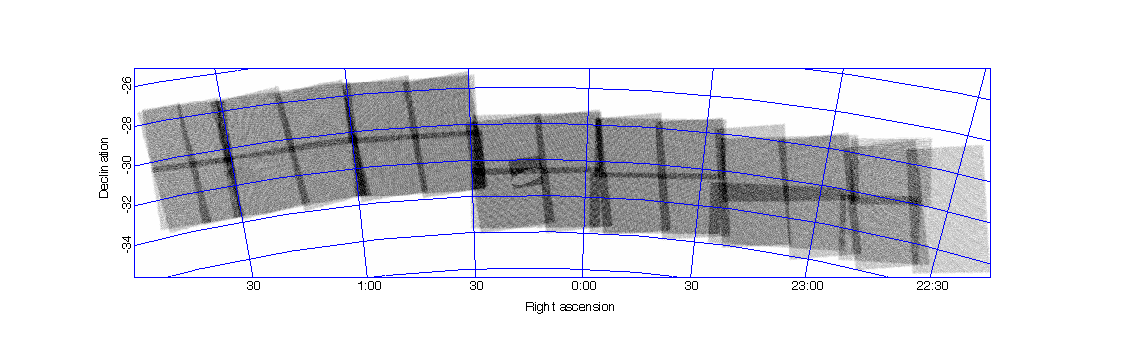
\includegraphics[scale=1., trim=0.0mm 5.0mm 0.0mm 5.0mm, clip=True]{sgpcoverage.pdf}
\caption{ \protect\label{skymaps} 
The coverage map for 250\mic\ observations
of the SGP field.
The map shows the number of samples from the bolometer timelines contributing
to each map pixel, which ranges from 1 to 36, with the median value being 9.
The range of the grayscale is from 0 samples (white) to 21 samples
(black).}
\end{figure*}

\section{Source detection} 

\subsection{The maps and background subtraction} 

A detailed description of the processing necessary to produce maps
from the {\it Herschel} raw data is presented in S17. The resulting 
maps have pixel sizes 3, 4, 6, 8 and 12 arc seconds for 100, 160, 250,
350 and 500 $\mu$m respectively. Note that these are different to the
canonical pixel sizes used for maps in the {\it Herschel} Science Archive,
which use 3.2, 3.2 6, 10 and 14 arc seconds respectively.  The maps
made with the PACS camera (100 and 160\mic, Poglitsch et al. 2010)
have units of Jy per pixel. The maps made with the SPIRE camera (250,
350 and 500\mic, Griffin et al. 2010) have units of Jy per beam.  The
beam areas at 250, 350 and 500\mic\ are 469, 831 and 1804 square arc
seconds, respectively (Valtchanov 2017).  The noise on the images is a
combination of instrumental noise and the confusion noise from sources
that are too faint to be detected individually.  S17 describes a
detailed analysis of the noise properties of the images.

Before attempting to detect sources in the maps, we first subtracted a
smoothly varying ``sky'' level to remove the foreground emission from
dust in our galaxy, so-called ``cirrus emission'', and also the
emission from clustered extragalactic sources fainter than our
detection limit. We used the {\tt nebuliser} function, a programme
produced by the Cambridge Astronomy Survey Unit to estimate and
subtract the sky level on astronomical
images\footnote{\url{http://casu.ast.cam.ac.uk/surveys-projects/software-release/background-filtering}}.

The choice of the filter scale used in {\tt nebuliser} is quite
critical, since it must be small enough for {\tt nebuliser} to remove
small-scale patches of cirrus emission but not so small that the flux
from large galaxies is reduced.  In practice, for the SPIRE maps we
found that a median filter scale of 30 pixels (3 arc minutes in the
250\mic\ band) followed by a linear filter scale of 15 pixels was an
acceptable combination.

We tested whether this filtering scale reduced the flux density of
extended extragalactic sources by creating simulated maps, placing
artificial extended sources on these maps, and then measuring the flux
densities of these sources after the application of {\tt nebuliser}.
Since the nearby galaxies detected by {\it Herschel} are mostly spiral
galaxies, we used exponential profiles for the artificial sources,
convolving these with the SPIRE point-spread function.  The
surface-brightness limit on photographic plates is typically
$\rm \mu_B \simeq 25\ mag\ arcsec^{-2}$, giving rise to the widely
used D25 optical diameters for galaxies.  Since these diameters are
roughly equivalent to a distance of five scale lengths from the centre
of a galaxy, we truncated the profiles of our artificial submillimetre
sources at five scale lengths, which gave us diameters, roughly
equivalent to D25 diameters in the optical waveband, which ranged from
24 to 192 arcsec.  The simulations showed that significant flux is
lost only for sources that have diameters larger than $~3$ arc
minutes, and even for sources above this size, the flux loss is
$\lesssim 10\%$. Note there are only 12 galaxies with diameter larger
than 3 arc minutes in the survey: 3 in the NGP and 9 in the SGP. 

We note that the application of {\tt nebuliser} will change the
clustering statistics of extragalactic sources.  Apart from the
foreground cirrus emission, {\tt nebuliser} removes the background
produced by the sources that are too faint to be detected
individually. This background varies because of the clustering of
these faint sources.  A source catalogue made without any background
subtraction will include more sources where this background is high as
a result of clusters of these faint sources, and so the clustering of
the sources in this catalogue will be stronger than in a catalogue
produced from an image in which this background emission has been
removed. An investigation of the clustering in the H-ATLAS catalogues,
which includes an analysis of the effect of the subtraction of this
background, will be presented by Amvrosiadis et al. (in preparation).

For the PACS maps, the $1/f$-noise from the instrument is much larger than
for SPIRE, making the foreground cirrus emission and the background
emission from faint galaxies difficult to detect. Since we could not
clearly detect the foreground/background emission on smaller
scales, we used a {\tt nebuliser} scale of 5 arcminutes.

The raw maps from the SPIRE pipeline have a mean of zero, but the
output maps from {\tt nebuliser} have a modal pixel value that is
zero. For the SPIRE bands, the instrumental noise is low enough that
the flux distribution of detected sources skews the pixel distribution
to positive values so the mean is slightly positive (1.0, 1.0 and 0.6
mJy/beam at 250, 350 and 500\mic).  The PACS detector is less
sensitive and less stable than SPIRE, and so the instrumental noise
dominates over the confusion noise and the pixel distribution is close
to Gaussian; the mean of the {\tt nebulised} PACS maps are very close
to zero (0.016\,MJy\,sr$^{-1}$, for both the 100 and 160\mic\ maps).

\subsection{Source Detection} 


In this section we describe the method used to find the
sources on the images. Additional details are given in V16.
Sources were detected using the {\tt MADX} algorithm (Maddox et al in prep)
applied to the SPIRE maps.  {\tt MADX} creates maps of the signal-to-noise
ratio and identifies sources by finding peaks in the signal to noise. The
detection and measurement of fluxes is optimised by using a matched
filter that is applied to both the signal map and the noise map. 

The SPIRE instrumental noise maps are created from the number of
detector passes and the estimated instrumental noise per pass,
$\sigma_{\mathrm{inst}} /\sqrt{N_ {\mathrm{sample}}}$, as described in S17 and V16.

%% the 2.5sig cut is instrumental only the 4 sigma includes both inst
%% and confusion
%% flux in other bands measured at optimal position, as defined from
%% the 250micron maps; there is a clean process for each band
%% individually
 
Since the noise consists of both instumental noise and
confusion noise from the background of undetected sources, we follow
the approach of Chapin et al (2011) to calculate the optimal matched
filter in each of the three SPIRE bands. Details of estimation and
form of the matched filter are discussed in V16.  The resulting
matched filters are slightly more compact than the corresponding PSFs,
and have slightly negative regions outside the FWHM.  

In the first step of the source detection, peak pixels which have
values $>2.5\sigma$ in the filtered 250-\micron\ map are considered as
potential sources.  We use the 250-\micron\ map since most sources have
the highest signal-to-noise in this map.  The source position is
determined by fitting a Gaussian to the flux densities in the pixels
surrouding the pixel containing the peak emission.  As an initial
estimate of the flux density of the source in each SPIRE band, {\tt MADX}
takes the flux density in the pixel closest to the 250-$\mu$m
position.

The high source density on the SPIRE maps means that these flux
estimates often contain contributions from neighbouring sources.  To
mitigate this effect, {\tt MADX} uses the following procedure.  In each
band, {\tt MADX} sorts the sources in order of decreasing flux density.  The
flux density of the brightest source is then more precisely estimated
using the value of the filtered map interpolated to the exact
(sub-pixel) position from the 250-\micron\ map.  Using this flux
estimate, a point source profile is then subtracted from the map at
this position. Since the bright source is now removed from the map,
any fainter sources nearby should have fluxes that are not
contaminated by the brighter source. The program then moves to the
next brightest source and follows the same set of steps.  One
consequence of these steps is that some sources will now have
250-$\mu$m flux densities less than the original $2.5\sigma$ cut.
Since most sources are brighter at 250$\mu$m than at the two longer
wavelengths, the estimates of the flux densities in the 350-$\micron$\ and
500-$\micron$\ bands are on average significantly lower in signal to noise,
and can even sometimes be negative. We retain these negative
measurements so that the  distribution of fluxes in the
catalogues is consistent with the errors, and not truncated at an
arbitrary limit. 

\begin{figure*} %3
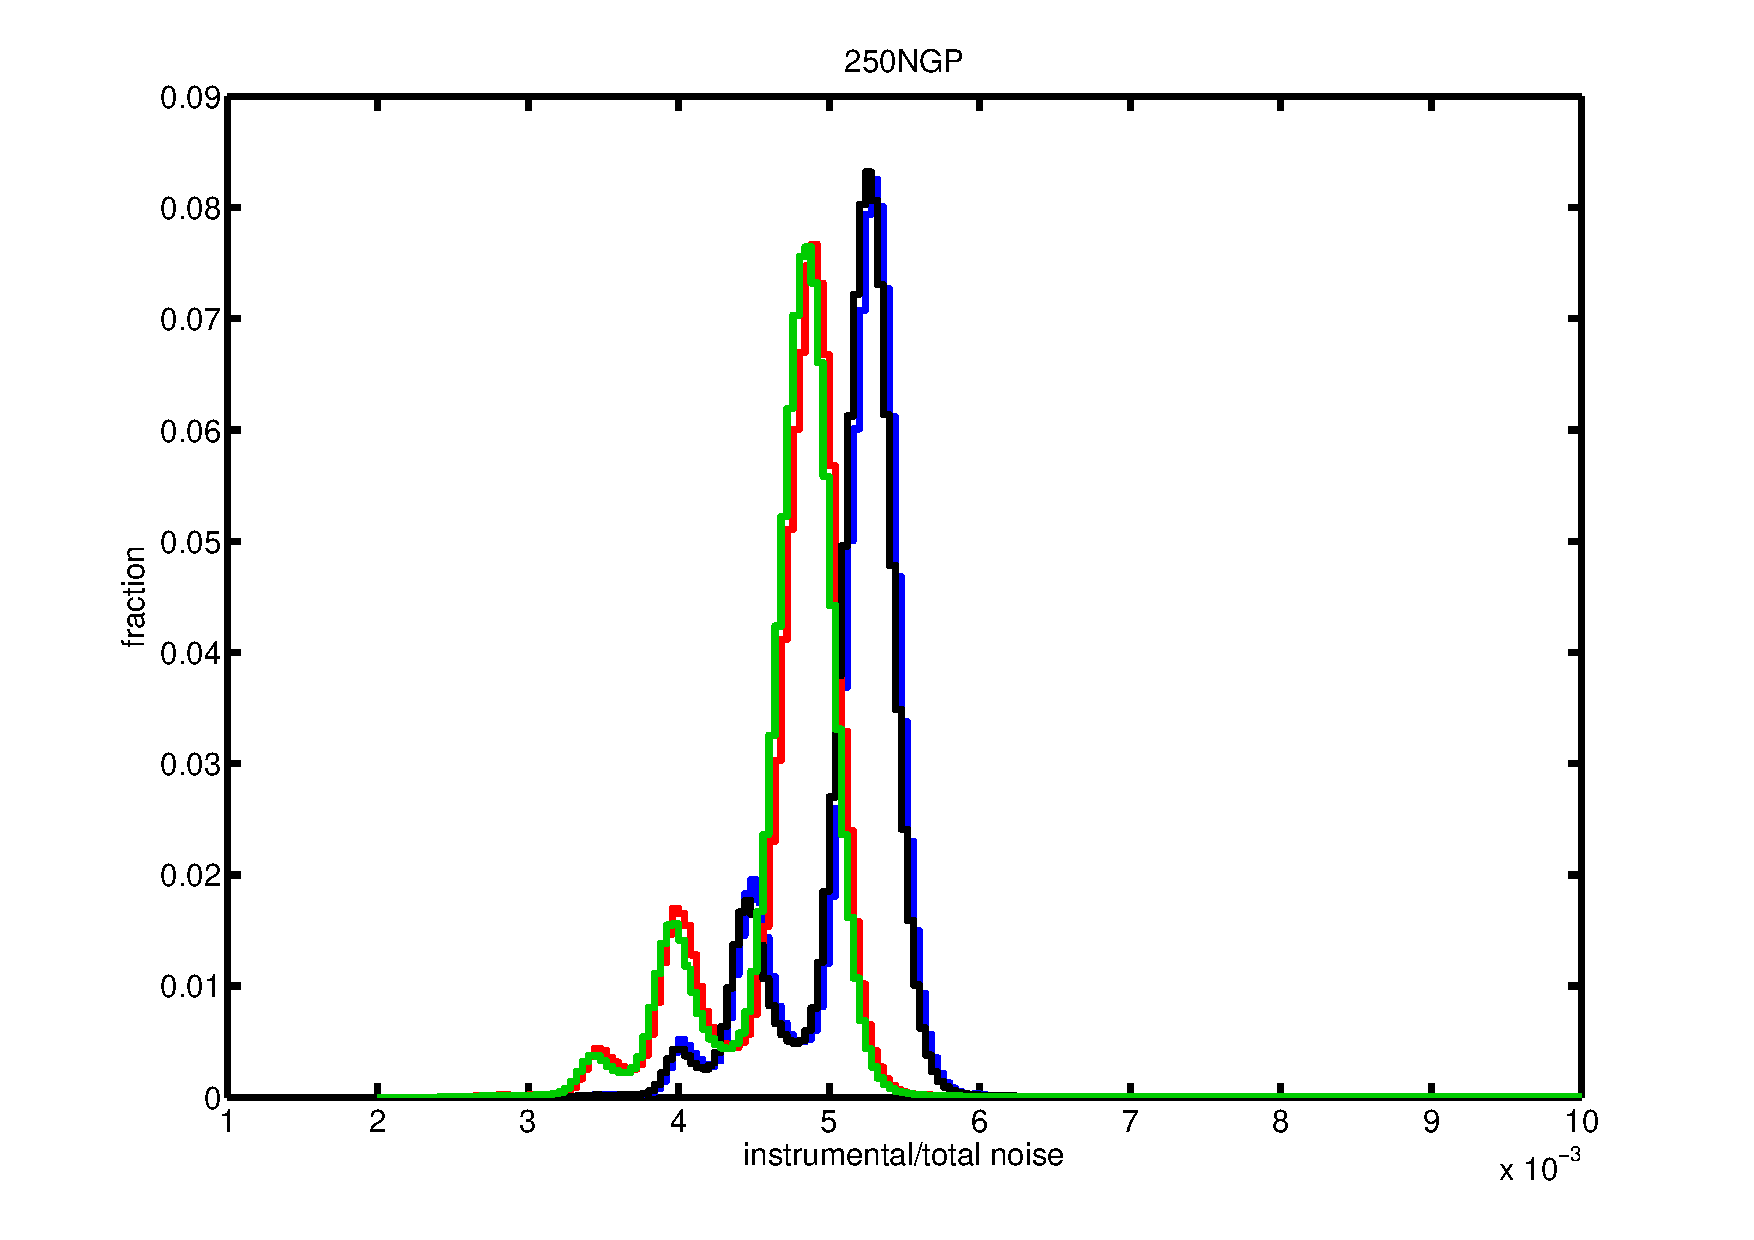
\includegraphics[width=0.3\textwidth]{flux_noise_250NGP.pdf}
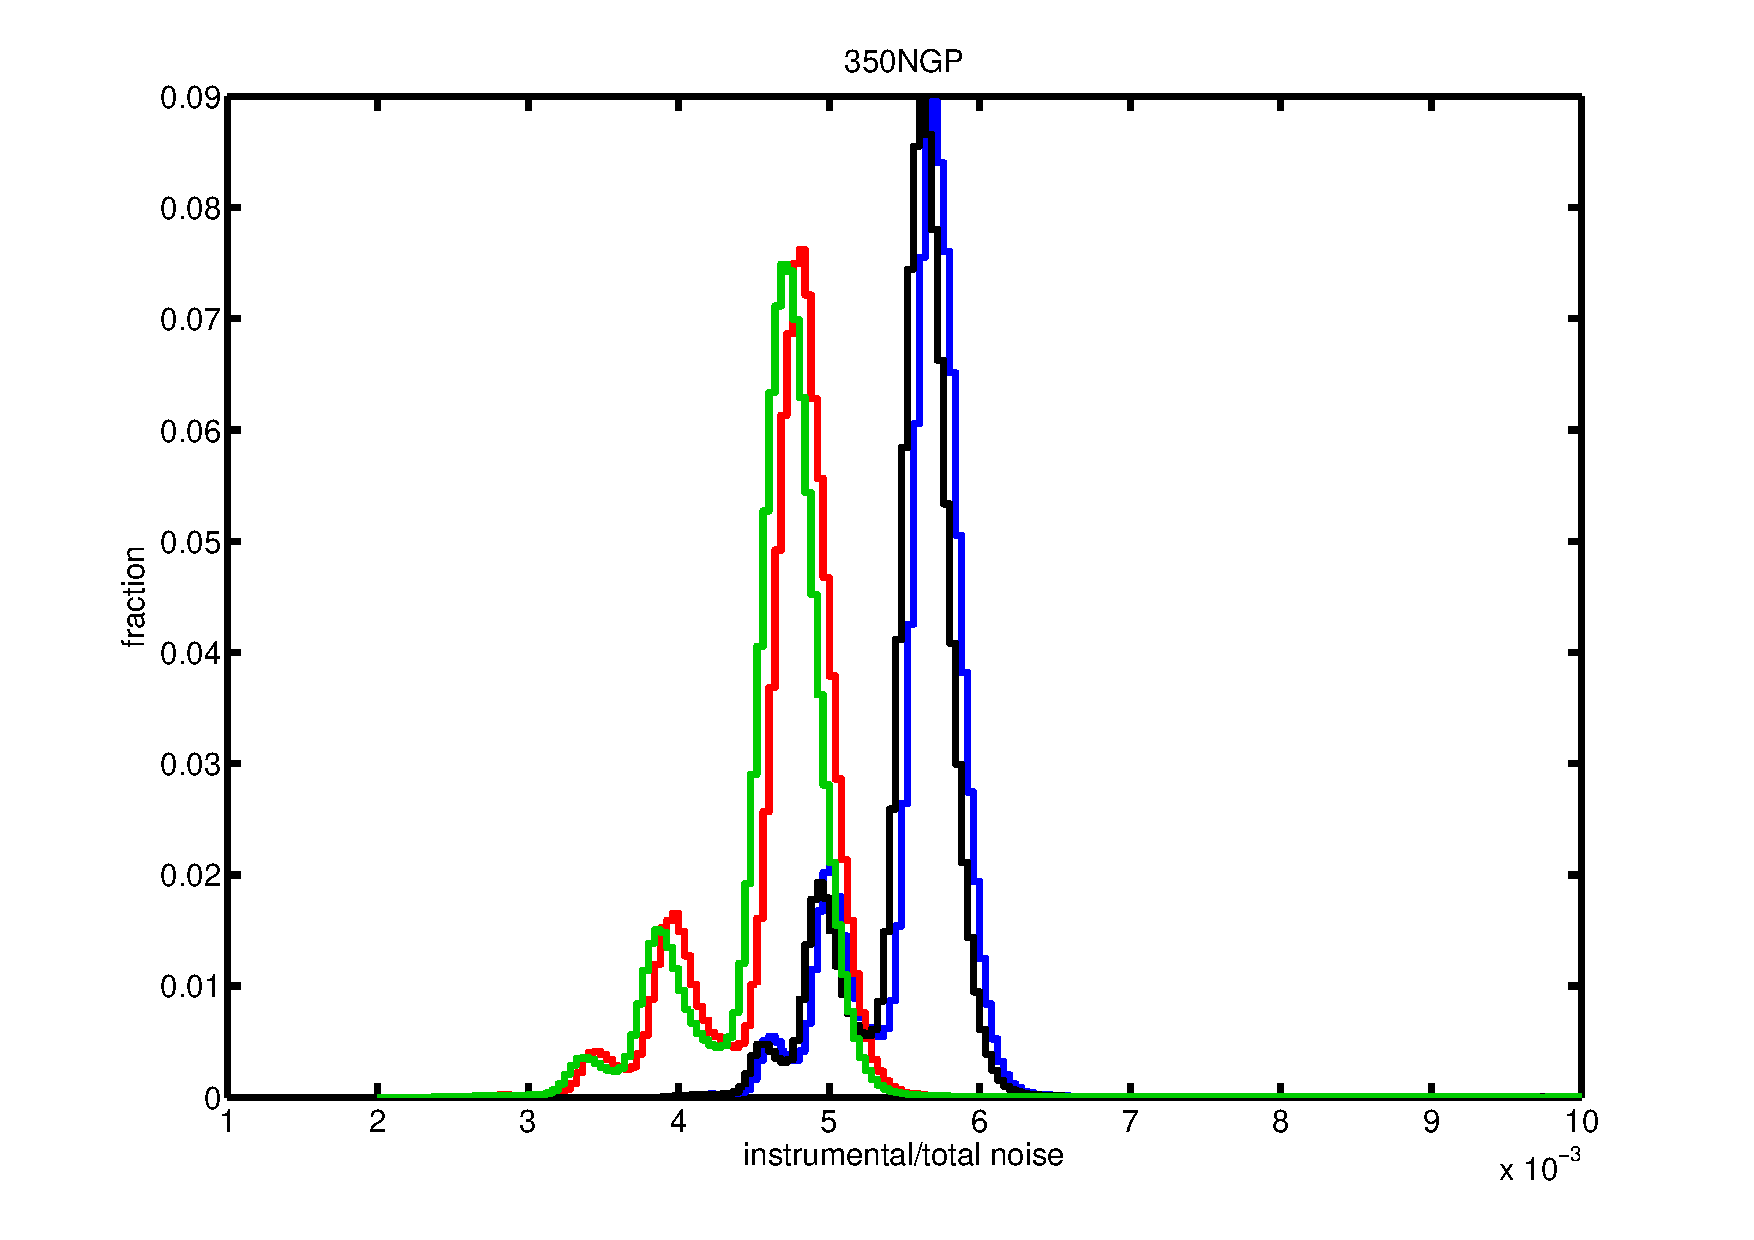
\includegraphics[width=0.3\textwidth]{flux_noise_350NGP.pdf}
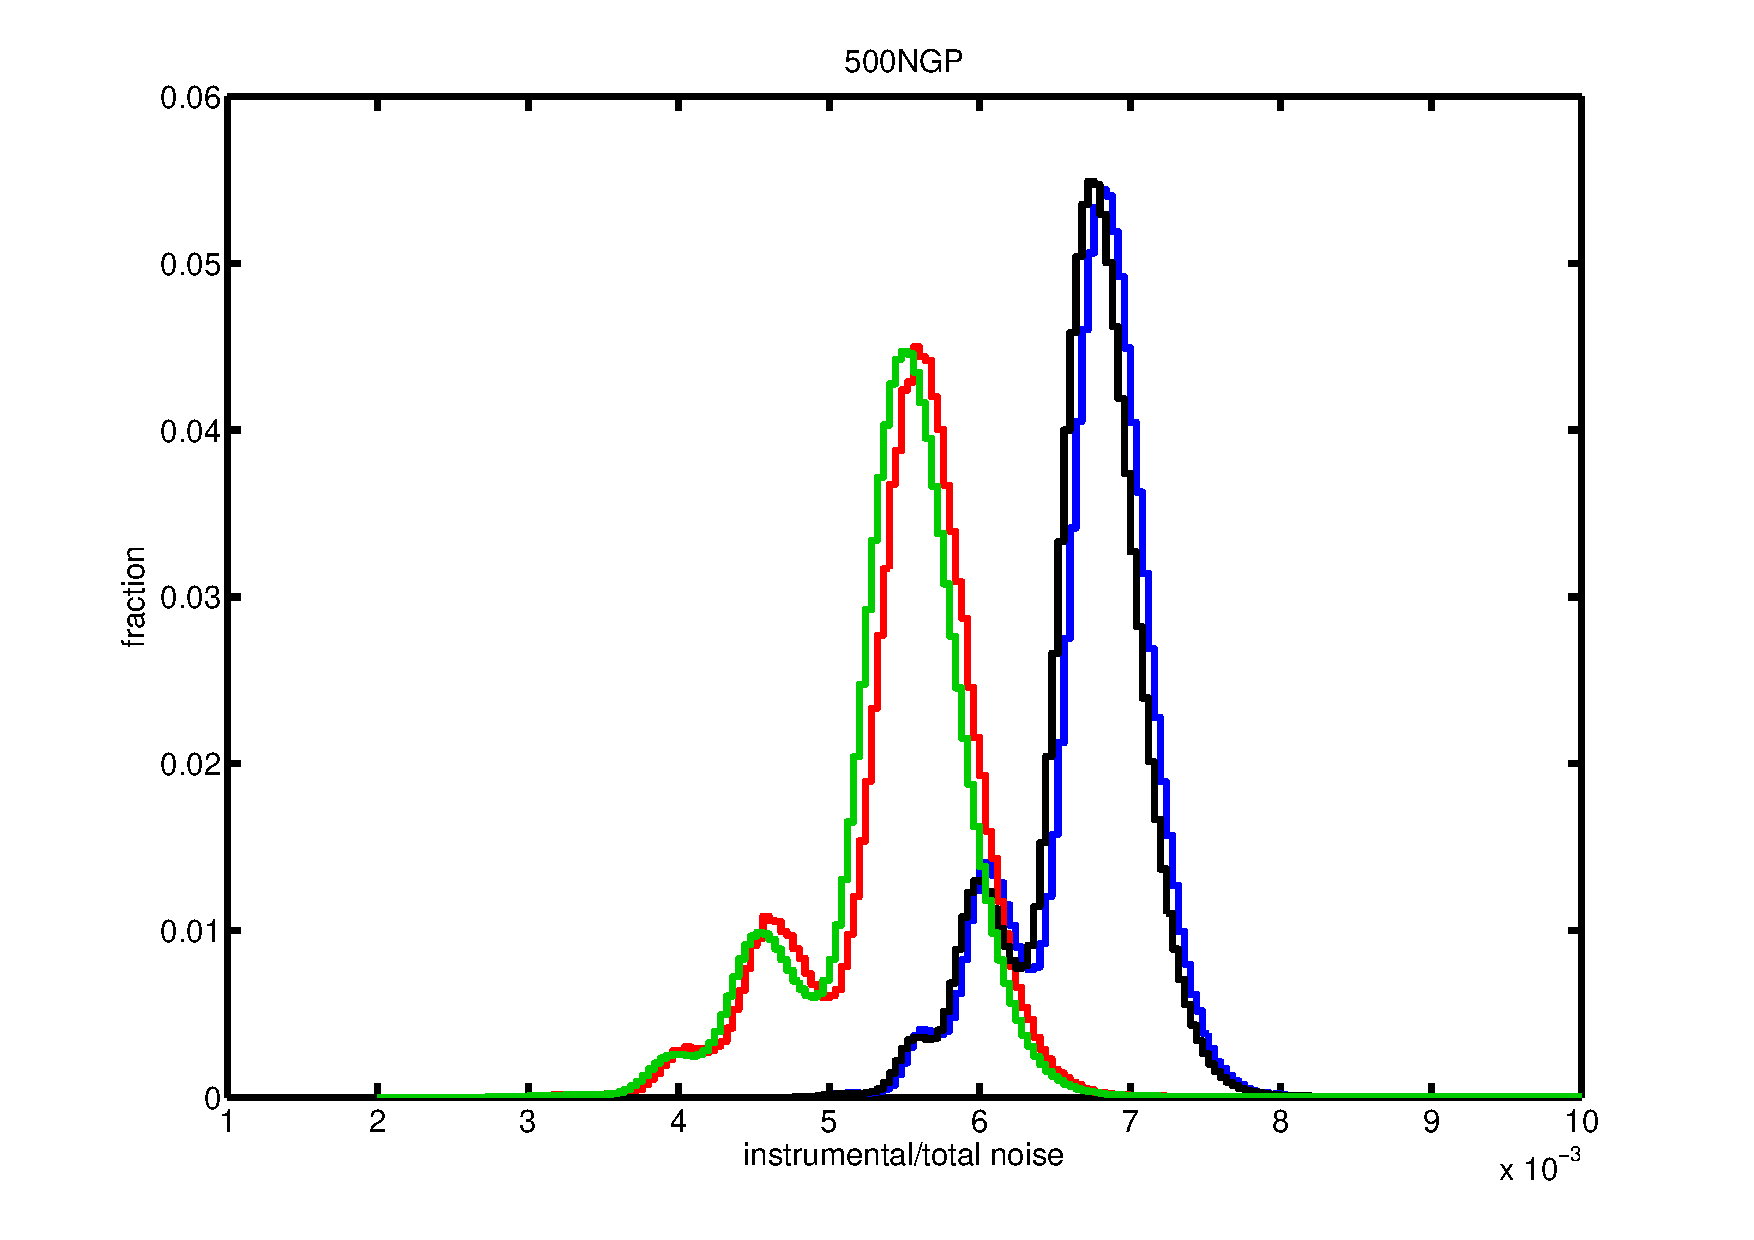
\includegraphics[width=0.3\textwidth]{flux_noise_500NGP.pdf}
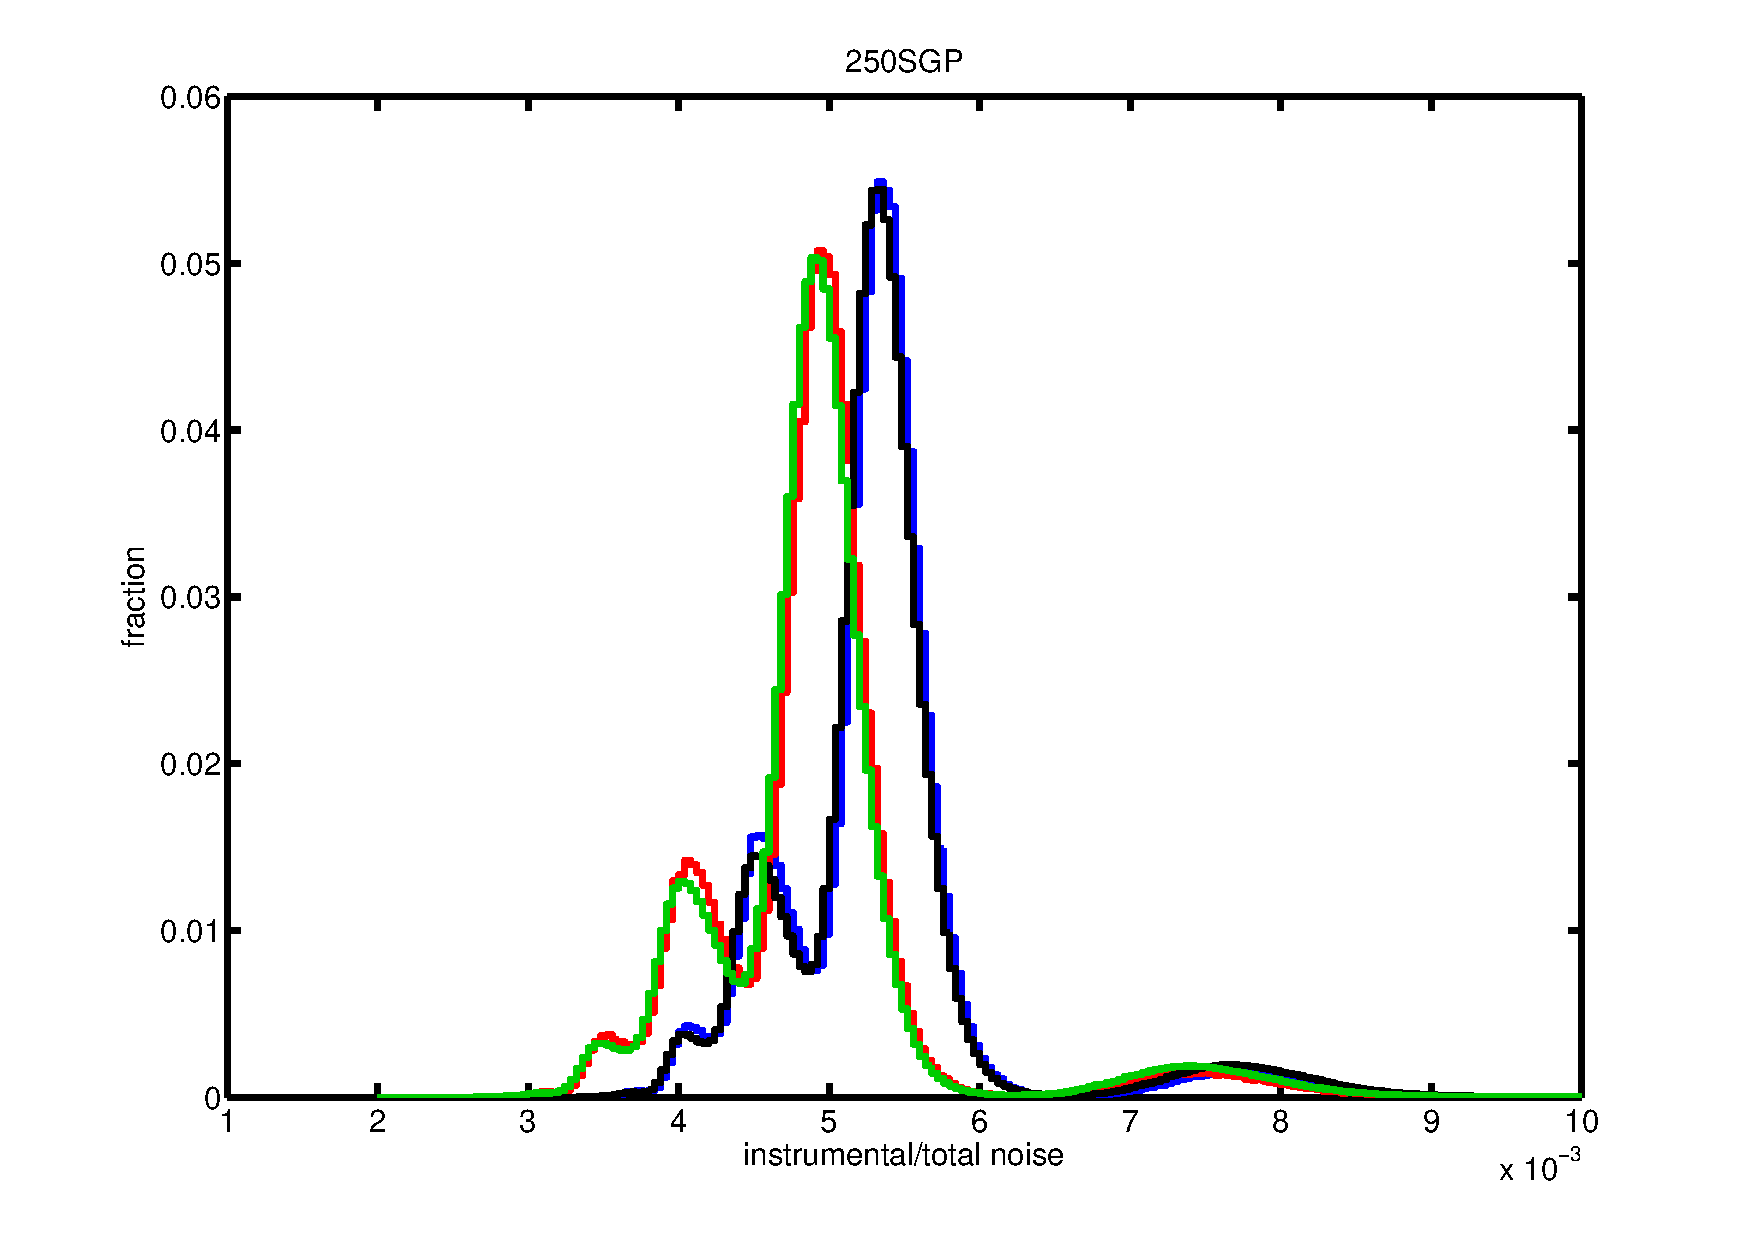
\includegraphics[width=0.3\textwidth]{flux_noise_250SGP.pdf}
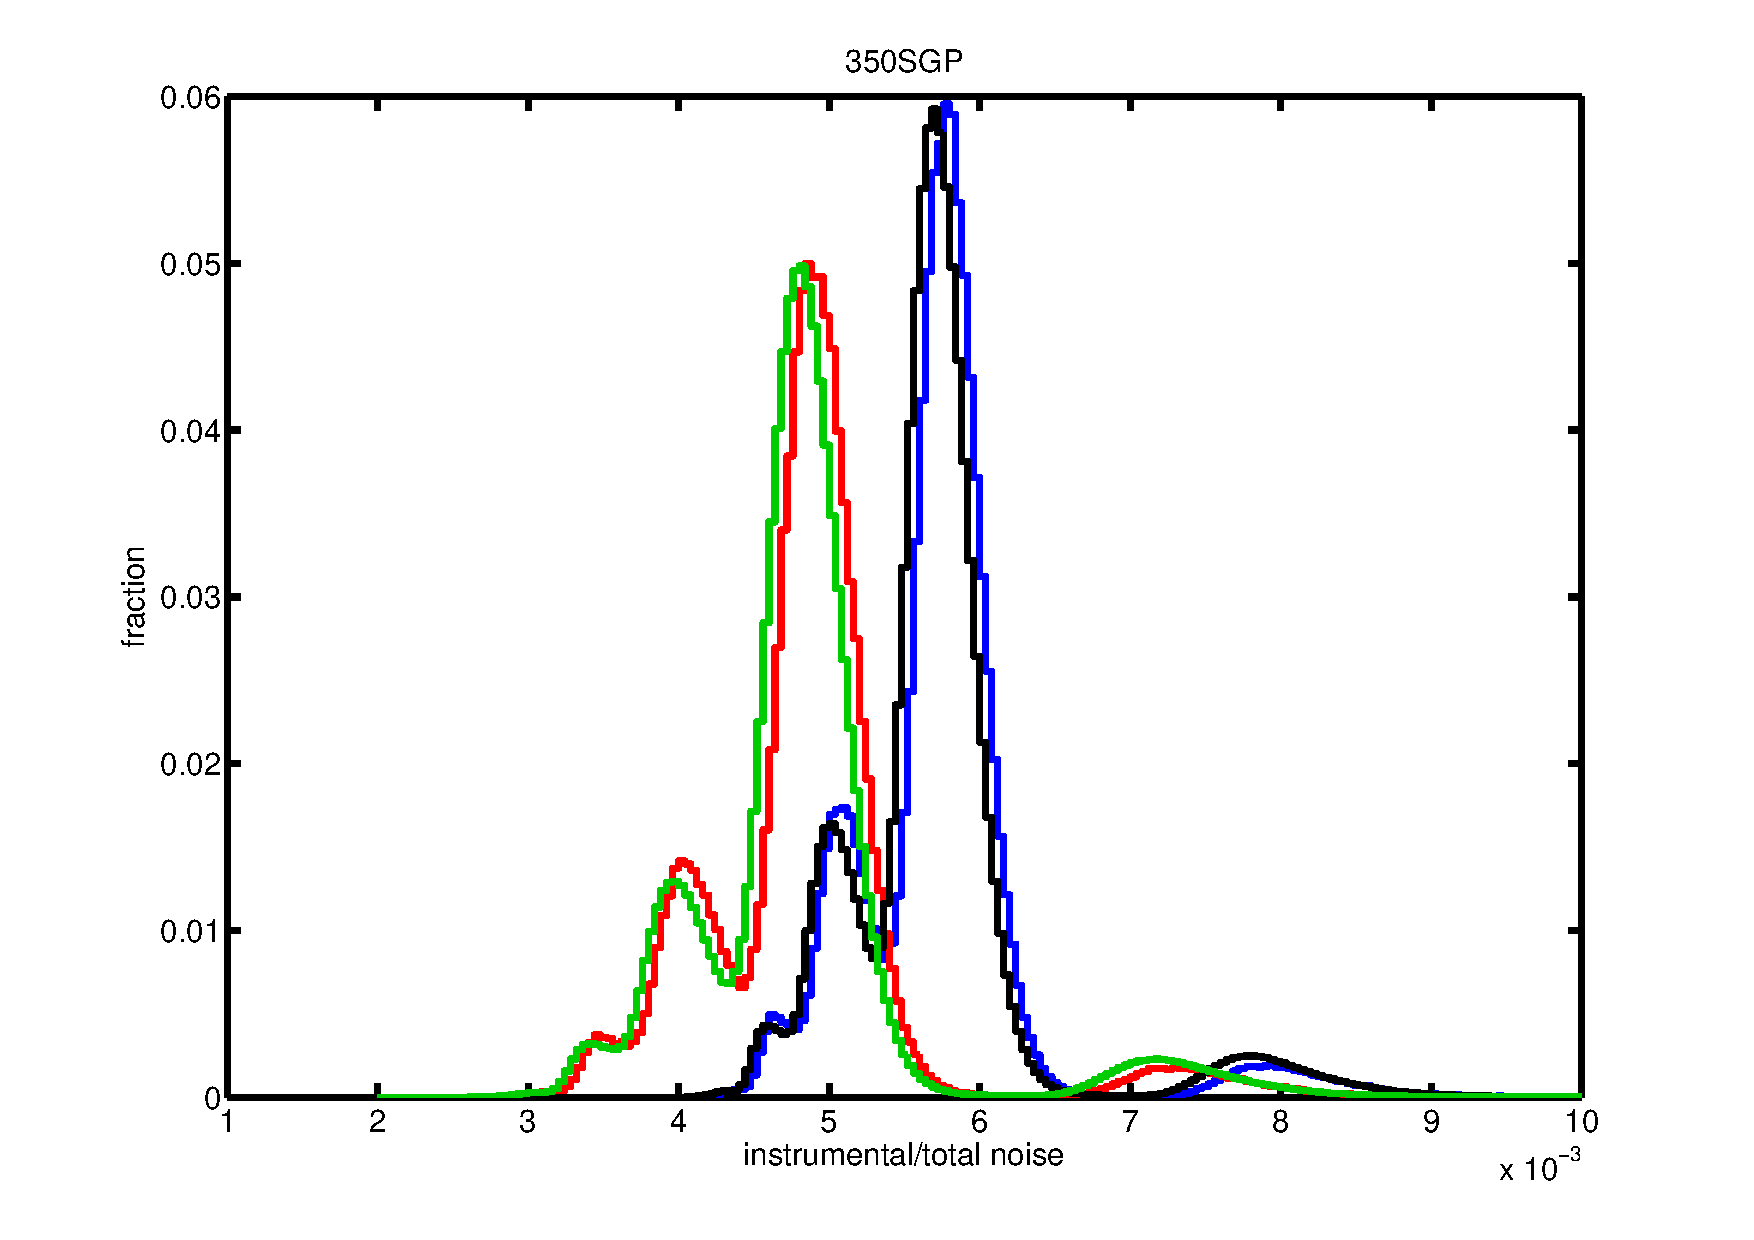
\includegraphics[width=0.3\textwidth]{flux_noise_350SGP.pdf}
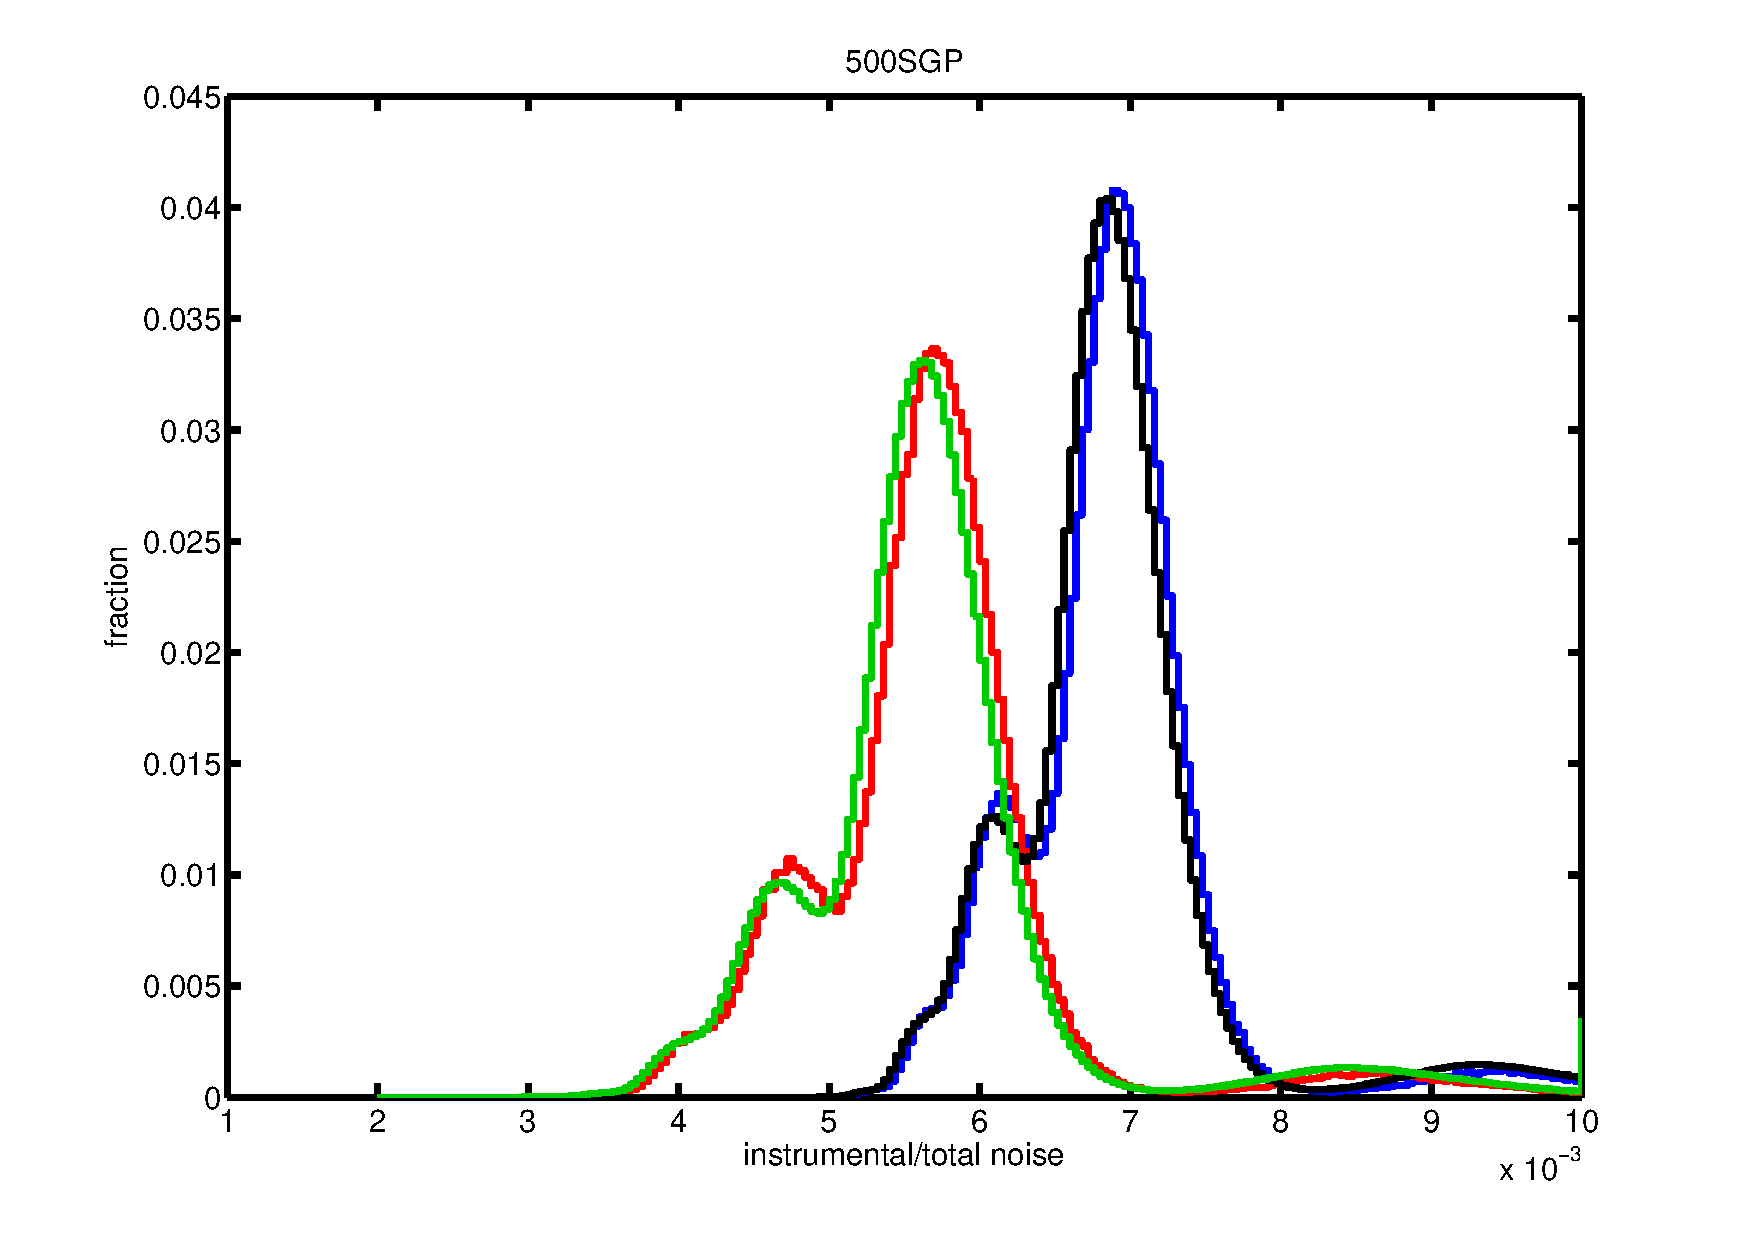
\includegraphics[width=0.3\textwidth]{flux_noise_500SGP.pdf}
\caption{The distribution of instrumental and total noise for the
  250-\micron, 350-\micron\ and 500-\micron\  bands for the NGP and SGP
  fields.  Green shows the instrumental noise and black the total
  noise for all pixels; red shows the instrumental noise and blue the
  total noise at the positions of all sources.  The multiple peaks are
  the results of our tiling strategy. The main peak corresponds to the
  large fraction of the survey area that was covered by two individual
  {\it Herschel} observations (S17). The smaller peaks correspond to
  the small fraction of the survey area that was either covered by
  more than two observations or, in the case of one end of the SGP
  (S17), a single observation (the small peak at the right in the
  bottom panels.}
\label{fig_noise}
\end{figure*}

\begin{figure} %4
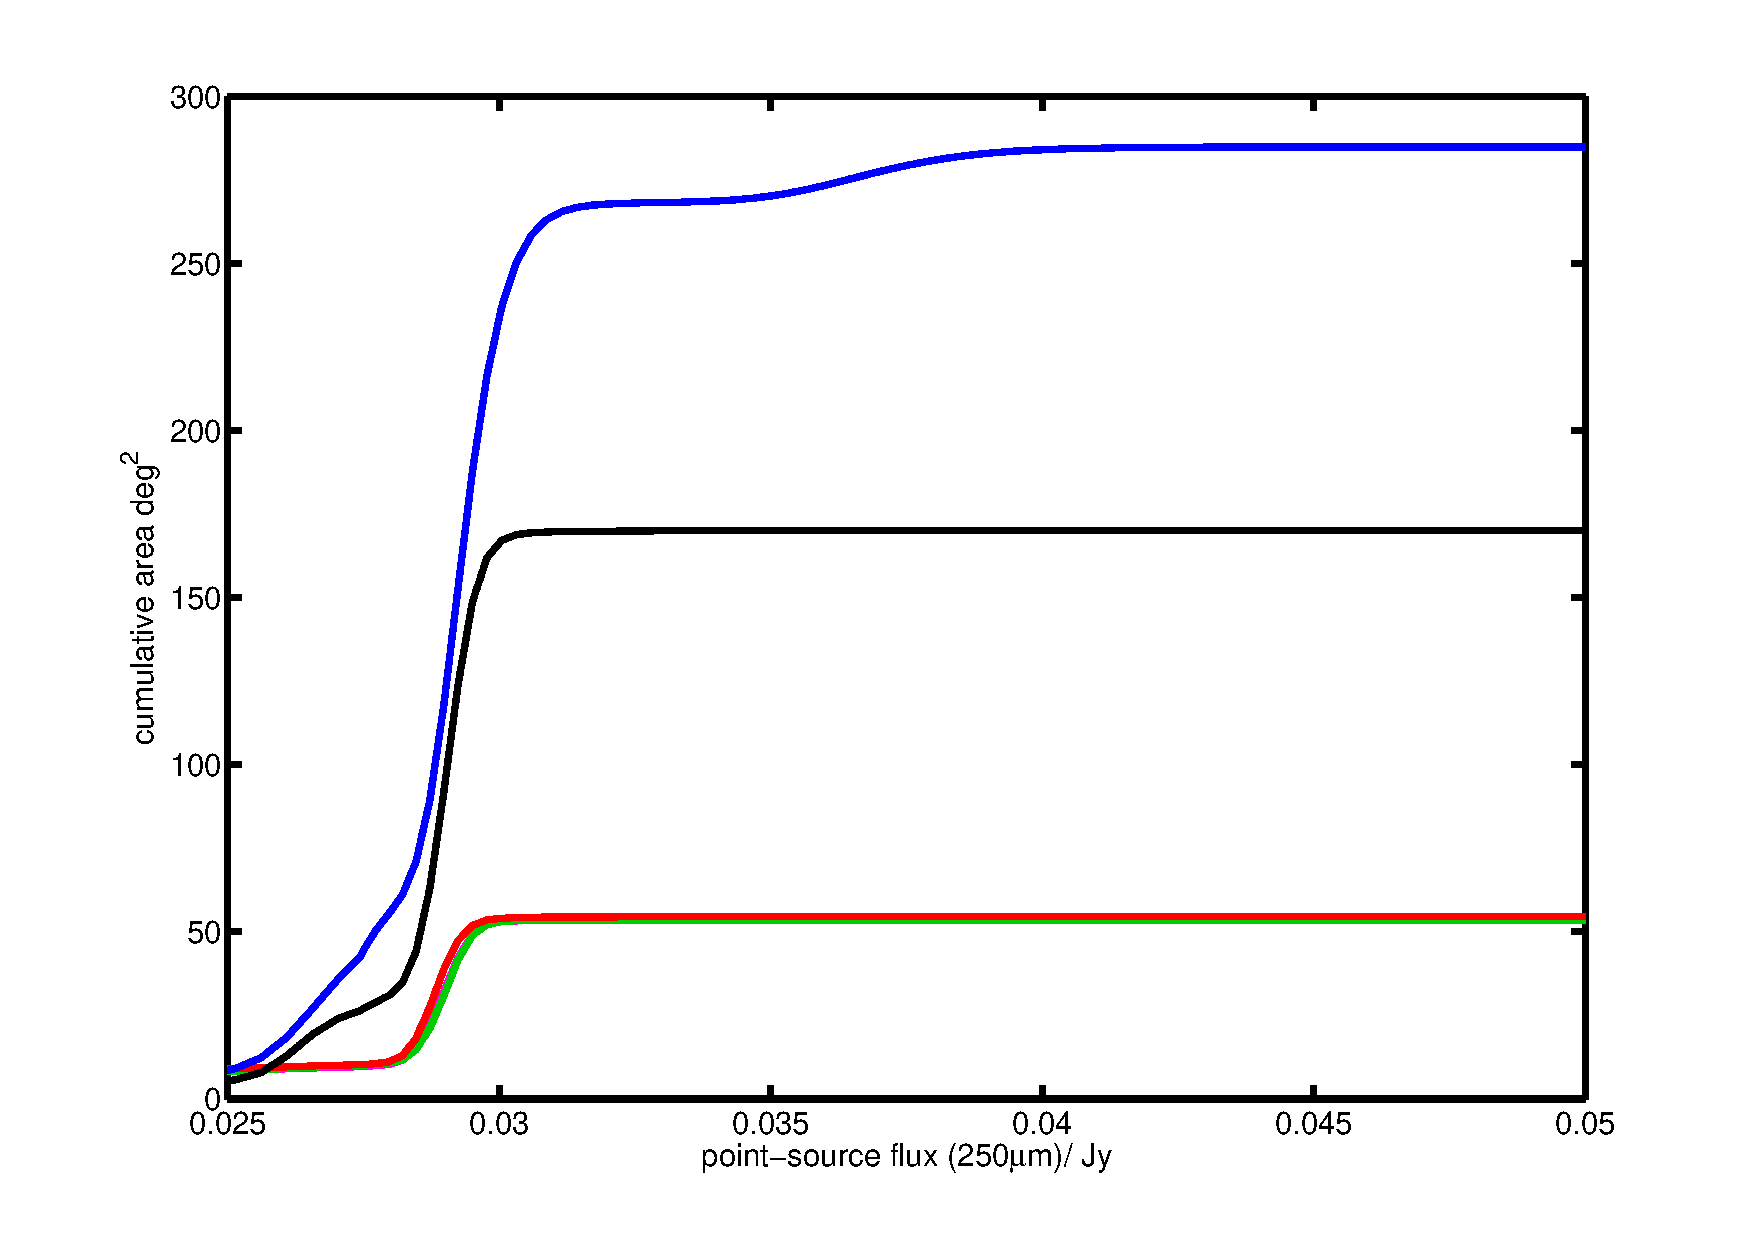
\includegraphics[width=0.5\textwidth]{flux_area_250.pdf}
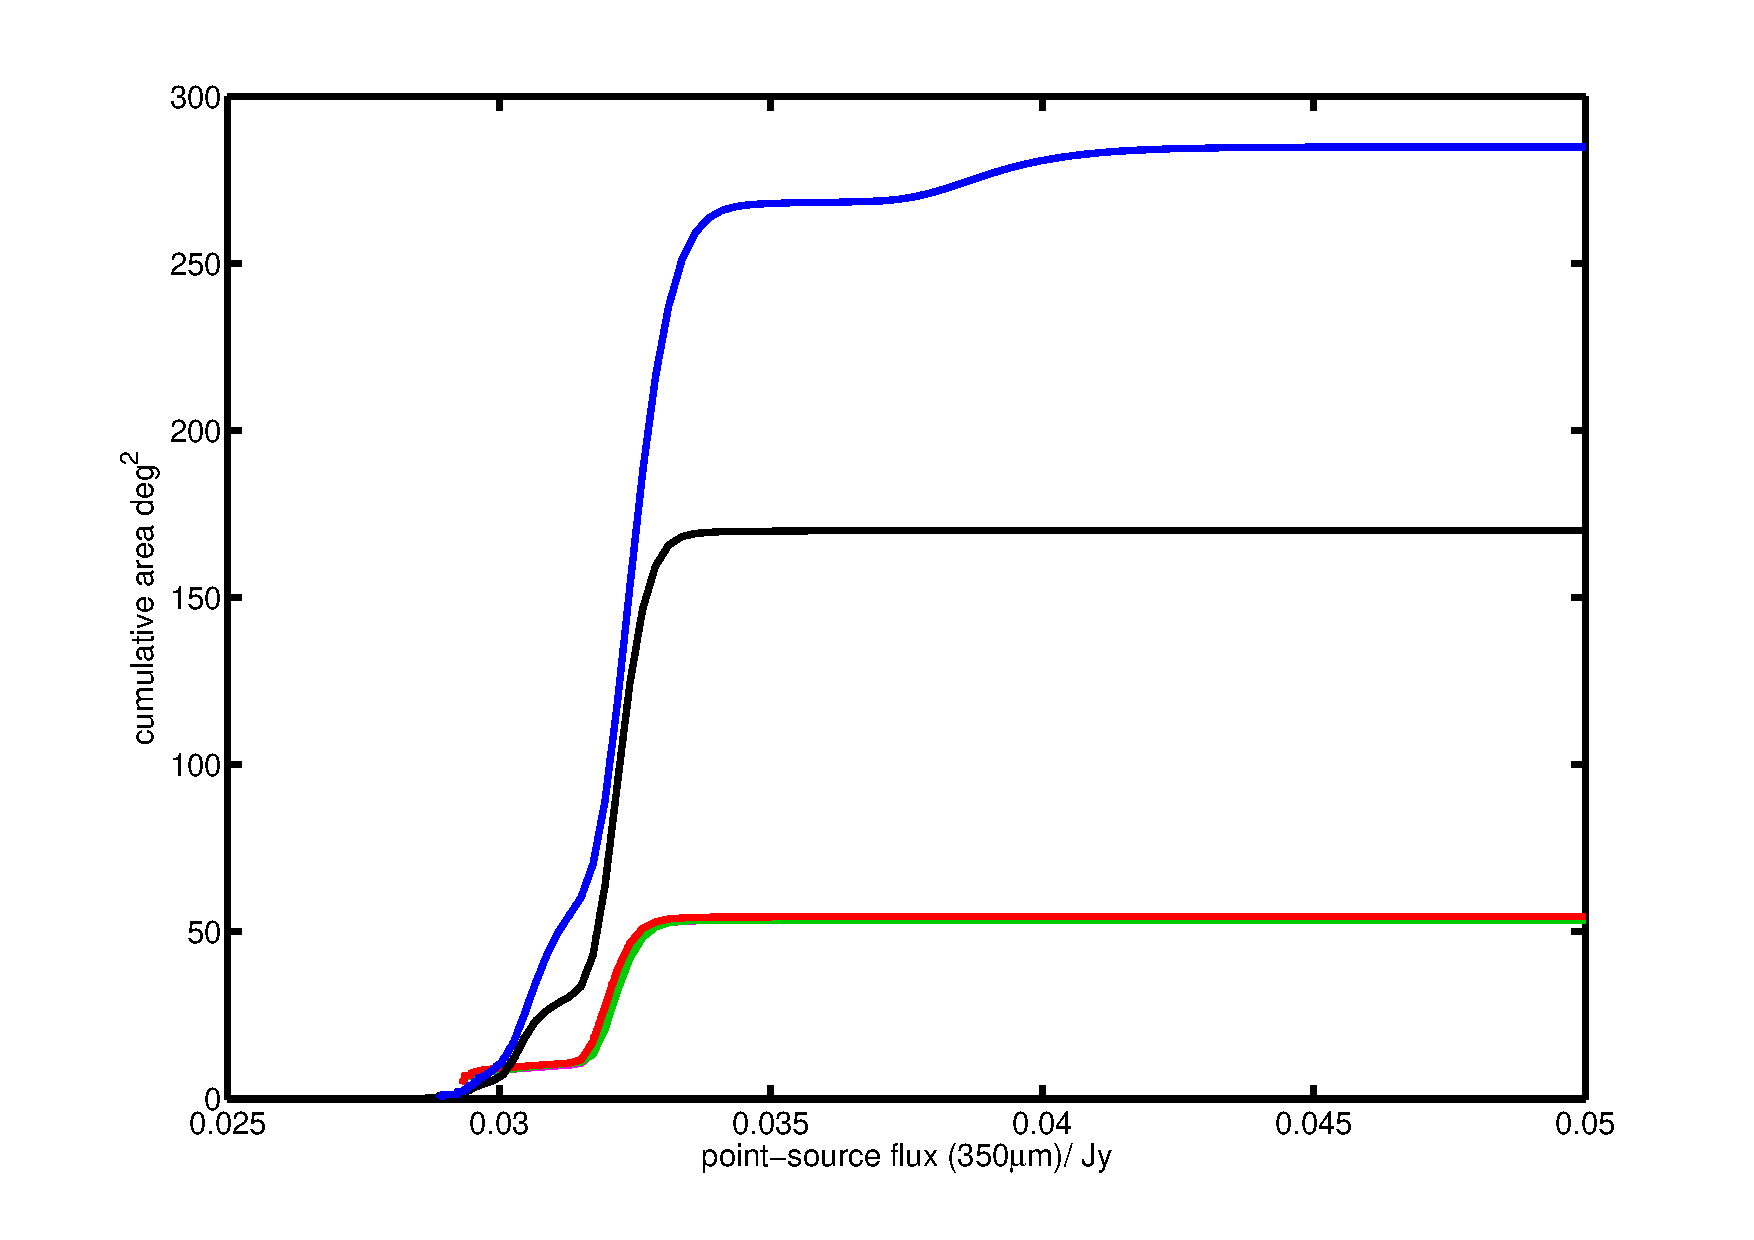
\includegraphics[width=0.5\textwidth]{flux_area_350.pdf}
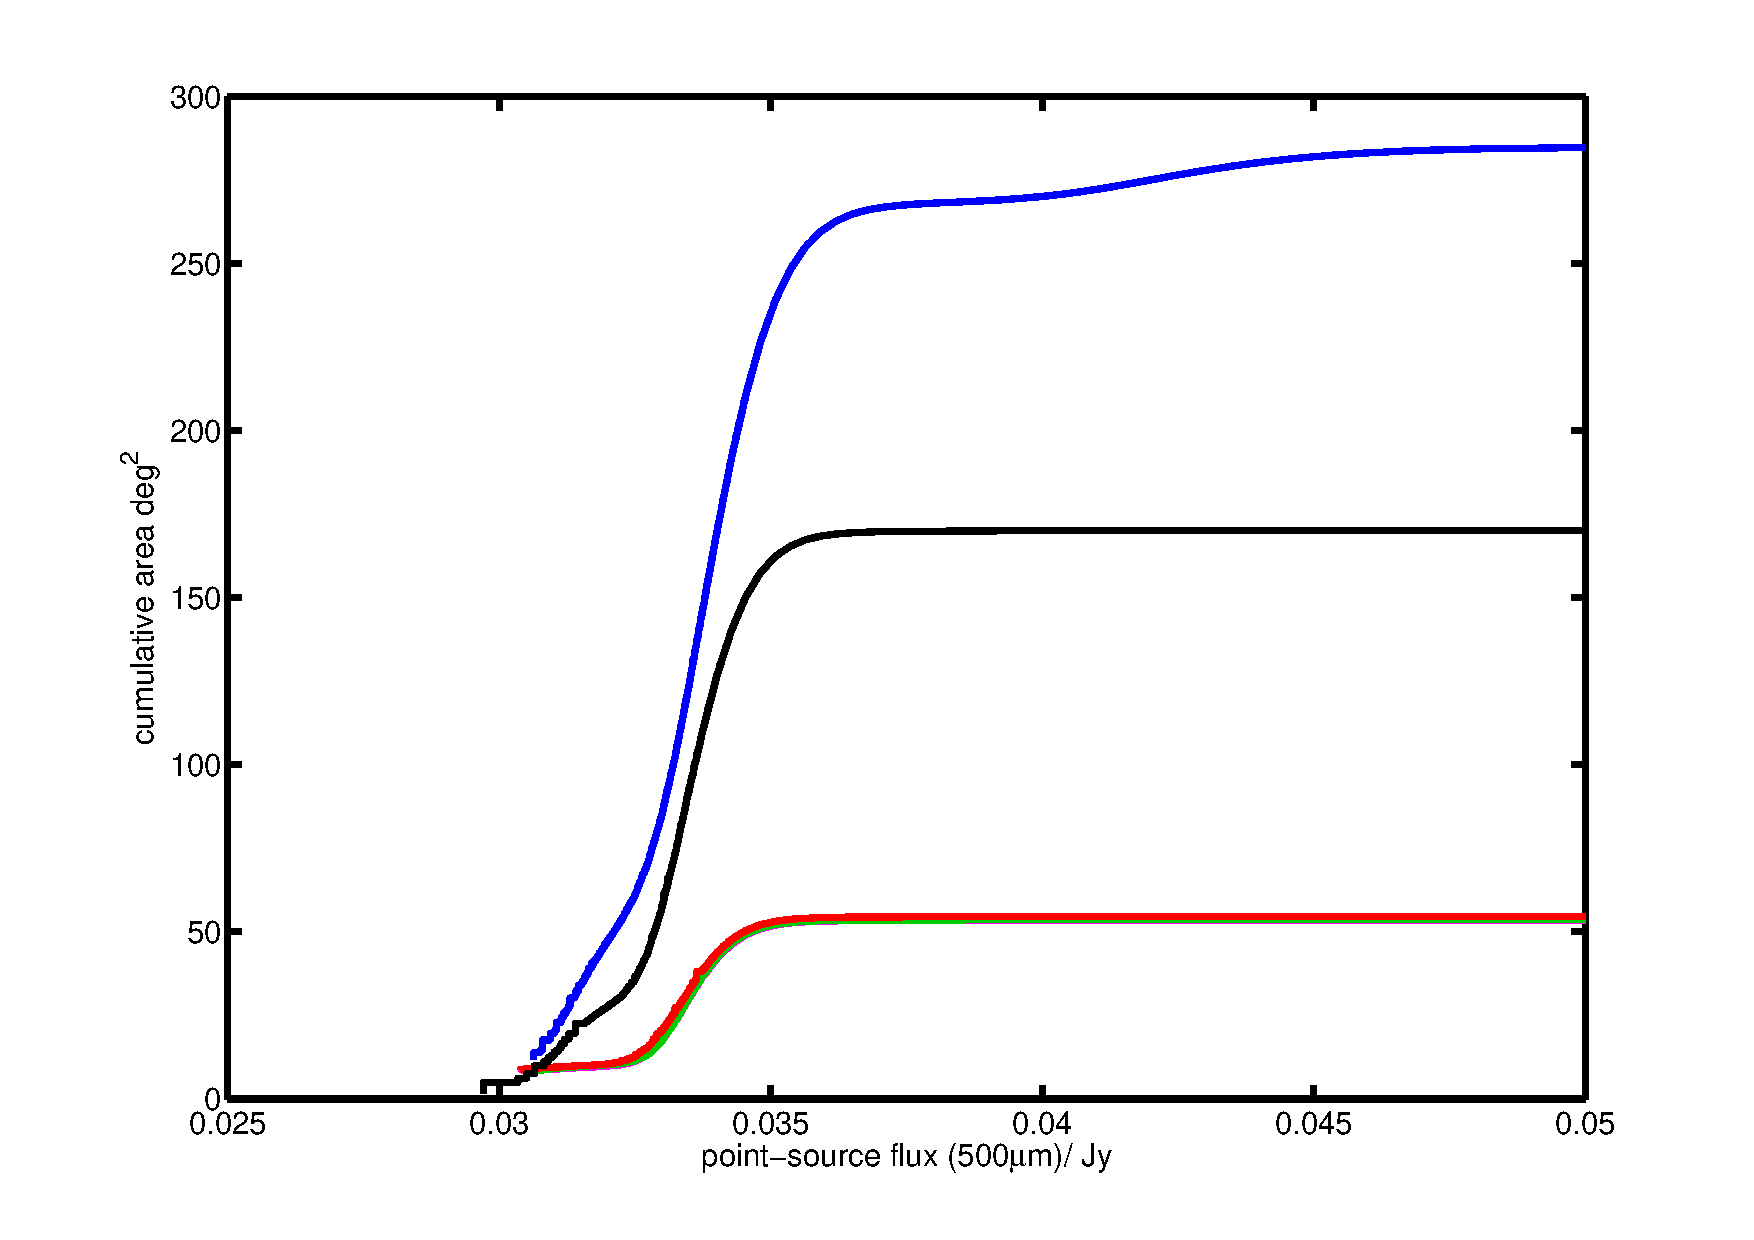
\includegraphics[width=0.5\textwidth]{flux_area_500.pdf}
\caption{The relationship between area and 4$\sigma$ flux-density
  limit for the H-ATLAS fields: NGP - black; SGP - blue; GAMA9 -
  magenta; GAMA12 - green and  GAMA15 - cyan.  The more sensitive areas
  correspond to the tile overlaps in each field.  The westerly end of
  SGP has only a single SPIRE observation, which explains the kink at
  high flux densities in the blue line in these panels.}

\label{fig_areas}
\end{figure}

\section{Photometry}

\subsection{Point sources}

\subsubsection{SPIRE}

V16 carried out extensive simulations to determine the
errors on the flux density estimates for point sources.
They followed the simple procedure of injecting artificial
sources of known flux density into the real maps and then
using {\tt MADX} to estimate their flux densities
(Section 2.2).  
They found that at 250\mic, the detection
wavelength, the confusion noise varies as a function
of source flux and gave a simple formula to approximate this:
\smallskip
\begin{equation}
\sigma_{\mathrm{con}250} = \sqrt{\min(0.0049,f_{250}/5.6)^2 +
  0.00253^2} \ \ \mathrm{Jy}.
\end{equation}
\smallskip
\noindent They found that 
at 350\mic\ and 500\mic\ the confusion noise 
is roughly constant, with $\sigma_{\mathrm{con}350} = 0.00659$~Jy and
$\sigma_{\mathrm{con}500} = 0.00662$~Jy.

We calculated the errors in the flux density estimates for each
individual source, using these formulae to estimate the confusion
noise and the maps of the instrumental noise (Section 2.2) to estimate
the instrumental noise, then adding the confusion and instrumental
noise in quadrature.


Our strategy of creating the H-ATLAS survey from overlapping tiles
(S17) means that the instrumental noise varies systematically between
different areas of the maps.  Figure~\ref{fig_noise} shows histograms
of instrumental noise and total noise (instrumental noise plus
confusion noise) for all pixels and at the positions of all sources.
The multiple peaks are the results of our tiling strategy. The main
peak corresponds to the large fraction of the survey area that was
covered by two individual {\it Herschel} observations (S17). The
smaller peaks at lower noise correspond to the smaller fraction of the
survey area that was covered by more than two observations. The small
peak at higher noise in the SGP field corresponds to the area at the
western end that was covered by a single observation (S17).

The variation of noise across the maps means that the 4$\sigma$
flux-density limit varies over the fields, and hence the available
area depends on the chosen flux limit. Figure~\ref{fig_areas}
shows the relationship between area and flux-density limit for each of
the H-ATLAS fields, including the GAMA fields.



\subsubsection{PACS}

As in V16, we used aperture photometry to estimate the flux densities
in the two PACS bands. We did this for two reasons. First, the PACS
PSF for our observing mode (fast-parallel scan mode) is not well
determined near its peak (see V16 for an extensive
discussion). Second, if we estimated the 100- and 160-$\micron$ flux
densities at the 250-$\mu$m position, as we did for the 350- and
500-$\mu$m bands, we would be likely to significantly underestimate
the flux density because of the higher resolution of the PACS maps.

V16 describes an extensive investigation of the optimum aperture size,
and we follow that paper in using an aperture with a radius equal to
the FWHM, which is 11.4 arc seconds for 100\mic\ and 13.7 arc seconds
for 160\mic. Since the ``sky'' level has already been subtracted with
{\tt nebuliser}, we made no correction for any residual sky level.  To
provide an accurate treatment of the contribution from fractional
pixels near aperture boundaries, we divided each pixel into 16, and
assigned one sixteenth of the flux density in each sub-pixel,
corresponding to a nearest-pixel interpolation. Then the flux density
from each sub-pixel that lies within the aperture is added together to
produce the total aperture flux.  We also tried bilinear, and bicubic
interpolation methods and found negligible differences in the
resulting aperture fluxes.  Since only $\simeq$10\% of the SPIRE
sources were clearly detected on the PACS images, we centred the
aperture on the 250-$\mu$m position.

We corrected the aperture flux densities to total flux densities using
the table of the encircled energy fraction (EEF) described in V16 and
available at \url{http://www.h-atlas.org/}.  We made a further
correction to allow for the effect of the errors on the 250-$\micron$
positions, since any error in the position will lead to the small PACS
apertures missing flux. V16 describes simulations of this effect, and
we follow that paper in compensating for this effect by multiplying
the flux densities by 1.1 and 1.05 at 100 and 160 $\mu$m,
respectively.

We describe how we estimated the errors on these flux estimates in the
following subsection.

\subsection{Extended sources} 

The approach in Section 3.1 gives optimal flux density estimates for
point sources, but will substantially underestimate the flux density
of extended sources.  As in V16, we used the $r-$band sizes of optical
counterparts to the {\it Herschel} sources to indicate which sources
are likely to require aperture photometry rather than the methods
described in the last section.  We followed different methods for the
NGP and the SGP because of the lack of a comprehensive identification
analysis for the SGP. We estimate aperture photometry for extended
source in both PACS and SPIRE bands.

\subsubsection{The NGP}

In the NGP, F17 carried out a search for optical counterparts to the
{\it Herschel} sources on the $r$-band images of the Sloan Digital Sky
Survey (SDSS) which was almost exactly the same as that carried out by
Bourne et al. (2016) for the H-ATLAS GAMA fields.  Our initial list of
NGP sources that might require aperture photometry were the sources
with optical identifications with reliability $R>0.8$ from F17.

In our previous data release (V16) we calculated the sizes of our
apertures from the SDSS parameter $\mathtt{isoA\_r}$, which was
available in SDSS DR7. However, this parameter was not available in
SDSS DR10, on which F17 based their analysis.  After an investigation
of the various size measurements available in DR10, we found that the
parameter $\mathtt{petroR90\_r}$, the 90\% Petrosian radius, met our
needs since there is a simple scaling betwen it and
$\mathtt{isoA\_r}$, with
$\mathtt{isoA\_r} \simeq 1.156 \, \mathtt{petroR90\_r}$.
The scale-factor 1.156 is derived from a simple fit to
$\mathtt{isoA\_r}$ as a function of $\mathtt{petroR90\_r}$.

We considered that for H-ATLAS sources with optical counterparts with
$\mathtt{petroR90\_r}$ less than 8.6 arcsec (equivalent to the value
of $\mathtt{isoA\_r}$ of 10 arcsec used in V16), the source is still
unlikely to be extended in the SPIRE bands, and for these H-ATLAS
sources we preferred to adopt the flux densities in the SPIRE bands produced by
{\tt MADX} (Section 3.1.1).  However, if the H-ATLAS source had an
optical counterpart with $\mathtt{petroR90\_r}$ greater than 8.6
arcsec, we measured aperture photometry for the SPIRE bands. We
calculated the radius of the aperture using the same formula as V16
(with $\mathtt{isoA\_r}$ replaced by $\mathtt{petroR90\_r}$):
\smallskip
\begin{equation} 
r_\mathrm{ap} = \sqrt{ \mathtt{FWHM}^2 + {(1.156
    \ \mathtt{petroR90\_r})}^2}\ , 
\end{equation}
where $\mathtt{FWHM}$ is the full-width at half-maximum of the
point-spread function for the passband being measured, and all radii
are measured in arc seconds. As discussed
above (Section 3.1.2), we also use aperture photometry in the PACS
bands for sources without reliable optical counterparts, using an
aperture with a radius equal to the FWHM.

After calculating the aperture using equation 2, we visually compared
it with the 250-$\mu$m emission from the source, since in some case
the aperture is not well-matched to the 250-$\mu$m emission, either
being too small, too large, with the wrong shape or including the flux
from a neighbouring galaxy (see V16 for examples).  In these cases, we
chose a more appropriate aperture for the galaxy, which may involve
changing the radius or changing to an elliptical aperture.  We also
visually inspected the 3000 sources with the brightest 250-$\mu$m flux
densities from {\tt MADX} in order to check whether there were any
obvious additional extended sources.  For these sources too, we chose
appropriate apertures to include all of the emission.  In total, for
the NGP there are 77 of these ``customised apertures''.  The
semi-major, semi-minor axes and position angles of these customised
apertures are given as part of the data release.

We centered the apertures on the optical positions, since these are
more accurately determined than the {\it Herschel} positions.  The
``sky'' level on both the PACS and SPIRE images has already been
subtracted with {\tt nebuliser}, so we made no correction for any
residual sky level.  As describe in Section 3.1.2, we divided each
pixel into 16, assigning one sixteenth of the flux density in each
sub-pixel, and added up the flux density in each sub-pixel within the
aperture.  We corrected the PACS flux densities to total flux
densities using the table EEF described in V16 and available at
\url{http://www.h-atlas.org/}.  We corrected all the SPIRE aperture
flux densities for the fraction of the PSF outside the aperture using
a table of corrections determined from the best estimate of the SPIRE
PSF (Griffin et al. 2013, Valtchanov 2017), which is provided as part
of the data release (see V16 for more details).


We calculated errors in the aperture flux densities from the results
of the Monte Carlo simulation of S17. S17 placed apertures randomly on
the SGP and NGP maps in areas that are made from two individual
observations ($N_{\mathrm{scan}}=2$), varying the aperture radii from
approximately the beam size up to 100 arc seconds in 2 arc second
intervals and using 3000 random positions for each aperture radius.
They found that the error, $\sigma_{\mathrm{ap}}$ in mJy, depends on
the radius the aperture as a double power-law:

\begin{equation}
  \sigma_{\mathrm{ap}}(\mathrm{mJy}) =
  \begin{cases}
      Ar^\alpha , &   \mathrm{if\ } r\le 50'' ,\\
      B(r-50)^\beta + A 50^\alpha , & \mathrm{for\ } r>50''.
    \end{cases}
\end{equation}

The constants $A$, $B$, $\alpha$, and $\beta$ are given in Table~3 of
S17.  We used this equation for the sources on parts of the images
made from two observations. In parts of the images made from more than
two observations the instrumental noise is less; for sources in these
more sensitive parts of the images we used the extensions of equation
3 derived by S17; i.e. equation 4 in S17 for SPIRE and equation 6 in
S17 for PACS.

Finally, we only used the aperture flux density if
it is significantly larger than the point-source estimate, i.e.
\begin{equation}
F_\mathrm{ap}- F_\mathrm{ps}>\sqrt{\sigma_\mathrm{ap}^2-\sigma_\mathrm{ps}^2}
\ .
\end{equation}

In summary, of the 118,986 sources in the NGP, we measured aperture
flux densities at 250\mic\ for 889 sources. 

\subsubsection{The SGP}

For the SGP area no SDSS data exist and we have not carried out the
comprehensive identification analysis that we performed for the other
four fields. Instead, we have carried out a rudimentary identification
analysis using the 2MASS survey (Skrutskie et al. 2006). We first
found a 2MASS galaxy parameter that provides a useful estimate of the
size of the galaxy. We found that the 2MASS parameter ``super-coadd
3-sigma isophotal semi-major axis'', $\mathtt{sup\_r\_3sig}$, has a
simple scaling with the $\mathtt {isoA\_r}$:
$\mathtt{isoA\_r} \simeq 1.96\, \mathtt{sup\_r\_3sig}$.  The
scale-factor 1.96 is derived from a simple fit to $\mathtt{isoA\_r}$
as a function of $\mathtt{sup\_r\_3sig}$.
  
We found all 2MASS galaxies in the SGP region with
$\mathtt{sup\_r\_3sig}>5.1$ arcsec, equivalent to
$\mathtt{isoA\_r}=10\ $arcsec. There are 6249 of these galaxies. We
then found all H-ATLAS sources in the SGP within 5 arcsec of a 2MASS
galaxy. There are 3444 of these sources, and a simple probability
analysis shows that only 23 (0.7\%) of these matches should not be
physical associations of the H-ATLAS source and the 2MASS galaxy.

For these sources, we calculated the radius of the aperture
to use for photometry using the relationship:
\smallskip
\begin{equation} 
r_\mathrm{ap} = \sqrt{ \mathtt{FWHM}^2 + {(1.96
    \ \mathtt{sup\_r\_3sig})}^2}\ .
\end{equation}
This is the same as equation 2, except for the change
in the parameter used to estimate the size of the galaxy.
In principle we could use $\mathtt{sup\_r\_3sig}$ as our radius
measure for all sources, but SDSS is significantly deeper than 2MASS
and so the measurements are likely to have smaller uncertainties. 

As for the NGP, we then visually compared the apertures with the
250-$\mu$m emission from the source, modifying the aperture when
necessary (see above).  We also visually inspected the 5000 sources
with the brightest 250-$\mu$m flux densities from {\tt MADX} in order to
check whether there were any obvious additional extended sources.  For
these sources, we also chose appropriate apertures to include all of
the emission.  In total, for the SGP there are 142 customised
apertures, for which the details are given as part of the data
release.

In the case of the SGP, we centered the apertures on the 250-$\mu$m
positions rather than on the optical positions. Otherwise we followed
exactly the same procedures to estimate the fluxes and errors as for
the NGP, described in Section 3.2.1.  In summary, of the 118,986
sources in the SGP, we measured aperture flux densities at 250 $\mu$m
for 1452 sources.

\subsection{ Comparison to Planck photometry}

Estimating the  flux density of extended sources is sensitive to the
background subraction and choice of aperture size, so it is useful to
compare our extended source fluxes to other measurements available. In
particular for the 350\mic\ and 500\mic\ bands, we have compared to the
compact source catalogue from the Planck survey (Planck Collaboration
XXVI, 2016).  Given the low-surface density of sources, a simple
positional match is sufficient to cross-identify sources in common. We
find 44 matches in the NGP, as plotted in Figure~\ref{fig:planck}.
%listed in Table~\ref{tab:NGP}.
We have
adopted the \textit{Planck} APERFLUX photometry as recommended by
Planck Collaboration XXVI (2016) for these wavelenghts. The
\textit{Planck} 545\,GHz ($550\,\mu$m) flux densities, and their
errors, have been scaled up by a factor of 1.35 to convert them to
$500\,\mu$m.

As seen in Figure~\ref{fig:planck}, there is a very good
corespondence between the measurements wih no significant systematic
offsets of non-linearities. Also, the scatter between the measurements
is consistent with the quoted uncertainties.

The estimated 90\% completeness limit of the Planck 350micron
catalogue in the `extragalactic zone' (|b|> 30deg) given by Planck
Collaboration XXVI (2016) is 791 mJy; the comparison with the HATLAS
NGP catalogue suggests 90\% completeness down to F350BEST=650 mJy. So
the quoted Planck limit seems quite conservative. The number of Planck
detections at 550micron is too small to derive solid
conclusions. However, again the estimated completeness limit (555 mJy,
corresponding to 749 mJy at 500\mic) looks conservative: Planck has
detected all HATLAS NGP sources with F500BEST > 400 mJy, but there are
only 9 sources above this limit.


% Plots of the Herschel and Planck 350 and 500\mic fluxes are shown in
% Figure~\ref{fig:planck}.

\begin{figure}
  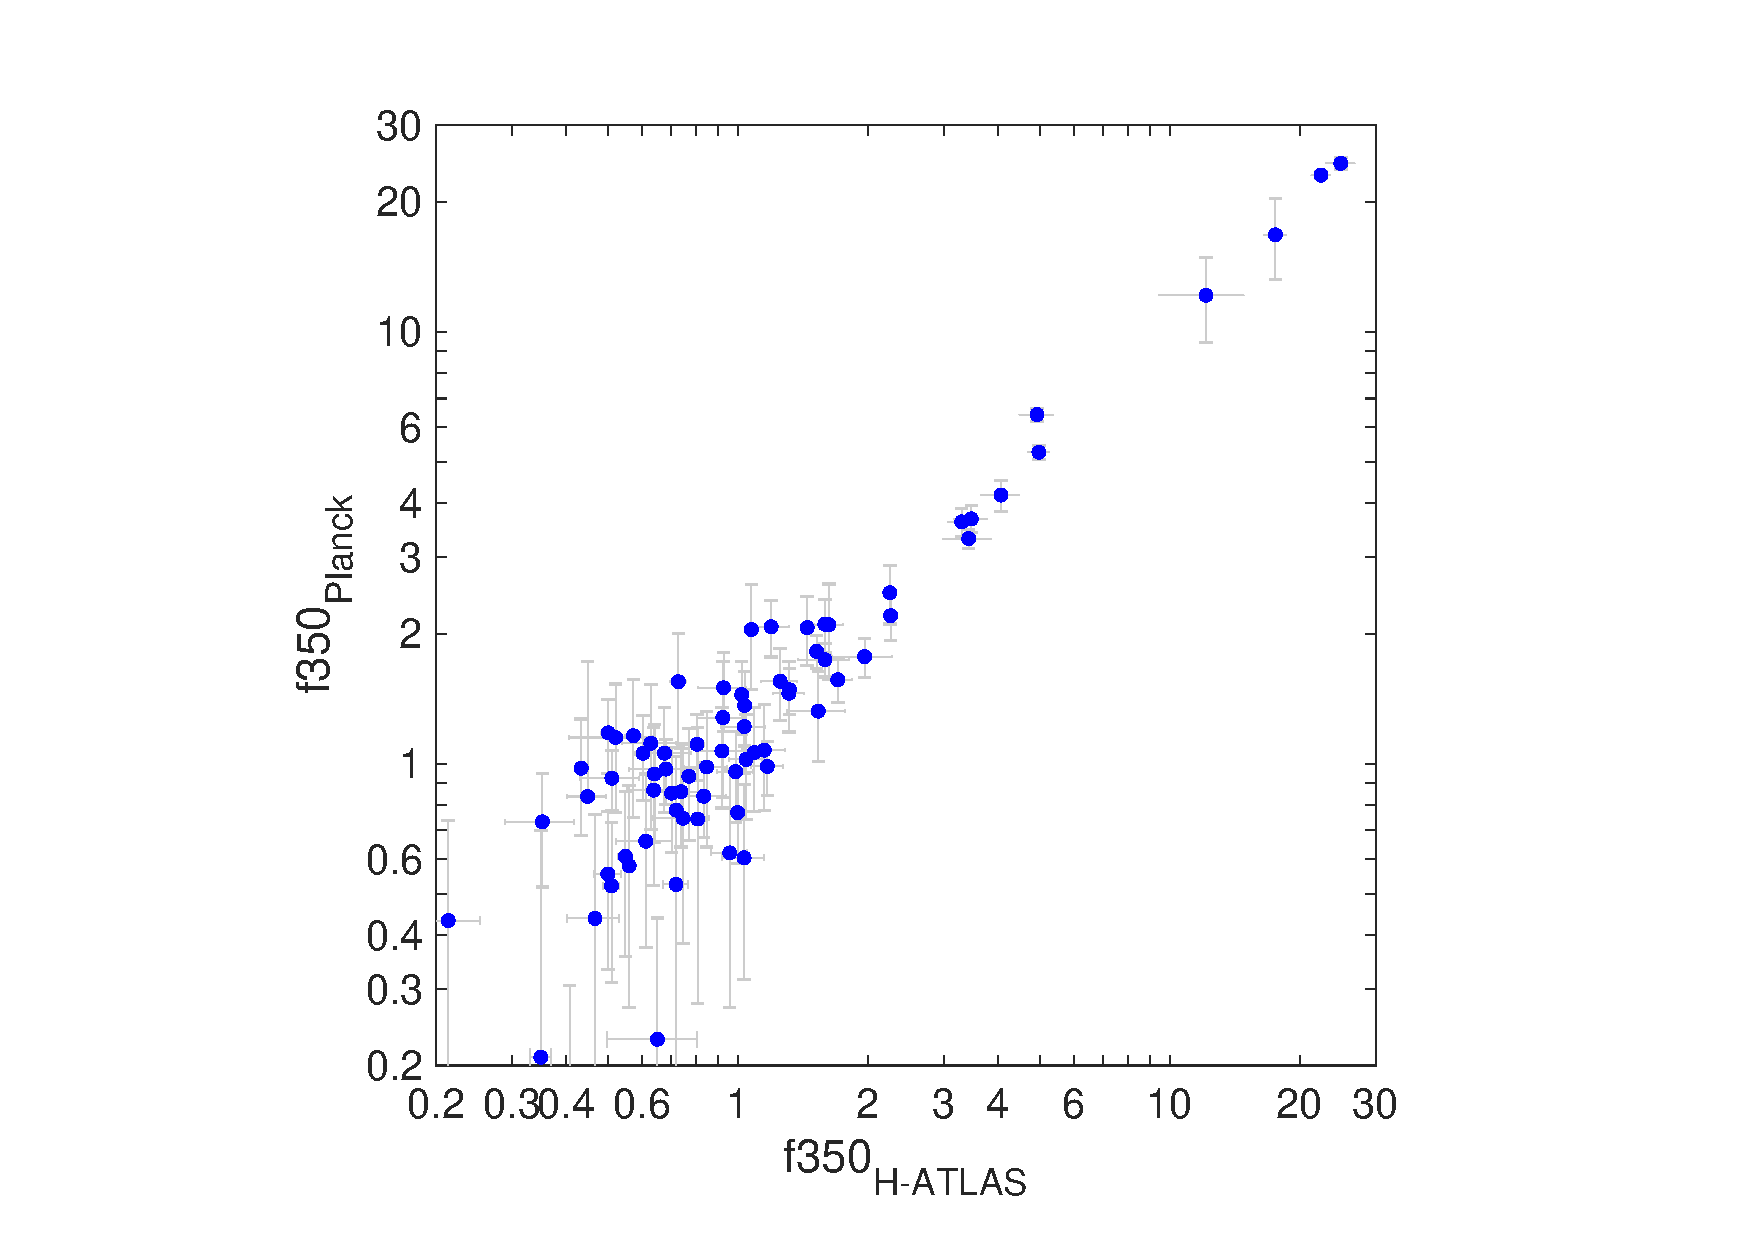
\includegraphics[width=0.6\textwidth, trim=40mm .0mm 0.0mm .0mm, clip=True]{planck_comp350}
  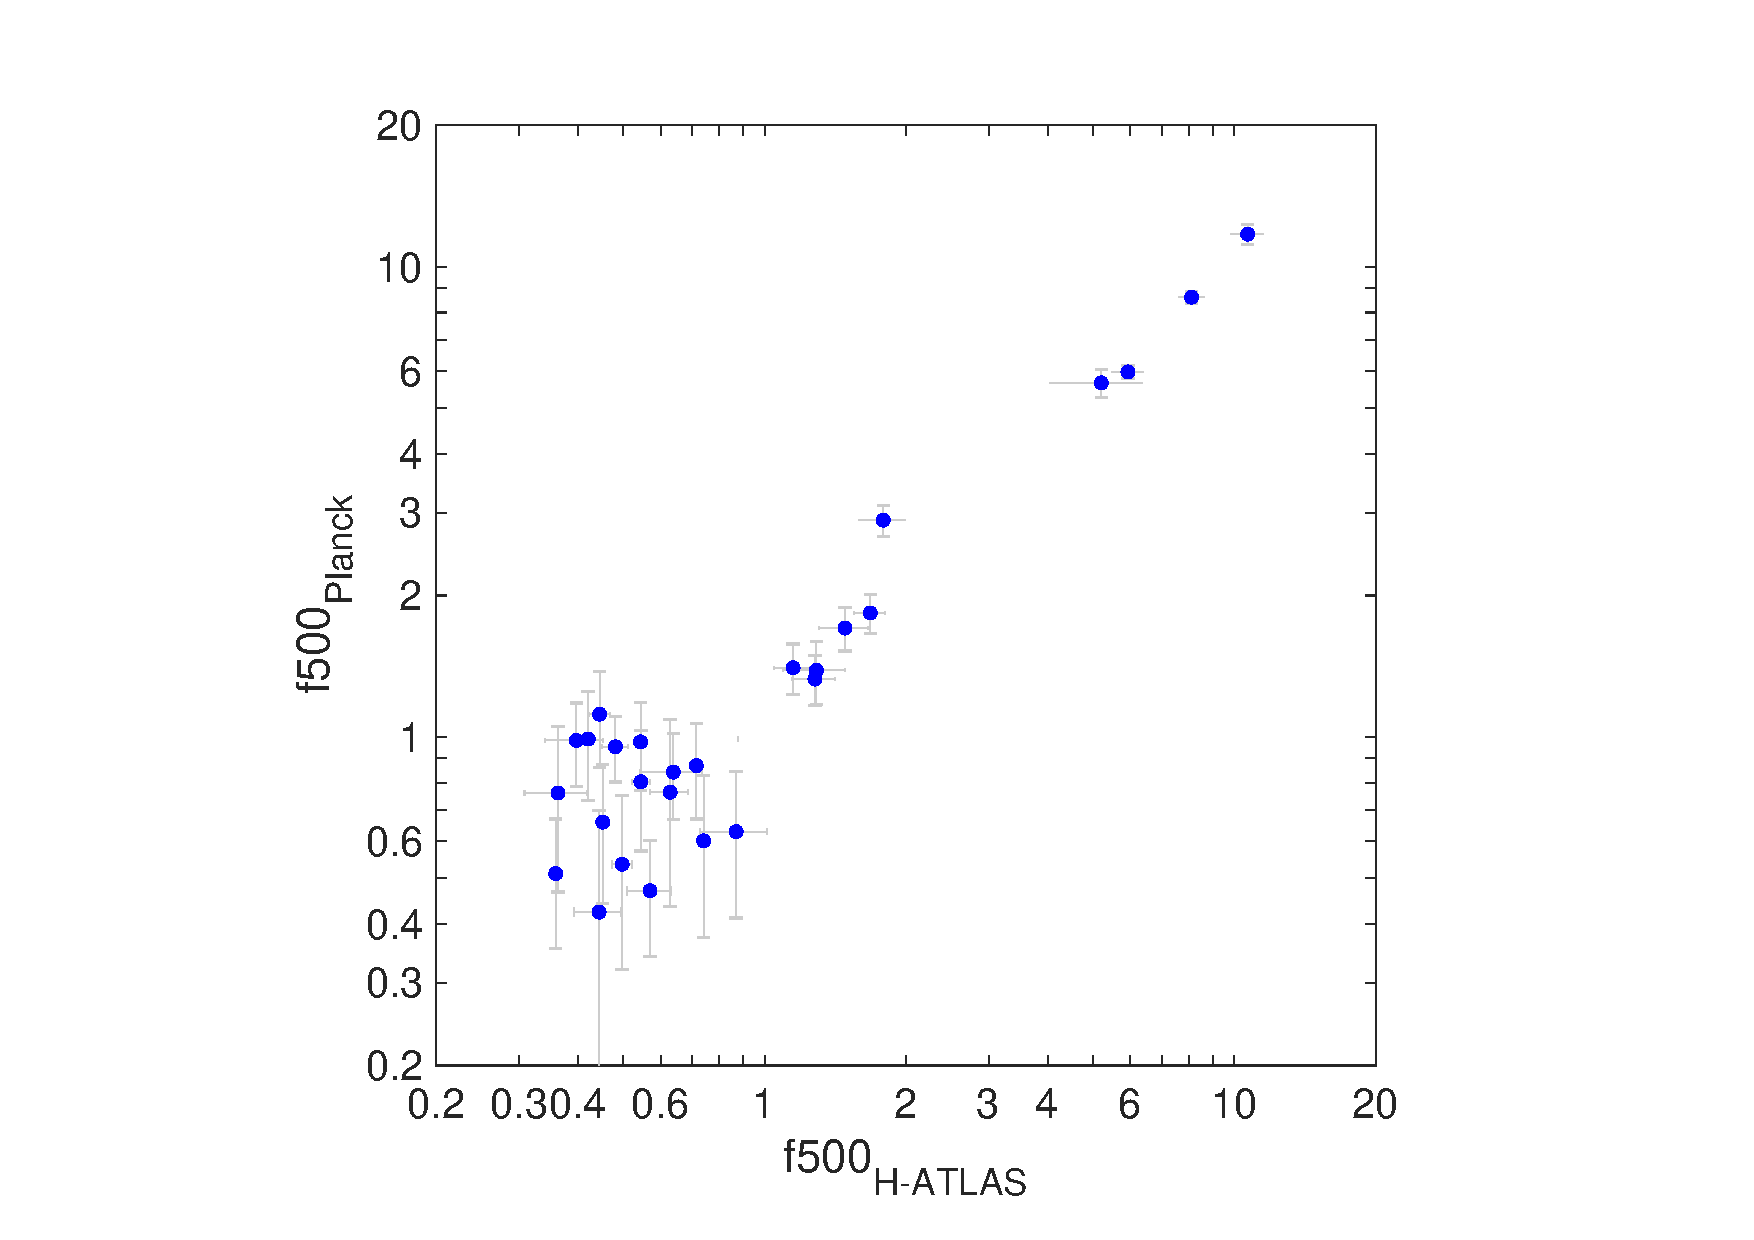
\includegraphics[width=0.6\textwidth, trim=40mm .0mm 0.0mm .0mm, clip=True]{planck_comp500}
  \caption{Comparison between H-ATLAS and Planck flux measurements for
    350\mic\ and 500\mic\ bands.}\label{fig:planck}
\end{figure}

% \begin{table*}[!h]
% \centering
% \caption{Comparison of HATLAS with \textit{Planck} flux densities (Jy,
%   rounded to 1\,mJy) at 350 and $500\,\mu$m for NGP sources.  }\label{tab:NGP}
% \begin{tabular}{ccccc}
%   \hline
%    HATLAS\_IAU\_ID          &     F350BEST       & F$_{\rm Planck350}$ &      F500BEST     & F$_{\rm Planck500}$ \\
%   \hline
%   HATLASJ125026.0+252947  & $12.128\pm 2.696$  & $12.128\pm 2.696$   & $5.208 \pm 1.160$ & $5.666\pm 0.393$ \\
%   HATLASJ132149.3+225342  & $5.820 \pm 3.611$  &     ---             & $0.058 \pm 0.151$ &       ---        \\
%   HATLASJ125440.7+285619  & $4.974 \pm 0.285$  & $5.254\pm  0.204$   & $1.678 \pm 0.126$ & $1.836\pm 0.176$ \\
%   HATLASJ131136.9+225454  & $3.469 \pm 0.304$  & $3.684\pm  0.265$   & $1.279 \pm 0.134$ & $1.328\pm 0.161$ \\
%   HATLASJ132035.3+340824  & $2.255 \pm 0.009$  & $2.199\pm  0.270$   & $0.715 \pm 0.009$ & $0.869\pm 0.200$ \\
%   HATLASJ133955.6+282402  & $1.701 \pm 0.131$  & $1.563\pm  0.181$   & $0.570 \pm 0.061$ & $0.471\pm 0.130$ \\
%   HATLASJ125144.9+254615  & $1.589 \pm 0.215$  & $1.740\pm  0.154$   & $0.639 \pm 0.096$ & $0.842\pm 0.176$ \\
%   HATLASJ131503.5+243709  & $1.588 \pm 0.008$  & $2.101\pm  0.298$   & $0.544 \pm 0.009$ & $0.976\pm 0.207$ \\
%   HATLASJ133457.2+340238  & $1.311 \pm 0.108$  & $1.454\pm  0.271$   & $0.444 \pm 0.051$ & $0.424\pm 0.275$ \\
%   HATLASJ125253.6+282216  & $1.168 \pm 0.099$  & $0.985\pm  0.142$   & $0.359 \pm 0.008$ & $0.512\pm 0.157$ \\
%   HATLASJ132815.2+320157  & $1.043 \pm 0.093$  & $1.022\pm  0.280$   & $0.362 \pm 0.044$ &       ---        \\
%   HATLASJ134308.8+302016  & $1.032 \pm 0.114$  & $0.605\pm  0.288$   & $0.319 \pm 0.009$ &       ---        \\
%   HATLASJ131206.6+240543  & $1.019 \pm 0.029$  & $1.444\pm  0.278$   & $0.385 \pm 0.020$ &       ---        \\
%   HATLASJ132255.7+265857  & $0.987 \pm 0.094$  & $0.958\pm  0.228$   & $0.330 \pm 0.045$ &       ---        \\
%   HATLASJ131612.2+305702  & $0.925 \pm 0.117$  & $1.498\pm  0.310$   & $0.346 \pm 0.055$ &       ---        \\
%   HATLASJ130547.6+274405  & $0.922 \pm 0.118$  & $1.278\pm  0.442$   & $0.363 \pm 0.055$ & $0.760\pm 0.292$ \\
%   HATLASJ130514.1+315959  & $0.832 \pm 0.104$  & $0.840\pm  0.165$   & $0.258 \pm 0.008$ &       ---        \\
%   HATLASJ130056.1+274727  & $0.769 \pm 0.023$  & $0.934\pm  0.269$   & $0.268 \pm 0.018$ &       ---        \\
%    HATLASJ131244.8+314832  & $0.754 \pm 0.097$  &  ---                & $0.295 \pm 0.046$ &       ---        \\
%   HATLASJ133026.1+313707  & $0.737 \pm 0.100$  & $0.861\pm  0.220$   & $0.267 \pm 0.047$ &       ---        \\
%   HATLASJ124610.1+304355  & $0.718 \pm 0.047$  & $0.525\pm  0.342$   & $0.241 \pm 0.009$ &       ---        \\
%   HATLASJ130125.2+291849  & $0.701 \pm 0.008$  & $0.854\pm  0.233$   & $0.232 \pm 0.009$ &       ---        \\
%    HATLASJ131909.4+283022  & $0.699 \pm 0.142$  &     ---             & $0.243 \pm 0.065$ &       ---        \\
%   HATLASJ130947.5+285424  & $0.680 \pm 0.122$  & $0.971\pm  0.168$   & $0.220 \pm 0.057$ &       ---        \\
%   HATLASJ130617.2+290346  & $0.675 \pm 0.103$  & $1.057\pm  0.288$   & $0.247 \pm 0.049$ &       ---        \\
%   HATLASJ131241.9+224950  & $0.650 \pm 0.154$  & $0.230\pm  0.209$   & $0.253 \pm 0.072$ &       ---        \\
%    HATLASJ134107.9+231656  & $0.636 \pm 0.068$  &    ---              & $0.189 \pm 0.009$ &       ---        \\
%   HATLASJ131101.7+293442  & $0.628 \pm 0.089$  & $1.114\pm  0.409$   & $0.189 \pm 0.008$ &       ---        \\
%   HATLASJ125108.4+284705  & $0.611 \pm 0.090$  & $0.661\pm  0.285$   & $0.245 \pm 0.043$ &       ---        \\
%    HATLASJ131432.5+304221  & $0.604 \pm 0.107$  &     ---             & $0.197 \pm 0.051$ &       ---        \\
%   HATLASJ133550.1+345957  & $0.602 \pm 0.025$  & $1.056\pm  0.236$   & $0.200 \pm 0.019$ &       ---        \\
%    HATLASJ130831.9+244159  & $0.582 \pm 0.026$  &     ---             & $0.216 \pm 0.019$ &       ---        \\
%    HATLASJ130850.5+320953  & $0.577 \pm 0.008$  &     ---             & $0.207 \pm 0.008$ &       ---        \\
%   HATLASJ132948.2+310748  & $0.559 \pm 0.017$  & $0.580\pm  0.308$   & $0.190 \pm 0.014$ &       ---        \\
%    HATLASJ133329.1+330235  & $0.552 \pm 0.080$  &     ---             & $0.173 \pm 0.038$ &       ---        \\
%   HATLASJ131730.6+310533  & $0.548 \pm 0.021$  & $0.610\pm  0.253$   & $0.196 \pm 0.016$ &       ---        \\
%    HATLASJ131700.0+340607  & $0.547 \pm 0.020$  &     ---             & $0.217 \pm 0.016$ &       ---        \\
%    HATLASJ133421.2+335619  & $0.537 \pm 0.009$  &     ---             & $0.181 \pm 0.009$ &       ---        \\
%   HATLASJ131327.0+274807  & $0.520 \pm 0.114$  & $1.149\pm  0.379$   & $0.195 \pm 0.053$ &       ---        \\
%   HATLASJ133554.6+353511  & $0.510 \pm 0.079$  & $0.925\pm  0.148$   & $0.187 \pm 0.038$ &       ---        \\
%   HATLASJ125008.7+330933  & $0.509 \pm 0.022$  & $0.521\pm  0.209$   & $0.190 \pm 0.017$ &       ---        \\
%   HATLASJ131745.2+273411  & $0.500 \pm 0.019$  & $1.178\pm  0.230$   & $0.169 \pm 0.015$ &       ---        \\
%    HATLASJ133824.5+330704  & $0.494 \pm 0.105$  &     ---             & $0.149 \pm 0.009$ &       ---        \\
%    HATLASJ131028.7+322044  & $0.363 \pm 0.008$  &     ---             & $0.452 \pm 0.008$ & $0.659\pm 0.216$ \\
% 	\hline
% \end{tabular}
% \end{table*}



\subsection{Colour corrections and flux calibration}

The large wavelength range within each of the SPIRE pass bands means
that both the size of the PSF and the power detected by SPIRE depend
on the spectral energy distribution of the source.  The SPIRE
data-reduction pipeline and ultimately our flux densities are based on
the assumption that the flux density of a source varies with frequency
as $\nu^{-1}$.  If the user knows the SED of a source, the flux
densities should be corrected using corrections from either table 5.7
or 5.8 from the SPIRE
handbook\footnote{\url{http://herschel.esac.esa.int/Docs/SPIRE/spire\_handbook.pdf}}
(Valtchanov 2017). It is important to apply these corrections, since
they can be quite large: for a point source with a typical dust
spectrum ($T=20$K, $\beta=2$) the multiplicative correction is 0.96,
0.94 and 0.90 at 250, 350 and 500 $\mu$m, respectively. The catalogue
fluxes have had no colour correction applied.

As with SPIRE, the PACS flux densities are also based on the
assumption that flux density of the source is proportional to
$\nu^{-1}$, and a correction is required for sources which follow a
different SED. The required corrections are described in the PACS
Colour-Correction
document\footnote{\url{http://herschel.esac.esa.int/twiki/pub/Public/PacsCalibrationWeb/cc\_report\_v1.pdf}}.

On top of all other errors, there is an additional error due to the
uncertain photometric calibration of {\it Herschel}. As in V16, we assume
conservative calibration errors of 5.5\% for the three SPIRE wavebands
and 7\% for PACS (see V16 for more details).

\section{The Catalogues}

We included all sources in the catalogues if they were detected above
4$\sigma$ in one or more of the three SPIRE bands: 250, 350 and
500 $\mu$m.  We eliminated all sources from the original list of point
sources produced by {\tt MADX} if they fell within the aperture of an
extended source. All of the H-ATLAS fields were observed at least
twice, making it possible to search for moving sources such as
asteroids. We found nine asteroids in the GAMA fields (V16), eliminating
these from the final catalogue. We carried out the same search for the
NGP and SGP but found no moving objects.


The sources in the final catalogues are almost all extragalactic
sources. We carried out a search for clusters of sources in all the
H-ATLAS fields (Eales et al. in preparation).  In the GAMA9 field, we
found several groups of sources that are likely to be clusters of
prestellar cores, implying that the catalogue for this field is likely
to contain a few tens of Galactic sources.  However, we found no
similar clusters in the other fields, which makes sense, since the
GAMA9 field is at a much lower Galactic latitude than the other
fields. Prestellar cores are therefore likely to be a very minor
contaminant to the catalogues for these fields. There are a few debris
disks and AGB stars in the catalogues, and an incomplete list is given
in Table 1.  However, well over 99\% of the sources are
extragalactic. The extragalactic sources range from galaxies at
redshift 6 (Fudamoto et al. 2017) to nearby galaxies, such as the
spectacular spiral galaxy, NGC 7793, which is in the centre of the
SGP, and one of the brightest galaxies in the nearby Sculptor group.

\subsection{Statistics of the catalogues}

The catalogue for the NGP contains 118,986 sources, of which 112,074
were detected at $>4\sigma$ at 250 $\mu$m, 46,872 at $>4\sigma$ at 350
$\mu$m and 10,369 at $>4\sigma$ at 500 $\mu$m. The effective
sensitivity of the PACS images was much less, but the catalogues
contain flux-density measurements at 100 $\mu$m and 160 $\mu$m for all
the sources in the catalogue. 4,207 sources were detected at
$>3\sigma$ at 100 $\mu$m and 6,342 sources were detected at $>3\sigma$
at 160 $\mu$m.


\begin{deluxetable}{cl}
\tablecaption{Stars in H-ATLAS}
\tablecolumns{2}
\tablewidth{0pt}
\tablehead{ \colhead{Name} & \colhead{Position}}
\startdata
EY Hya & 08:46:21.4 $+$01:37:53 \\
IN Hya & 09:20:36.7 $+$00:10:53 \\
NU Com & 13:10:08.5 $+$24:36:02 \\
19 PsA & 22:42:22.3 $-$29:21:43 \\
V PsA & 22:55:19.9  $-$29:36:48 \\
S Sci & 00:15:22.4 $-$32:02:44 \\
XY Sci & 00:06:35.9 $-$32:35:38 \\
eta Sci & 00:27:55.9 $-$33:00:27 \\
Y Sci & 23:09:05.7 $-$30:08:04 \\
HD 119617 & 13:43:35.2 $+$35:20:45 \\
R Sci & 01:26:58.2 $-$32:32:37 \\
Fomalhaut & 22:57:39.2 $-$29:37:22 \\
\enddata
\end{deluxetable}

The catalogue for the SGP contains 193,536 sources, of which 182,210 were
detected at $>4\sigma$ at 250 $\mu$m, 74,061 at $>4\sigma$ at 350 $\mu$m
and 16,076 at $>4\sigma$ at 500 $\mu$m.  5500 sources were detected at
$>3\sigma$ at 100 $\mu$m and 10,86 sources were detected at $>3\sigma$
at 160 $\mu$m.

The cumulative number of sources as a function of signal-to-noise in
the five bands is shown in Figure~\ref{fig_sn}. The 250-\micron\ band is
the most sensitive, and so has the largest number of detected sources. Of
the PACS bands, the 160-\micron\ band detects most sources above
3-$\sigma$.

\begin{figure}
  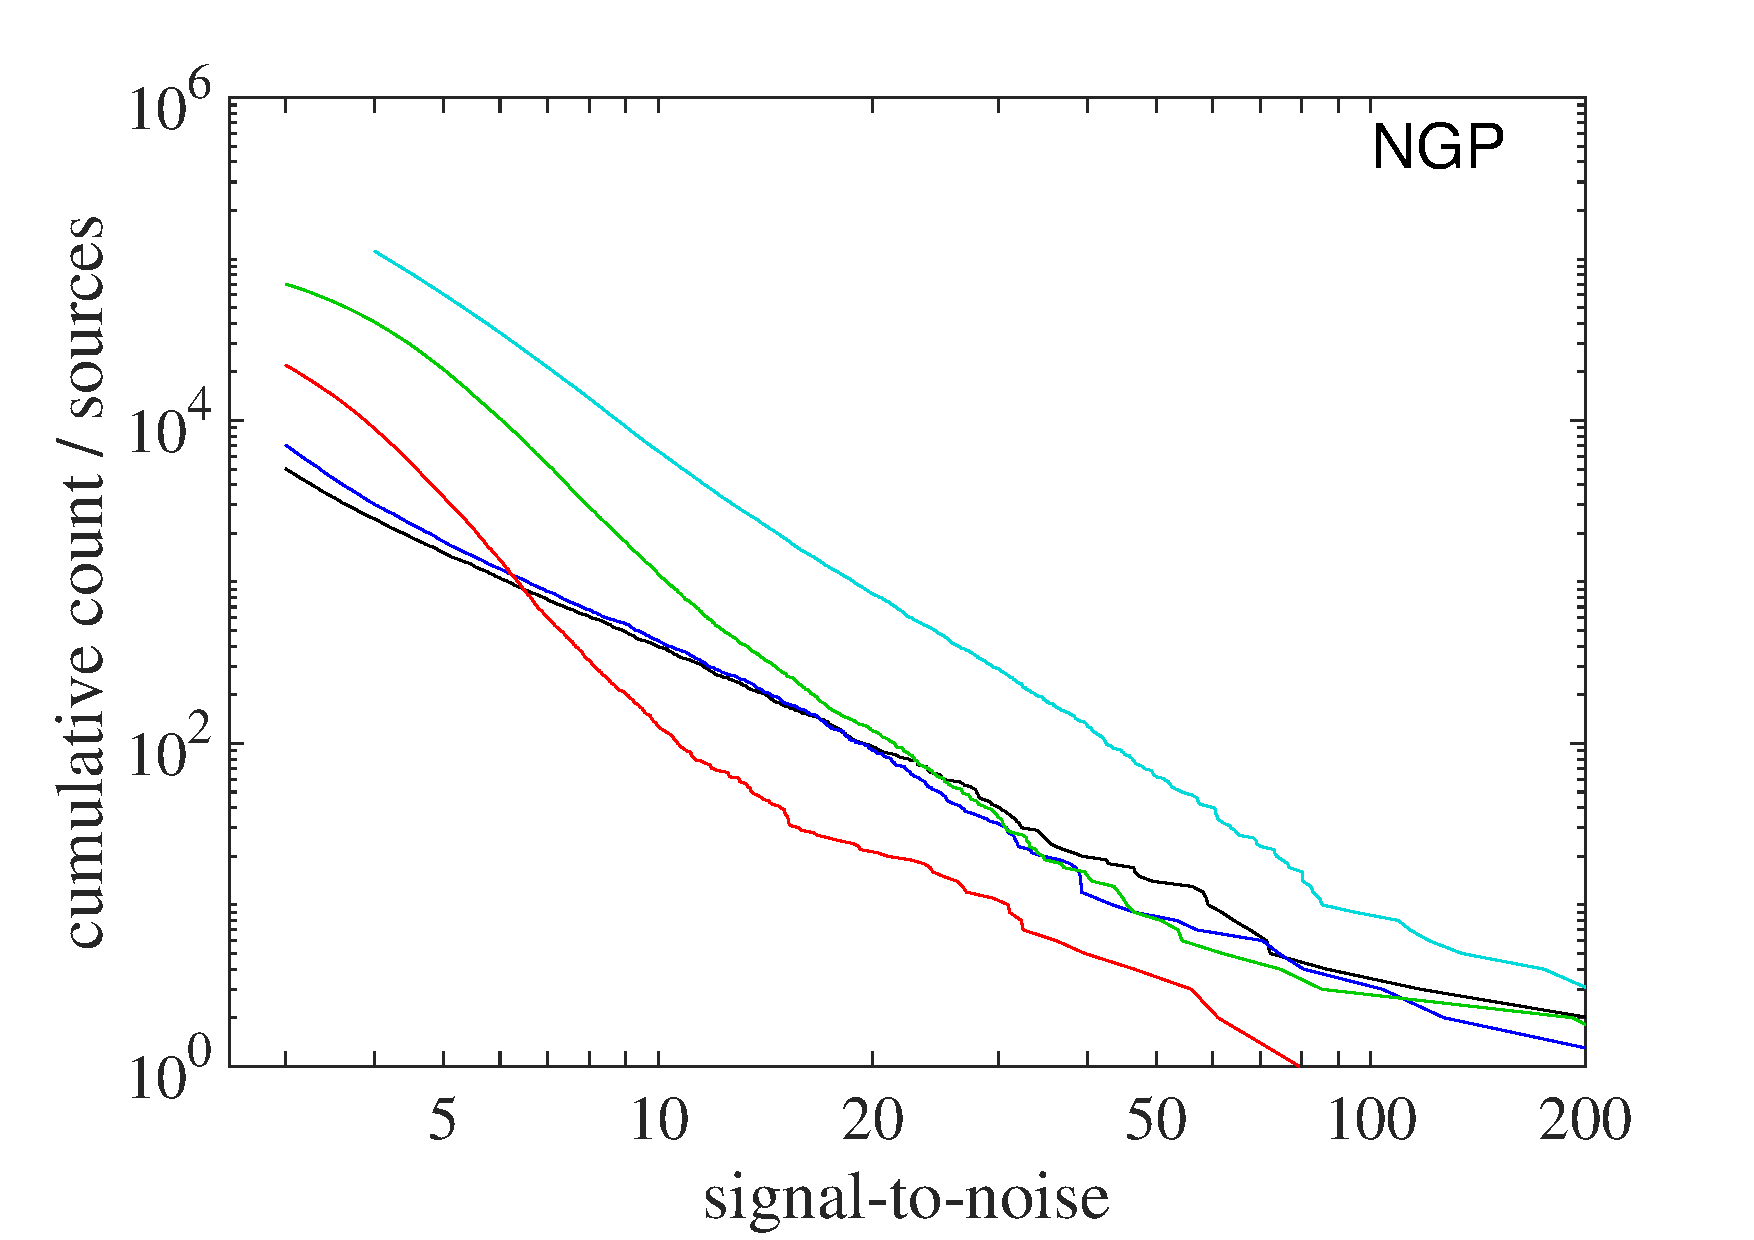
\includegraphics[width=0.5\textwidth]{cum_sn_best_NGP.pdf}
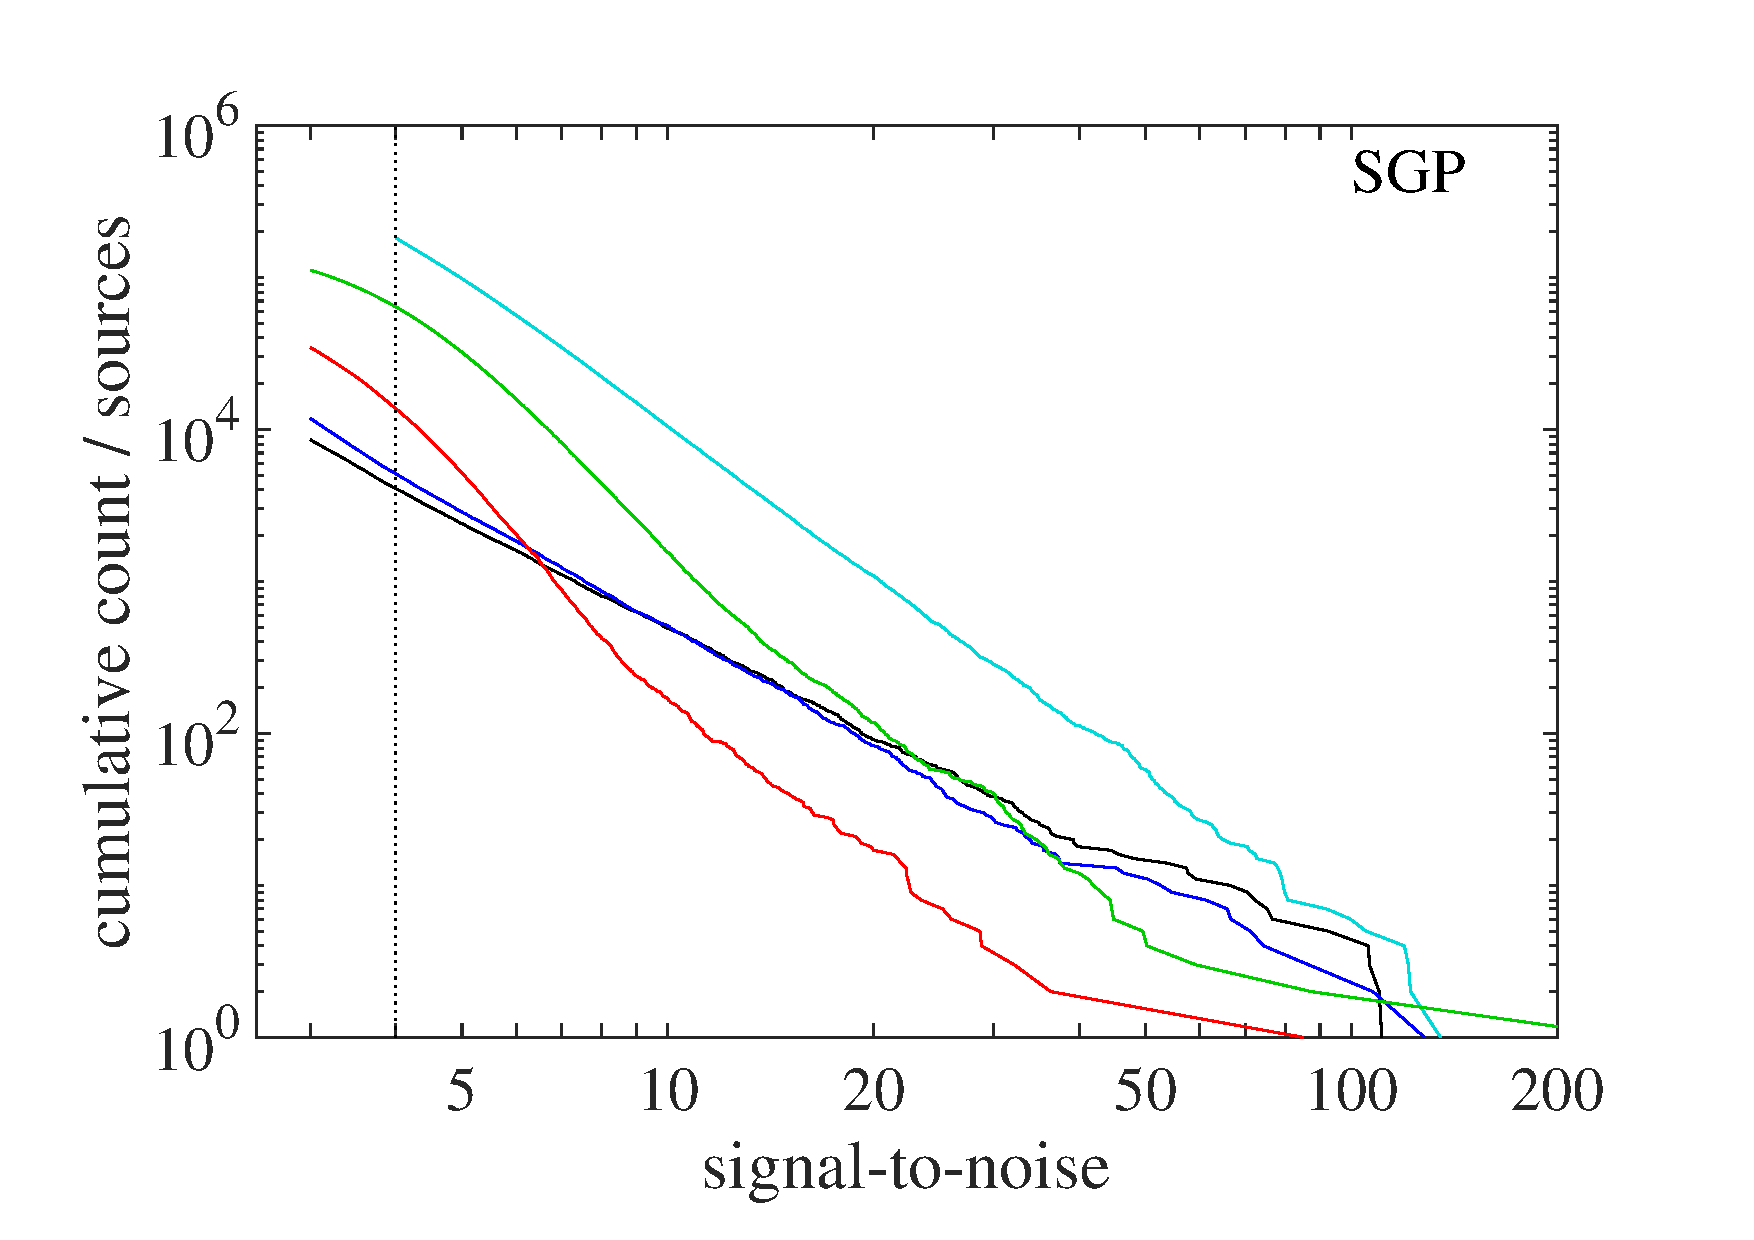
\includegraphics[width=0.5\textwidth]{cum_sn_best_SGP.pdf}
 \caption{\protect\label{fig_sn} The cumulative number of sources as a function
   of signal-to-noise at 100\mic\ (black), 160\mic\ (blue), 250\mic\ (cyan),
  350\mic\ (green) and 500\mic\ (red). The NGP area is shown in the top panel,
  and the SGP in bottom panel. The vertical dotted line shows the
  4-$\sigma$ limit for the 250\mic\ selection. The other bands are
  truncated at 3-$\sigma$.  
} 
\end{figure}


The observed number of sources as function of flux density in the PACS and
SPIRE bands is shown in Figure~\ref{fig_cum_flux}.  Note that this is
the observed flux in the catalogue, before any corrections are made
for source SED (Section 3.3) or ``flux boosting'' (Section 4.3), which
are necessary before the flux densities are compared with model
predictions. 

\begin{figure}
\textsl{}  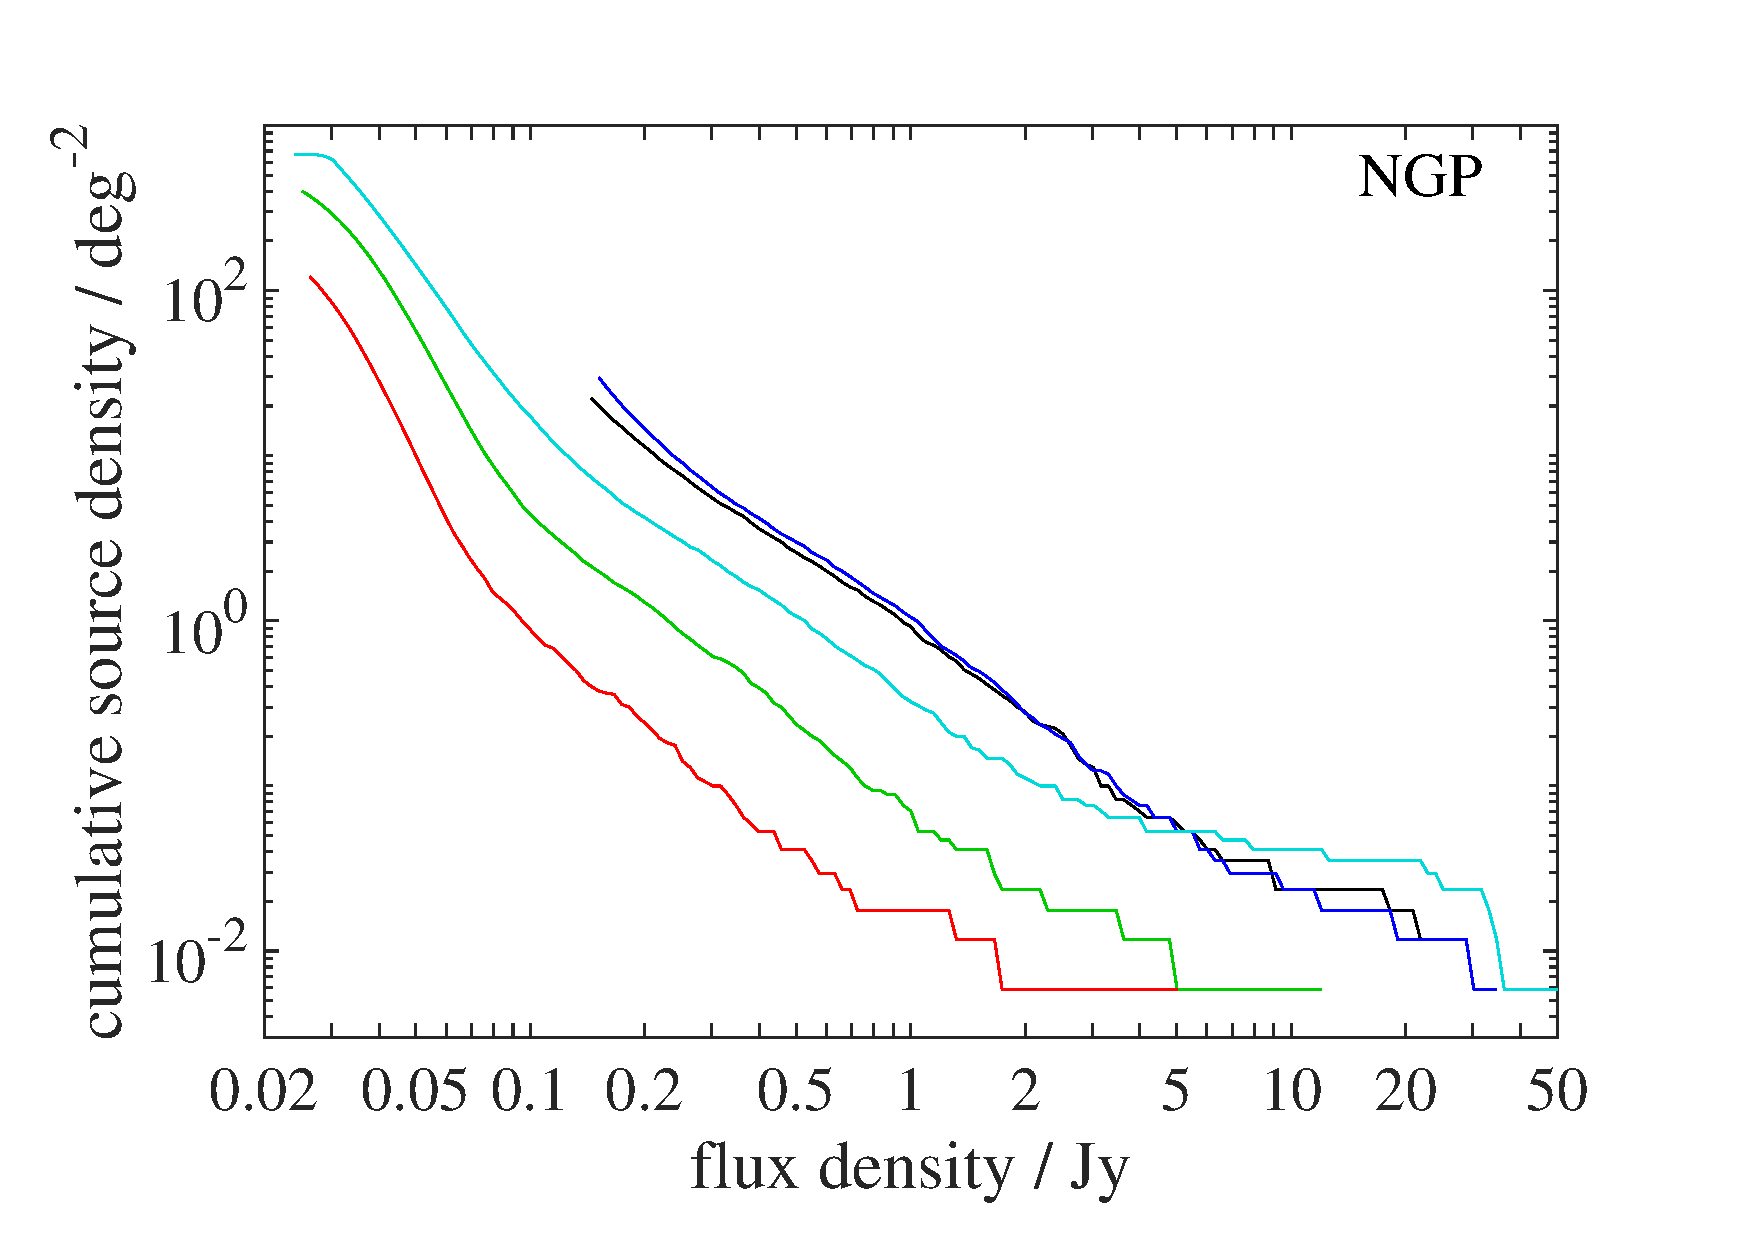
\includegraphics[width=0.5\textwidth]{cum_counts_best_NGP.pdf}\\
  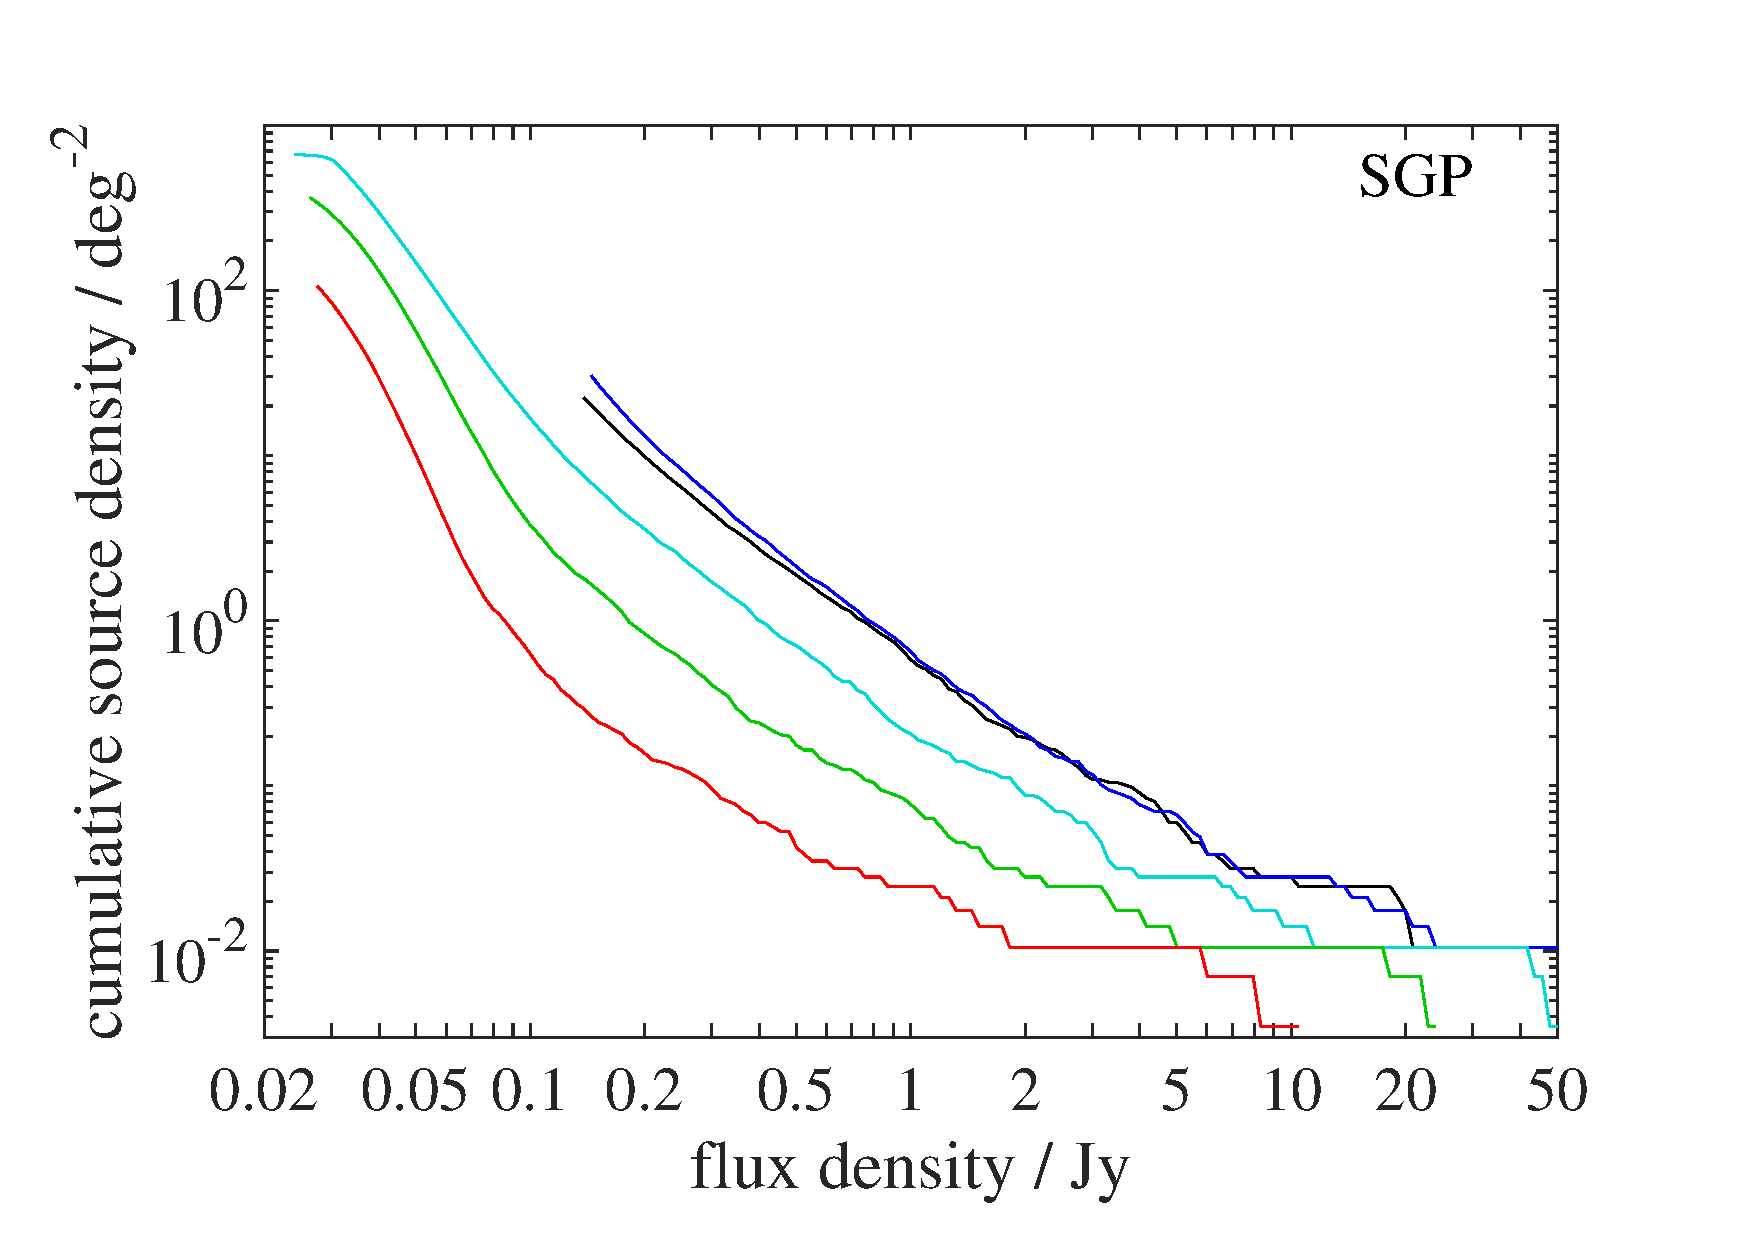
\includegraphics[width=0.5\textwidth]{cum_counts_best_SGP.pdf}
  \caption{\protect\label{fig_cum_flux} The cumulative number of
    sources as a function of flux at 100\mic\ (black), 160\mic\ (blue),
    250\mic (cyan), 350\mic\ (green) and 500\mic\ (red). The NGP area is
    shown in the top panel, and the SGP in the bottom panel. The
    counts are plotted only above the limit of 3$\sigma$ in each wave
    band.  }
\end{figure}  

\subsection{Positional Accuracy}

V16 carried out extensive simulations to investigate the accuracy of
the H-ATLAS catalogues by injecting artificial sources on to the GAMA
images, and then using {\tt MADX} to detect the sources and measure their
flux densities and positions. The results of these ``in-out''
simulations apply to the NGP and SGP catalogues, which were produced
using almost exactly the same methods.

We investigated the accuracy of the source positions in two ways: (1)
by looking at the positional offsets between the {\it Herschel}
sources and galaxies found on optical images; (2) from the in-out
simulations.  Bourne et al. (2016) and F17 describe the details of the
first method, which takes account of the clustering of the galaxies in
the optical catalogue and the PSF of the {\it Herschel} observations.
% We also use the positions of the galaxies to correct the astrometry of
% the individual {\it Herschel} observations, which ties the positions
% of the {\it Herschel} sources to the astrometric frame of the optical
% catalogue (S17).
Note that astrometric offsets were first calculated using catalogues
from individual {\it Herschel} observations. The astrometry for each
observation was updated before creating the final maps (S17).

In the case of the NGP, we applied this method using the galaxies
found in the SDSS $r$-band images (F17), which thus ultimately ties the
{\it Herschel} positions to the SDSS astrometric frame.   In the case
of the SGP, we used the galaxies found in the VLT Survey Telescope
ATLAS (Shanks et al.  2015), which thus ultimately ties the
astronometry in the SGP to the astrometric frame of this survey.  We
find that the positional error, $\sigma_\mathrm{pos}$, varies from
1.2 to 2.4 arc seconds as the signal-to-noise in flux varies from 10 to 5,
with a relationship between positional accuracy and flux density given
by $\sigma_\mathrm{pos} = 2.4 (\mathrm{SNR}/5)^{-0.84}$.  This agrees
well with the errors in the measured positions of the artificial
sources in the in-out simulations (V16).

%\begin{figure}
%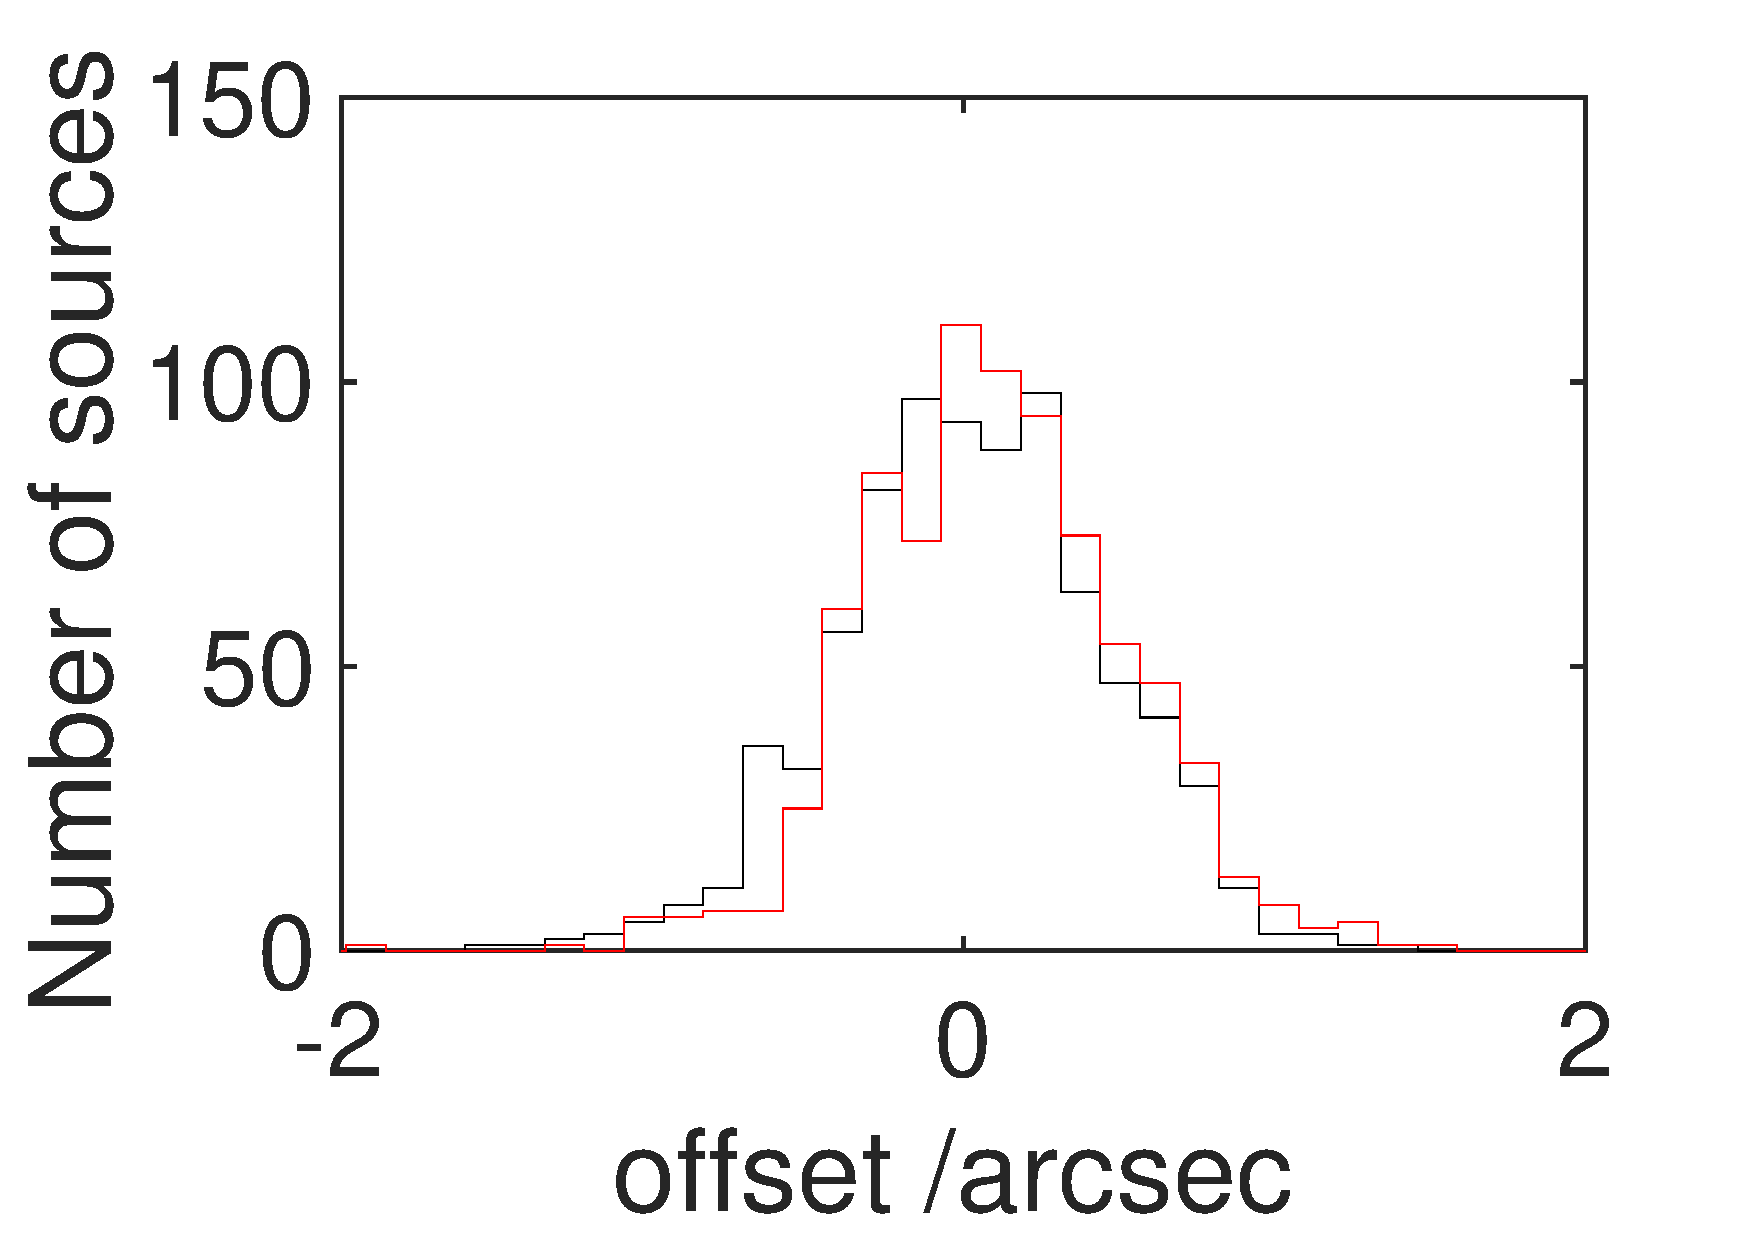
\includegraphics[scale=0.3]{ngp_pos_err_hist.pdf}
%\caption{\protect\label{fig_pos_err_hist} The distribution of
%  positional offsets between SPIRE and SDSS sources in the NGP. 
%The black histogram shows the offsets in RA, and the red line the
%offsets in DEC. 
%!!!IS this the map alignment histogram or the XID one? Which sources are included?
%}
%\end{figure}

The mean positional errors as a function of position within the NGP
and SGP fields are shown in Fig.~\ref{fig_pos_errs}. Though there are
hints of systematic variations in different parts of the fields, these
are around 1 arcsec, less than the quoted absolute pointing accuracy of
{\it Herschel} of $\simeq$2 arcsec (Pilbratt et al. 2010).

\begin{figure*}
%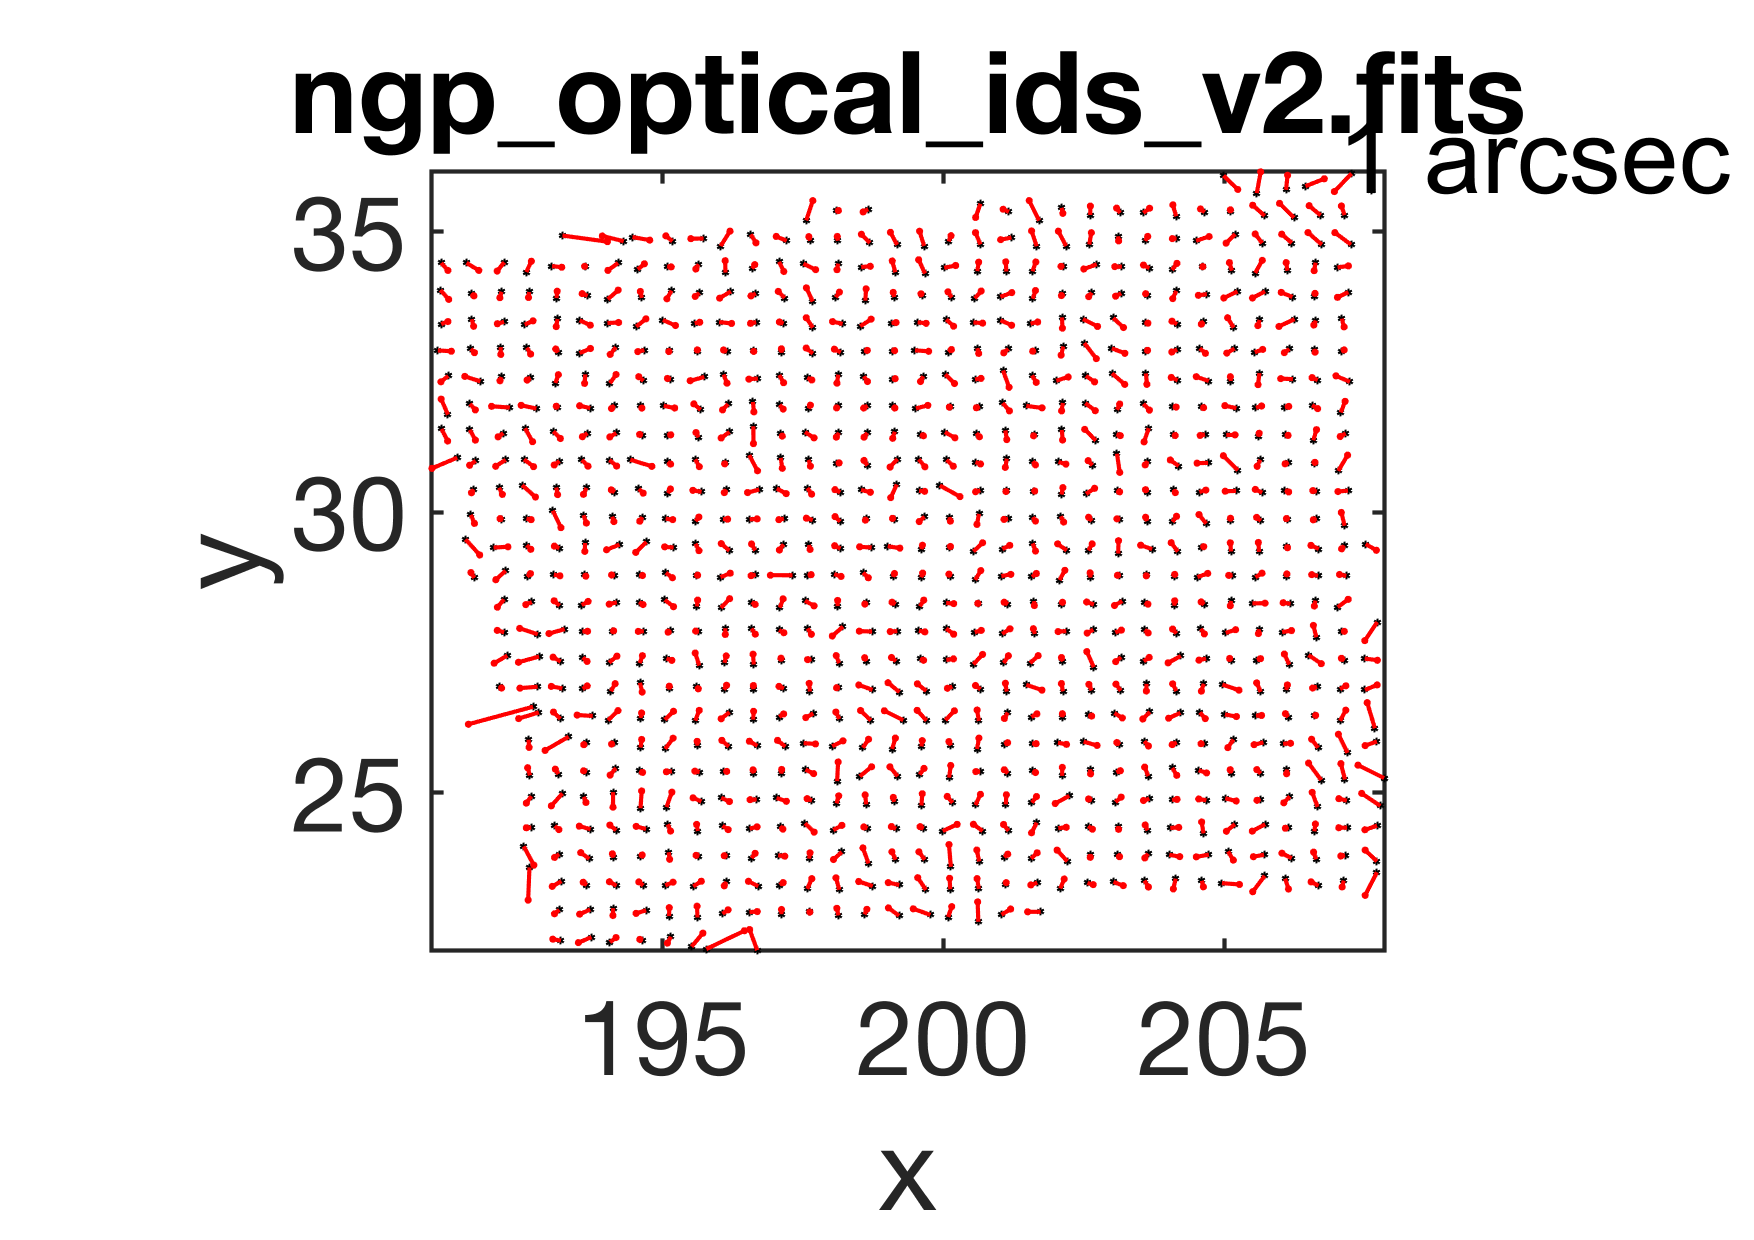
\includegraphics[scale=0.3]{ngp_posn_errors_new.pdf}
%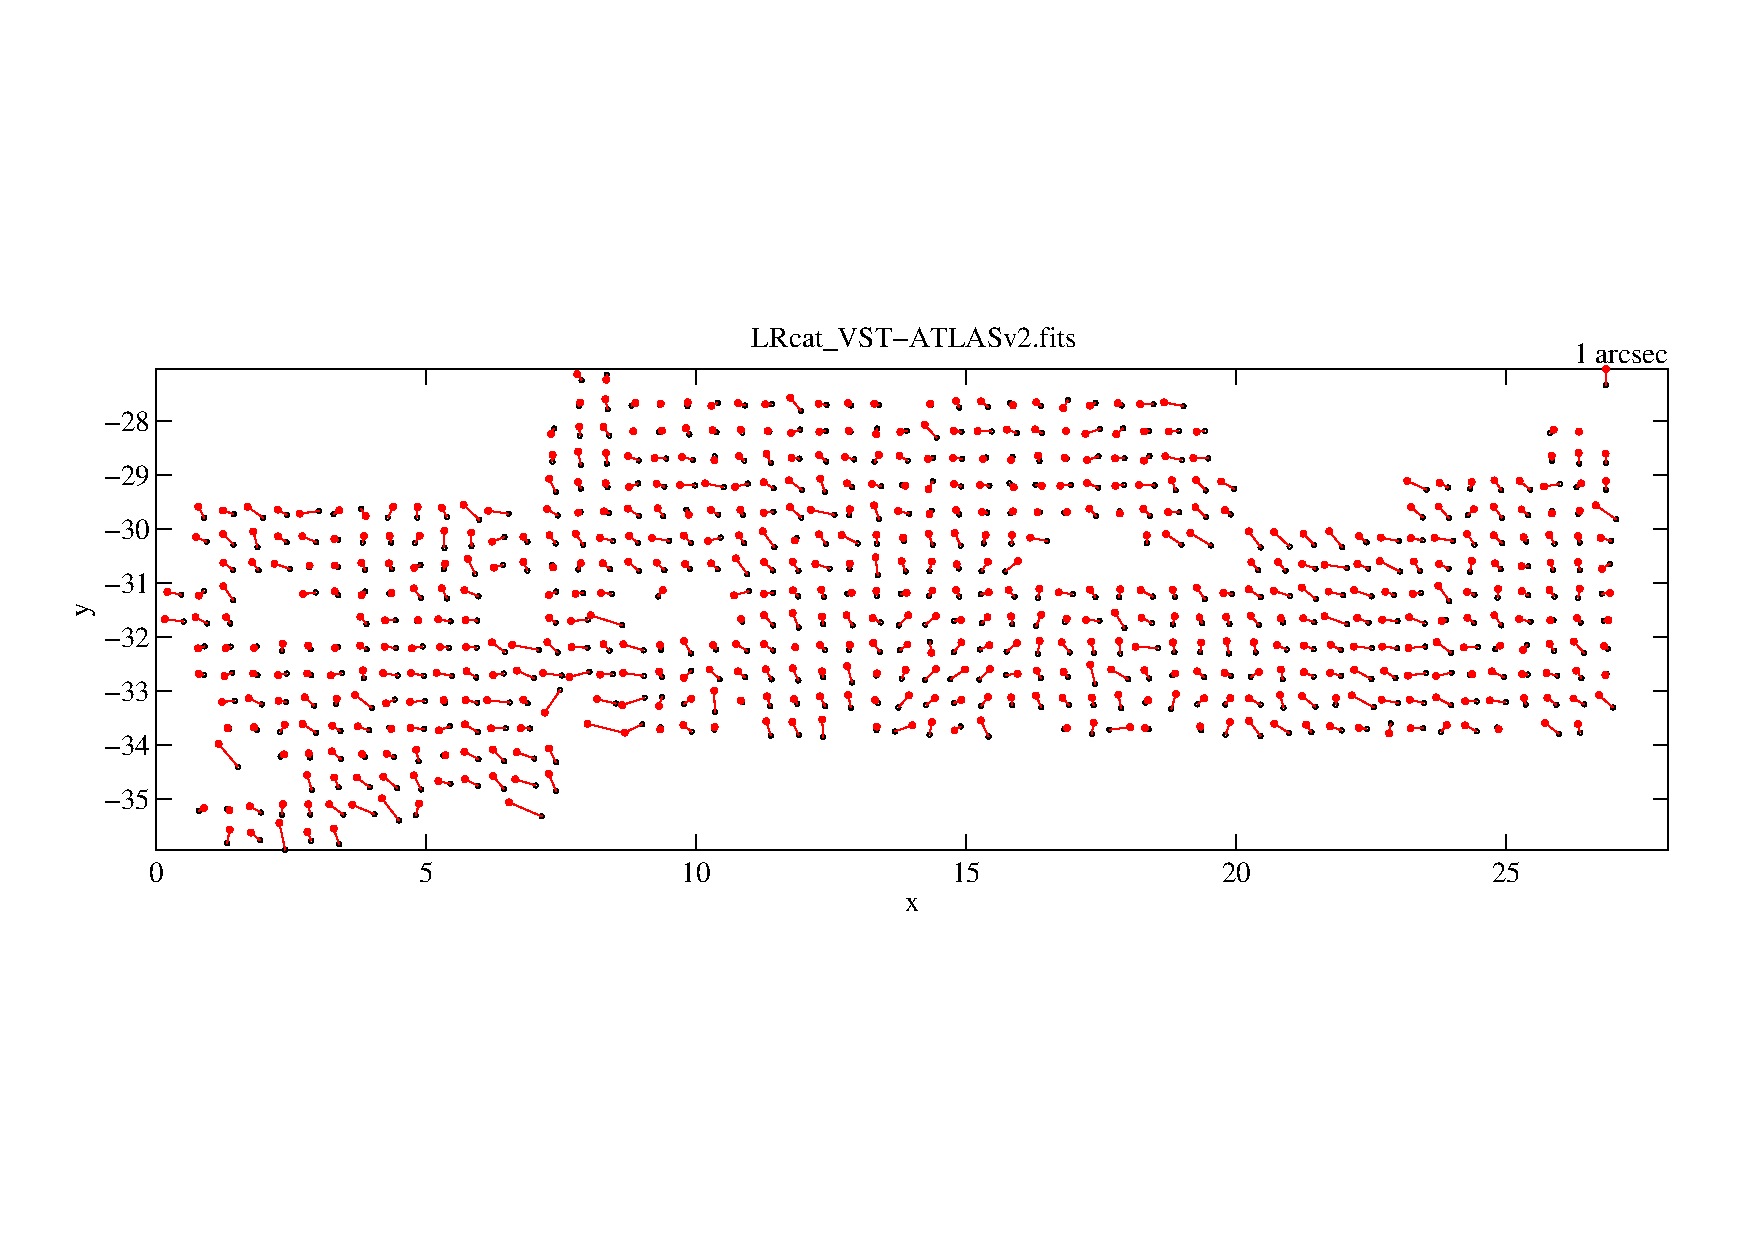
\includegraphics[scale=0.3,trim=0 45mm 0mm 45mm]{sgp_astrometry2.pdf}
%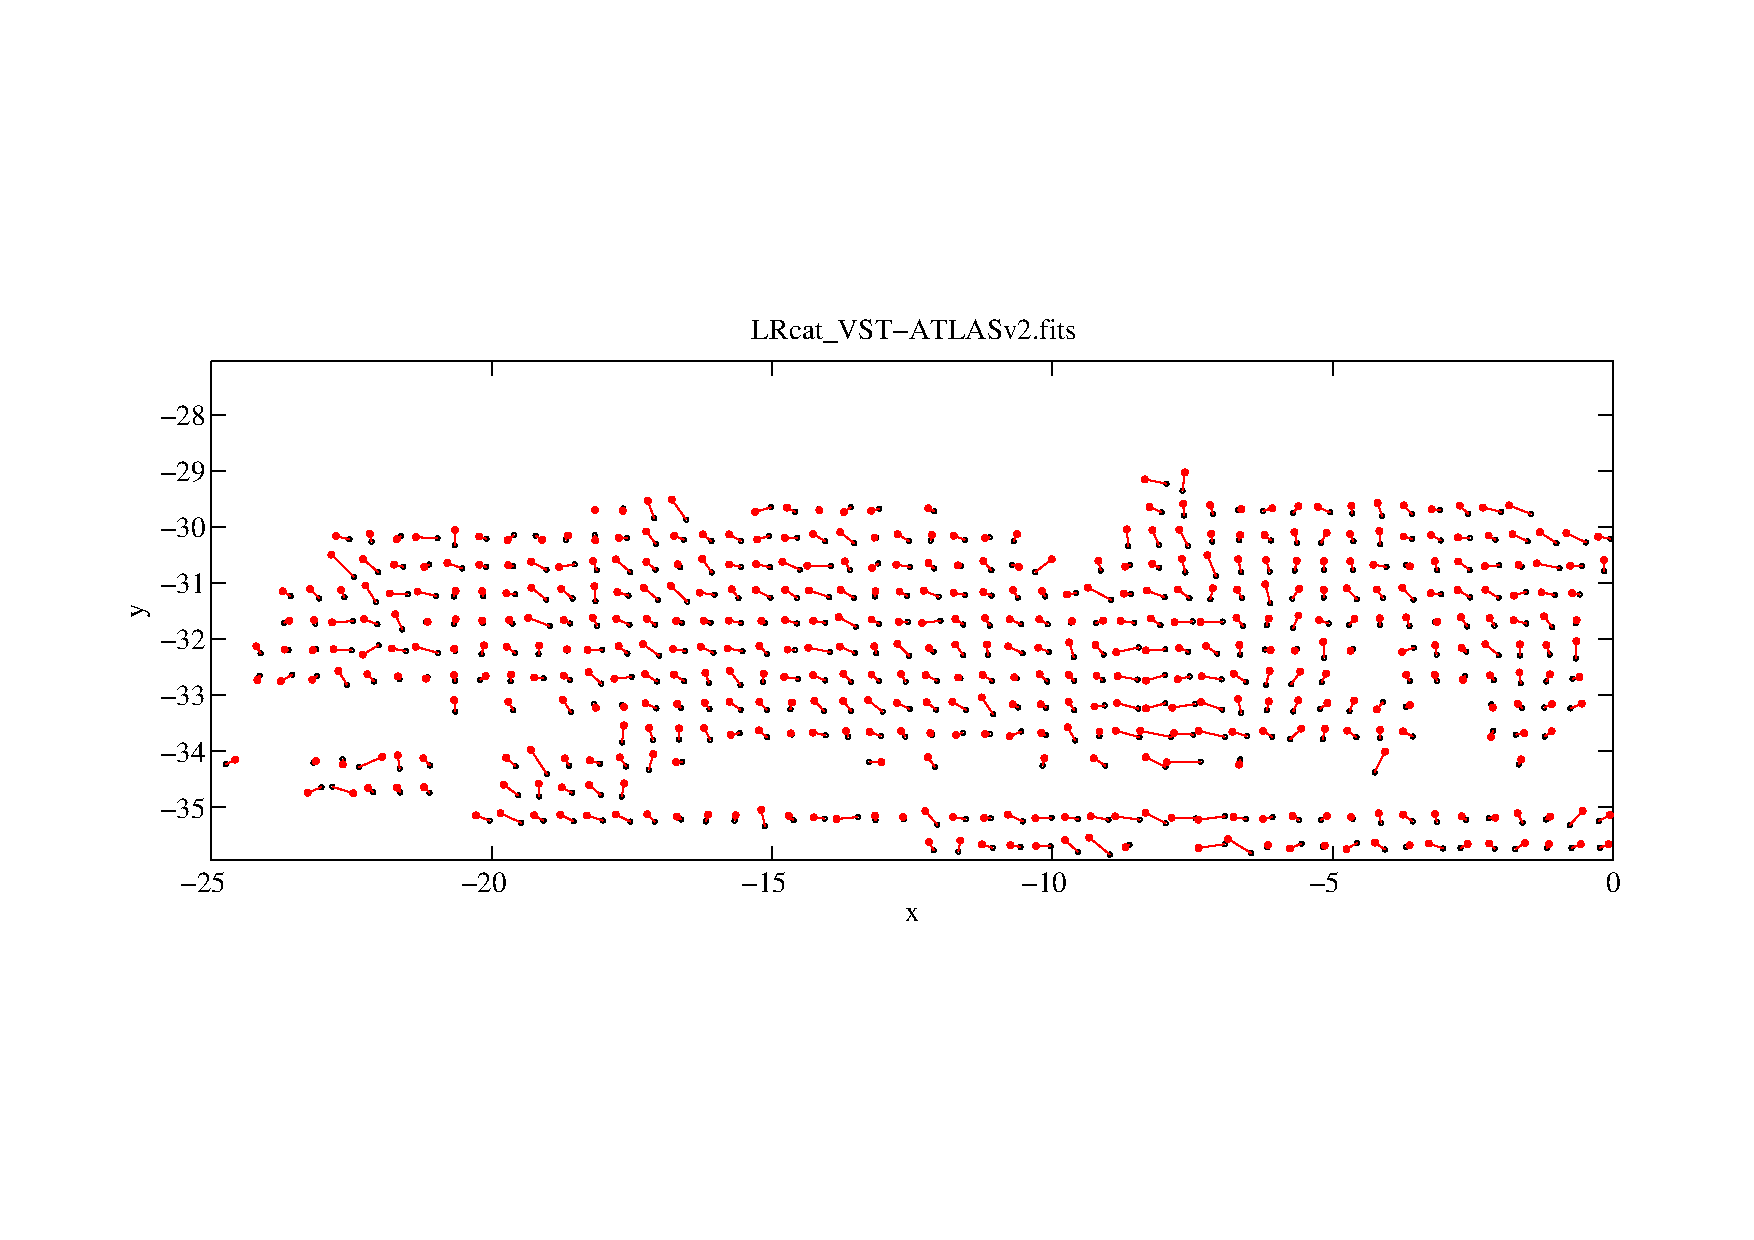
\includegraphics[scale=0.3,trim=0 45mm 0mm 45mm]{sgp_astrometry1.pdf}
\hspace{10mm}
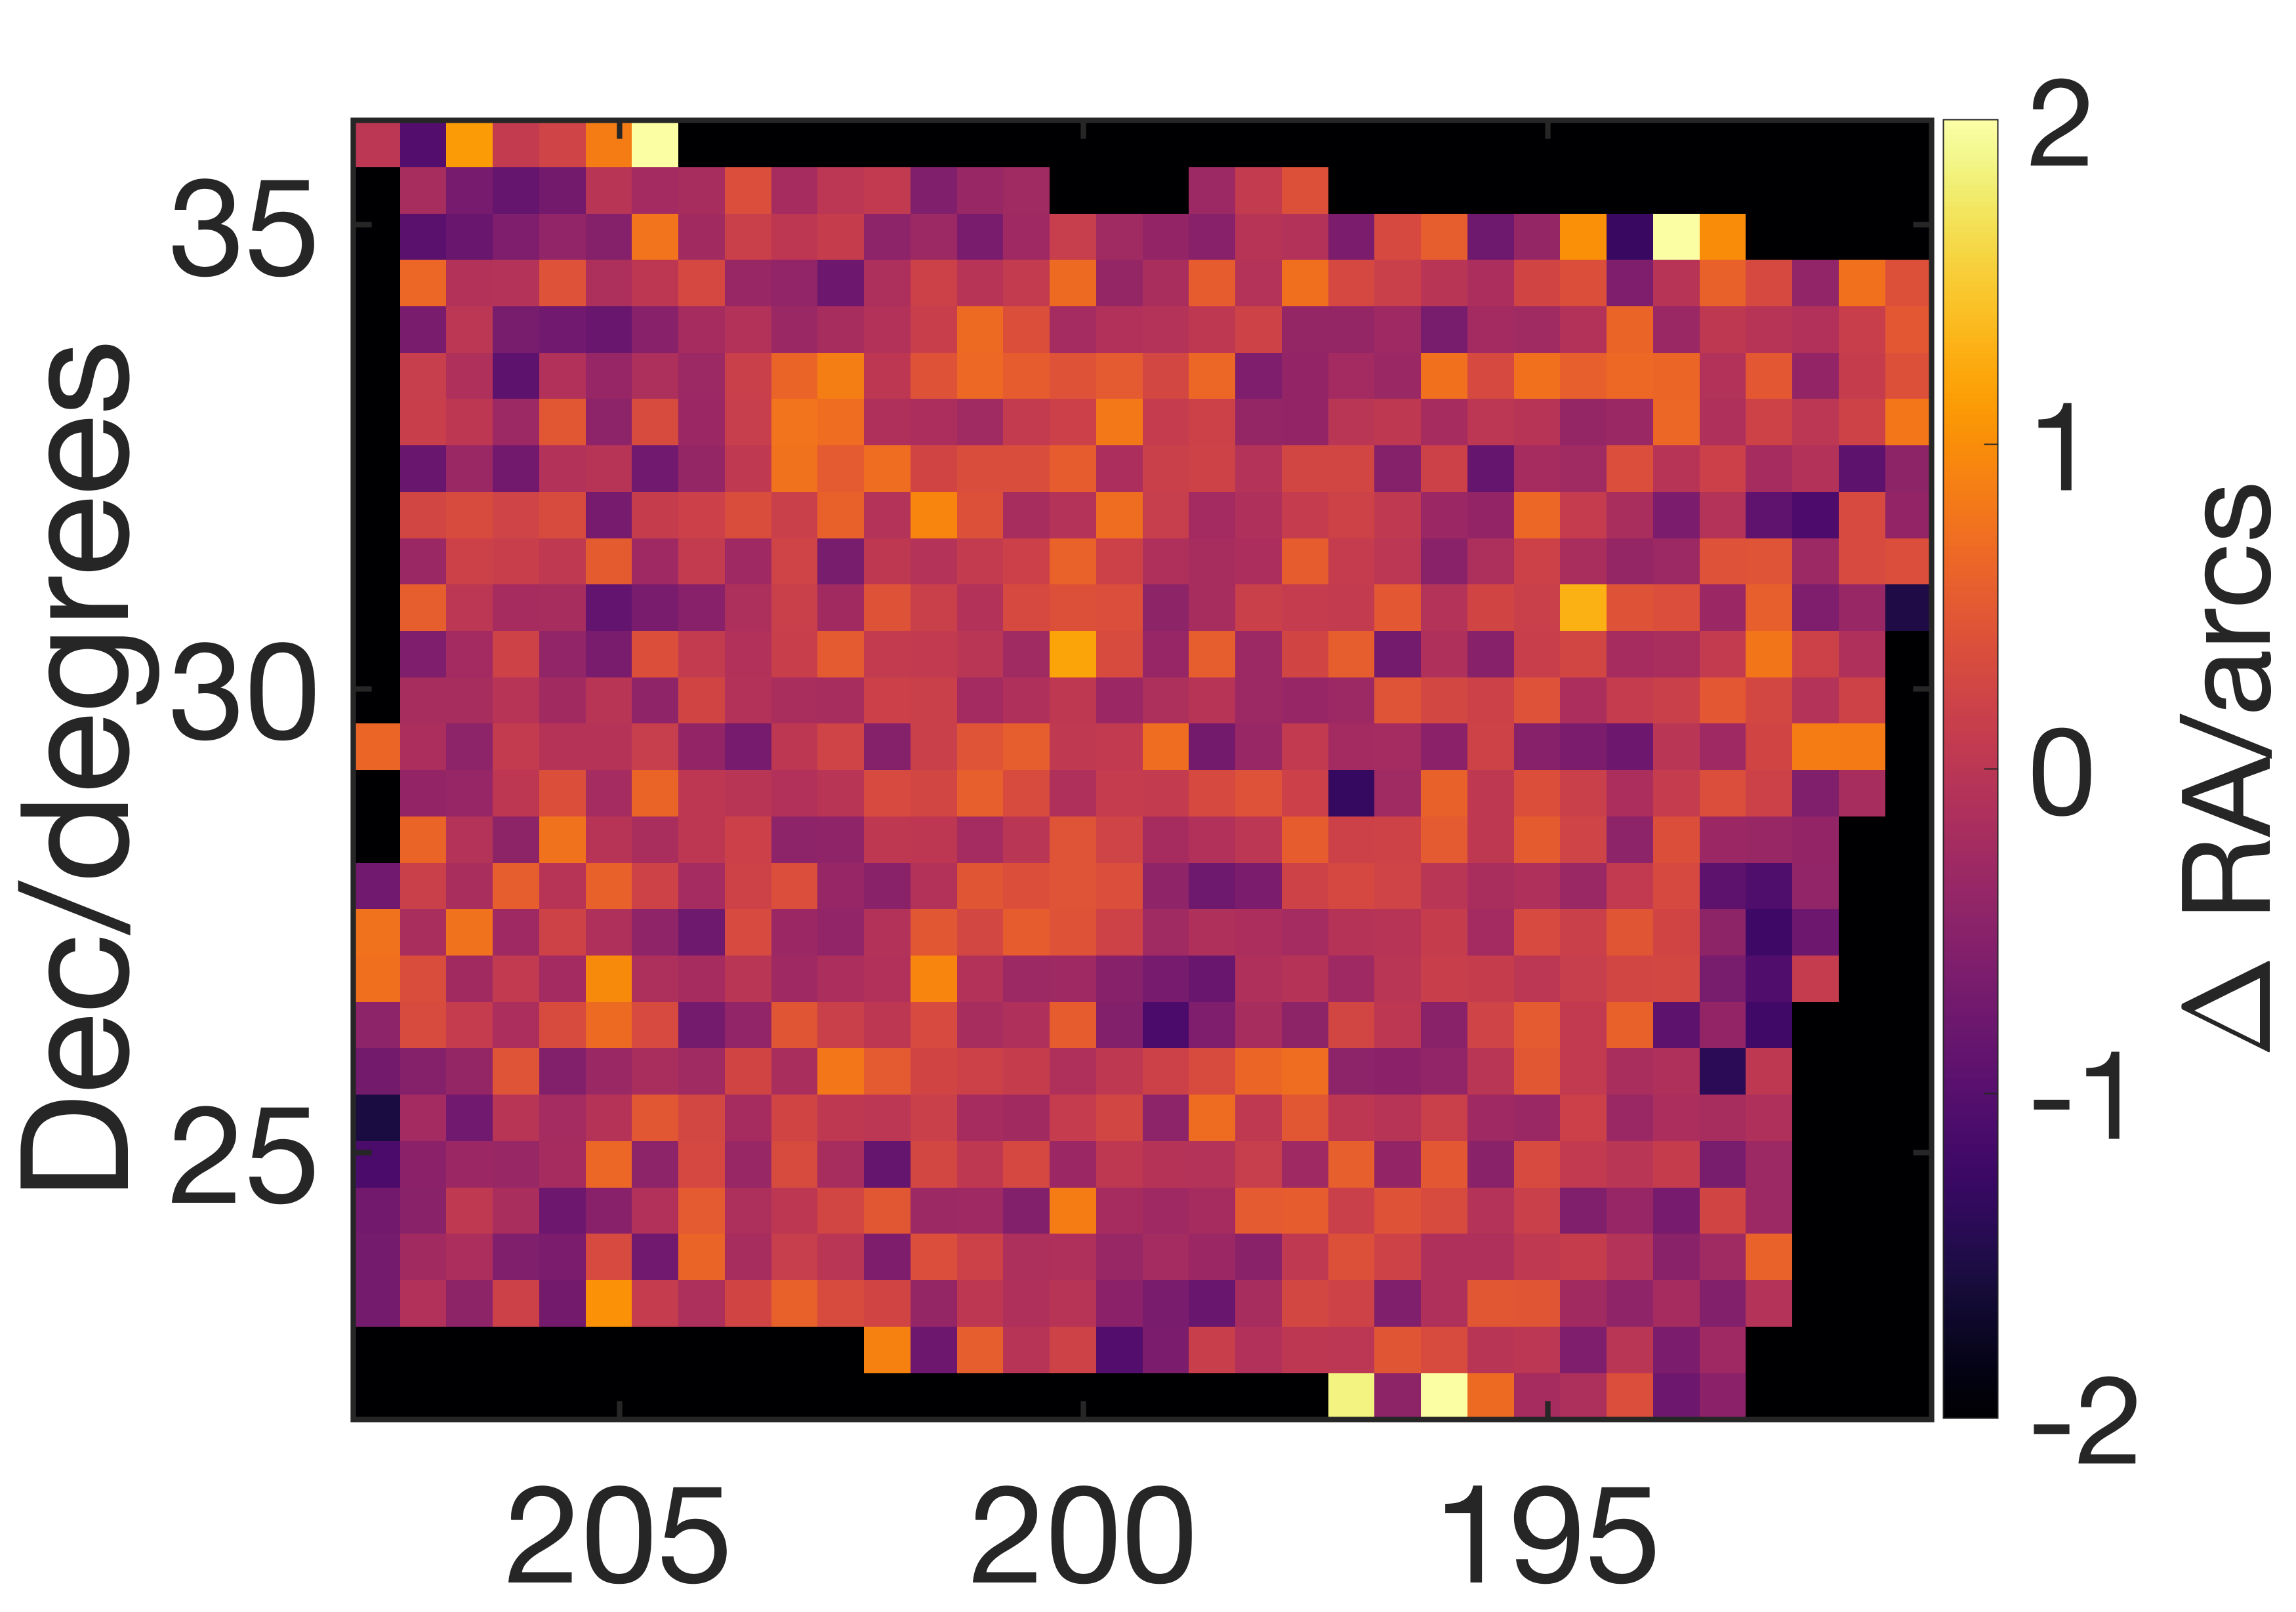
\includegraphics[scale=0.23]{ngp_dra.png}
\hspace{13mm}
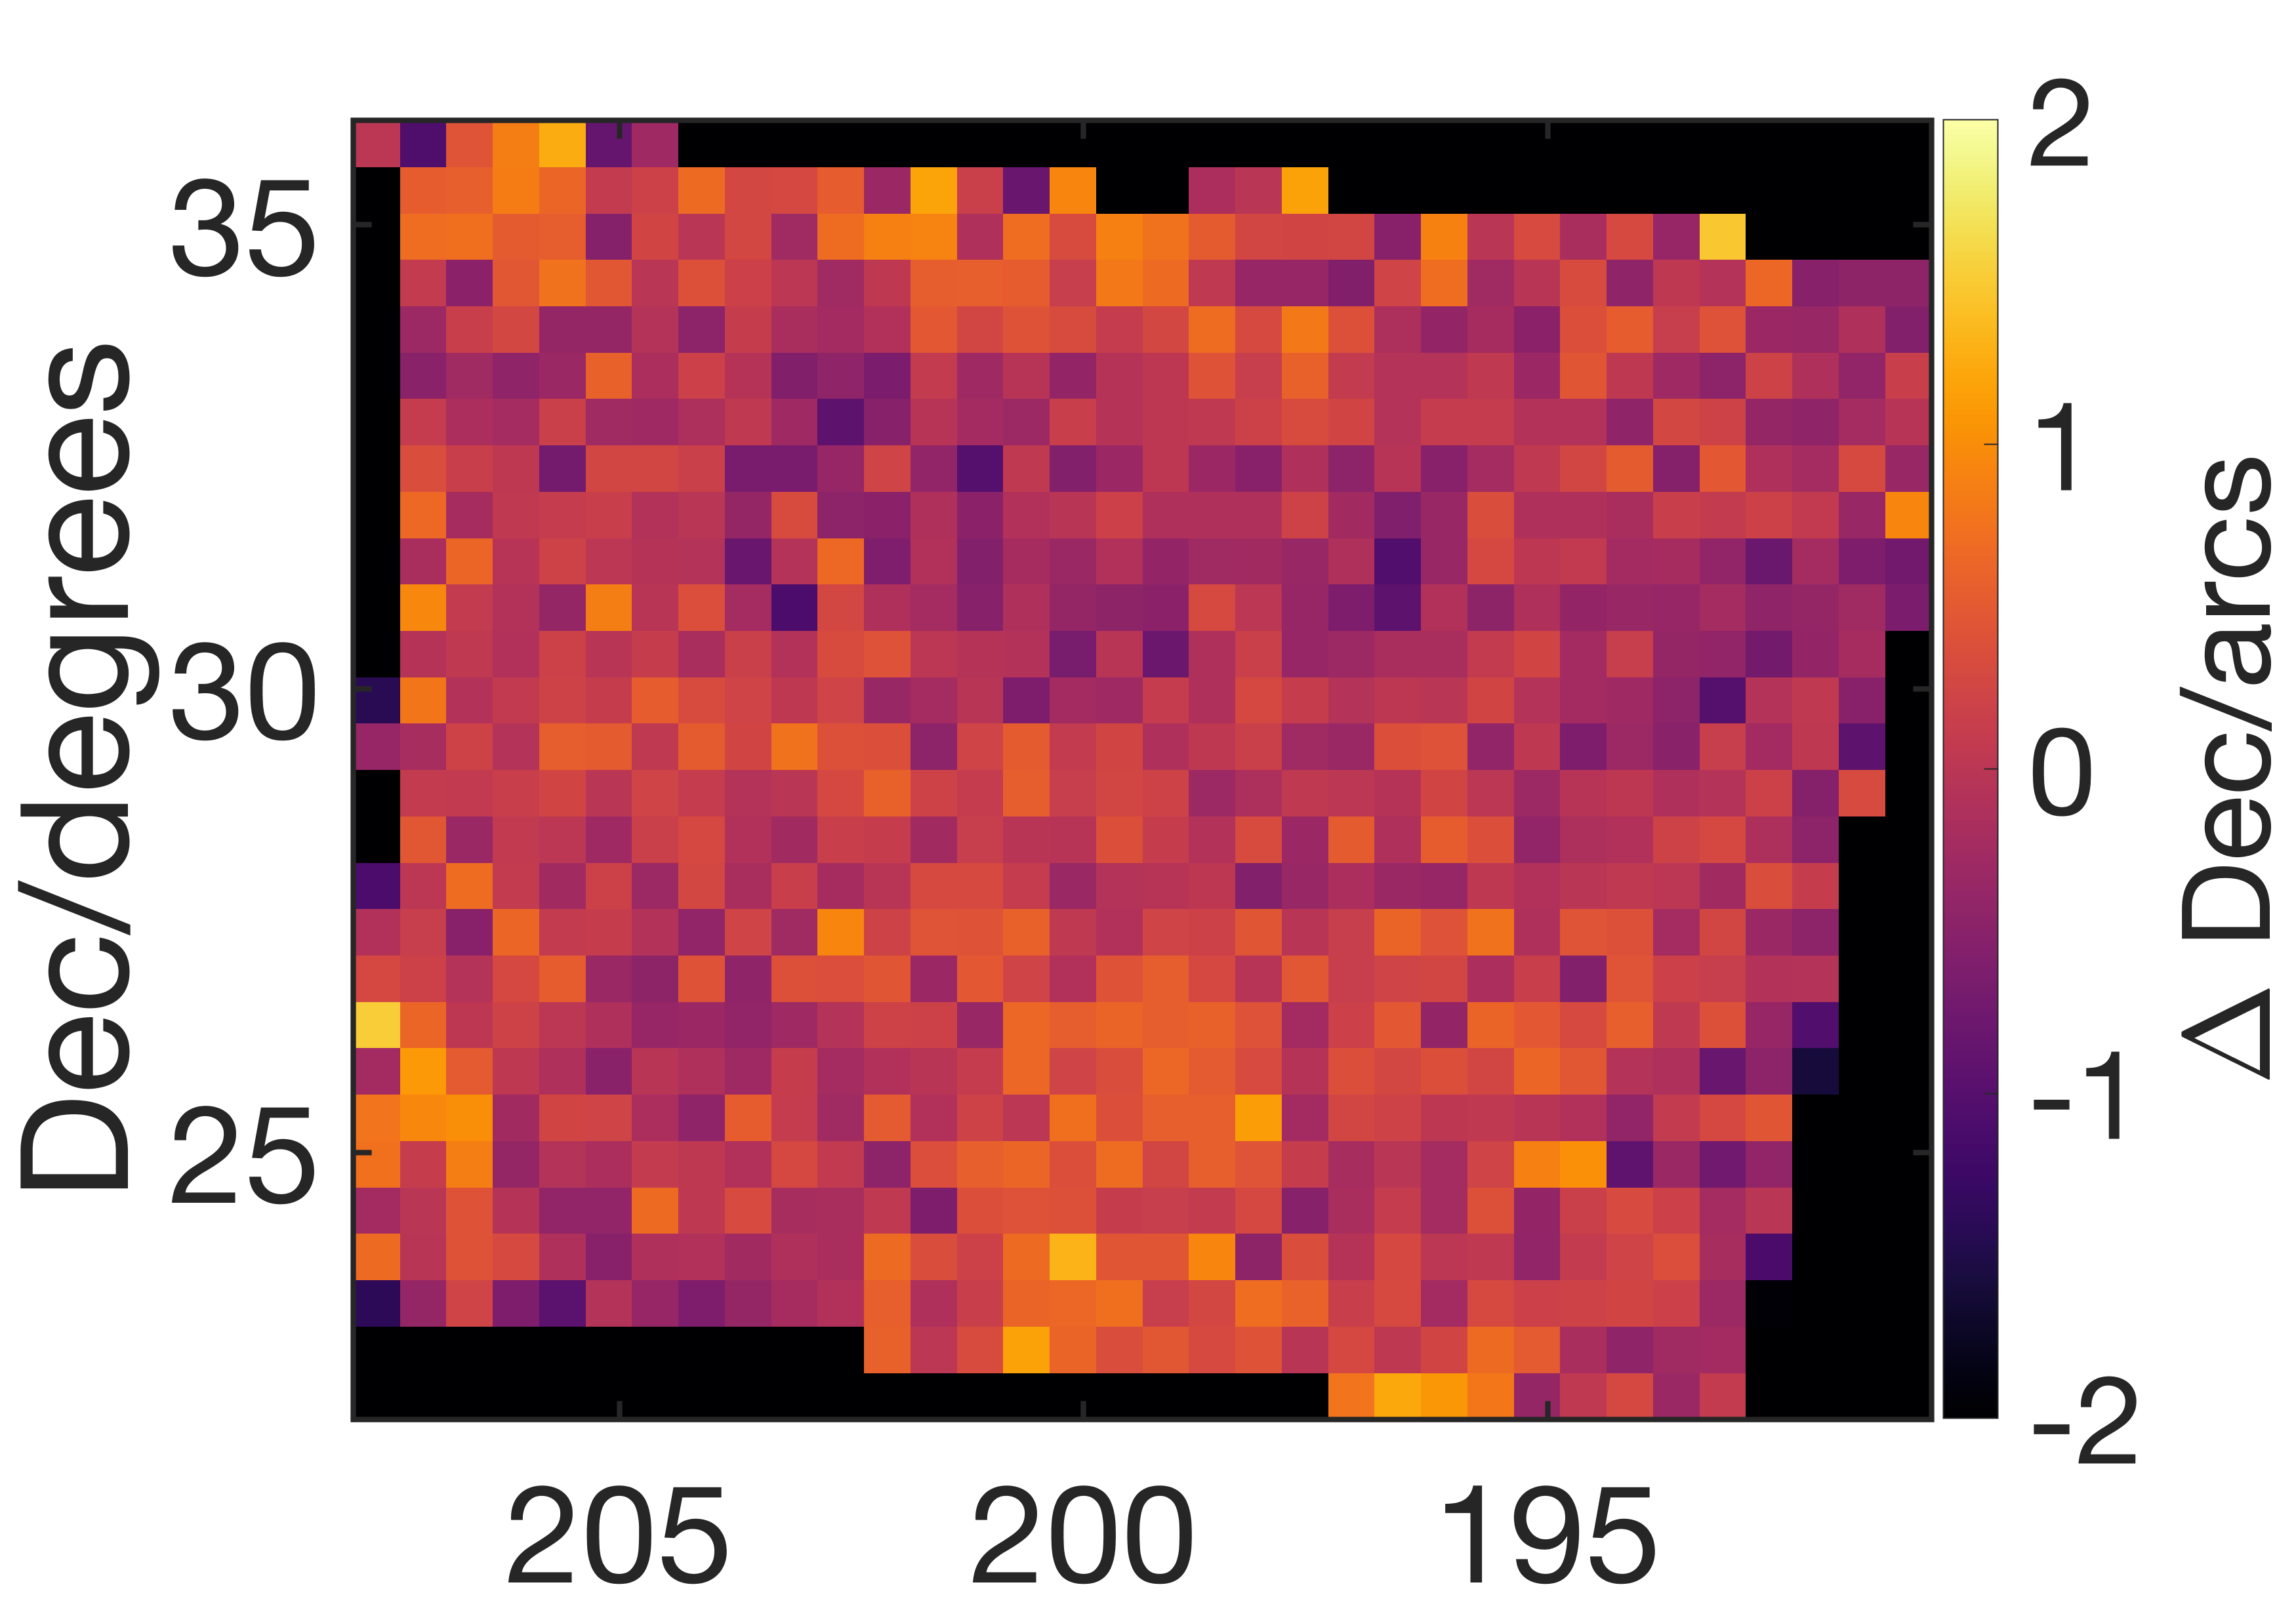
\includegraphics[scale=0.23]{ngp_ddec.png}
\hspace{30mm}\\
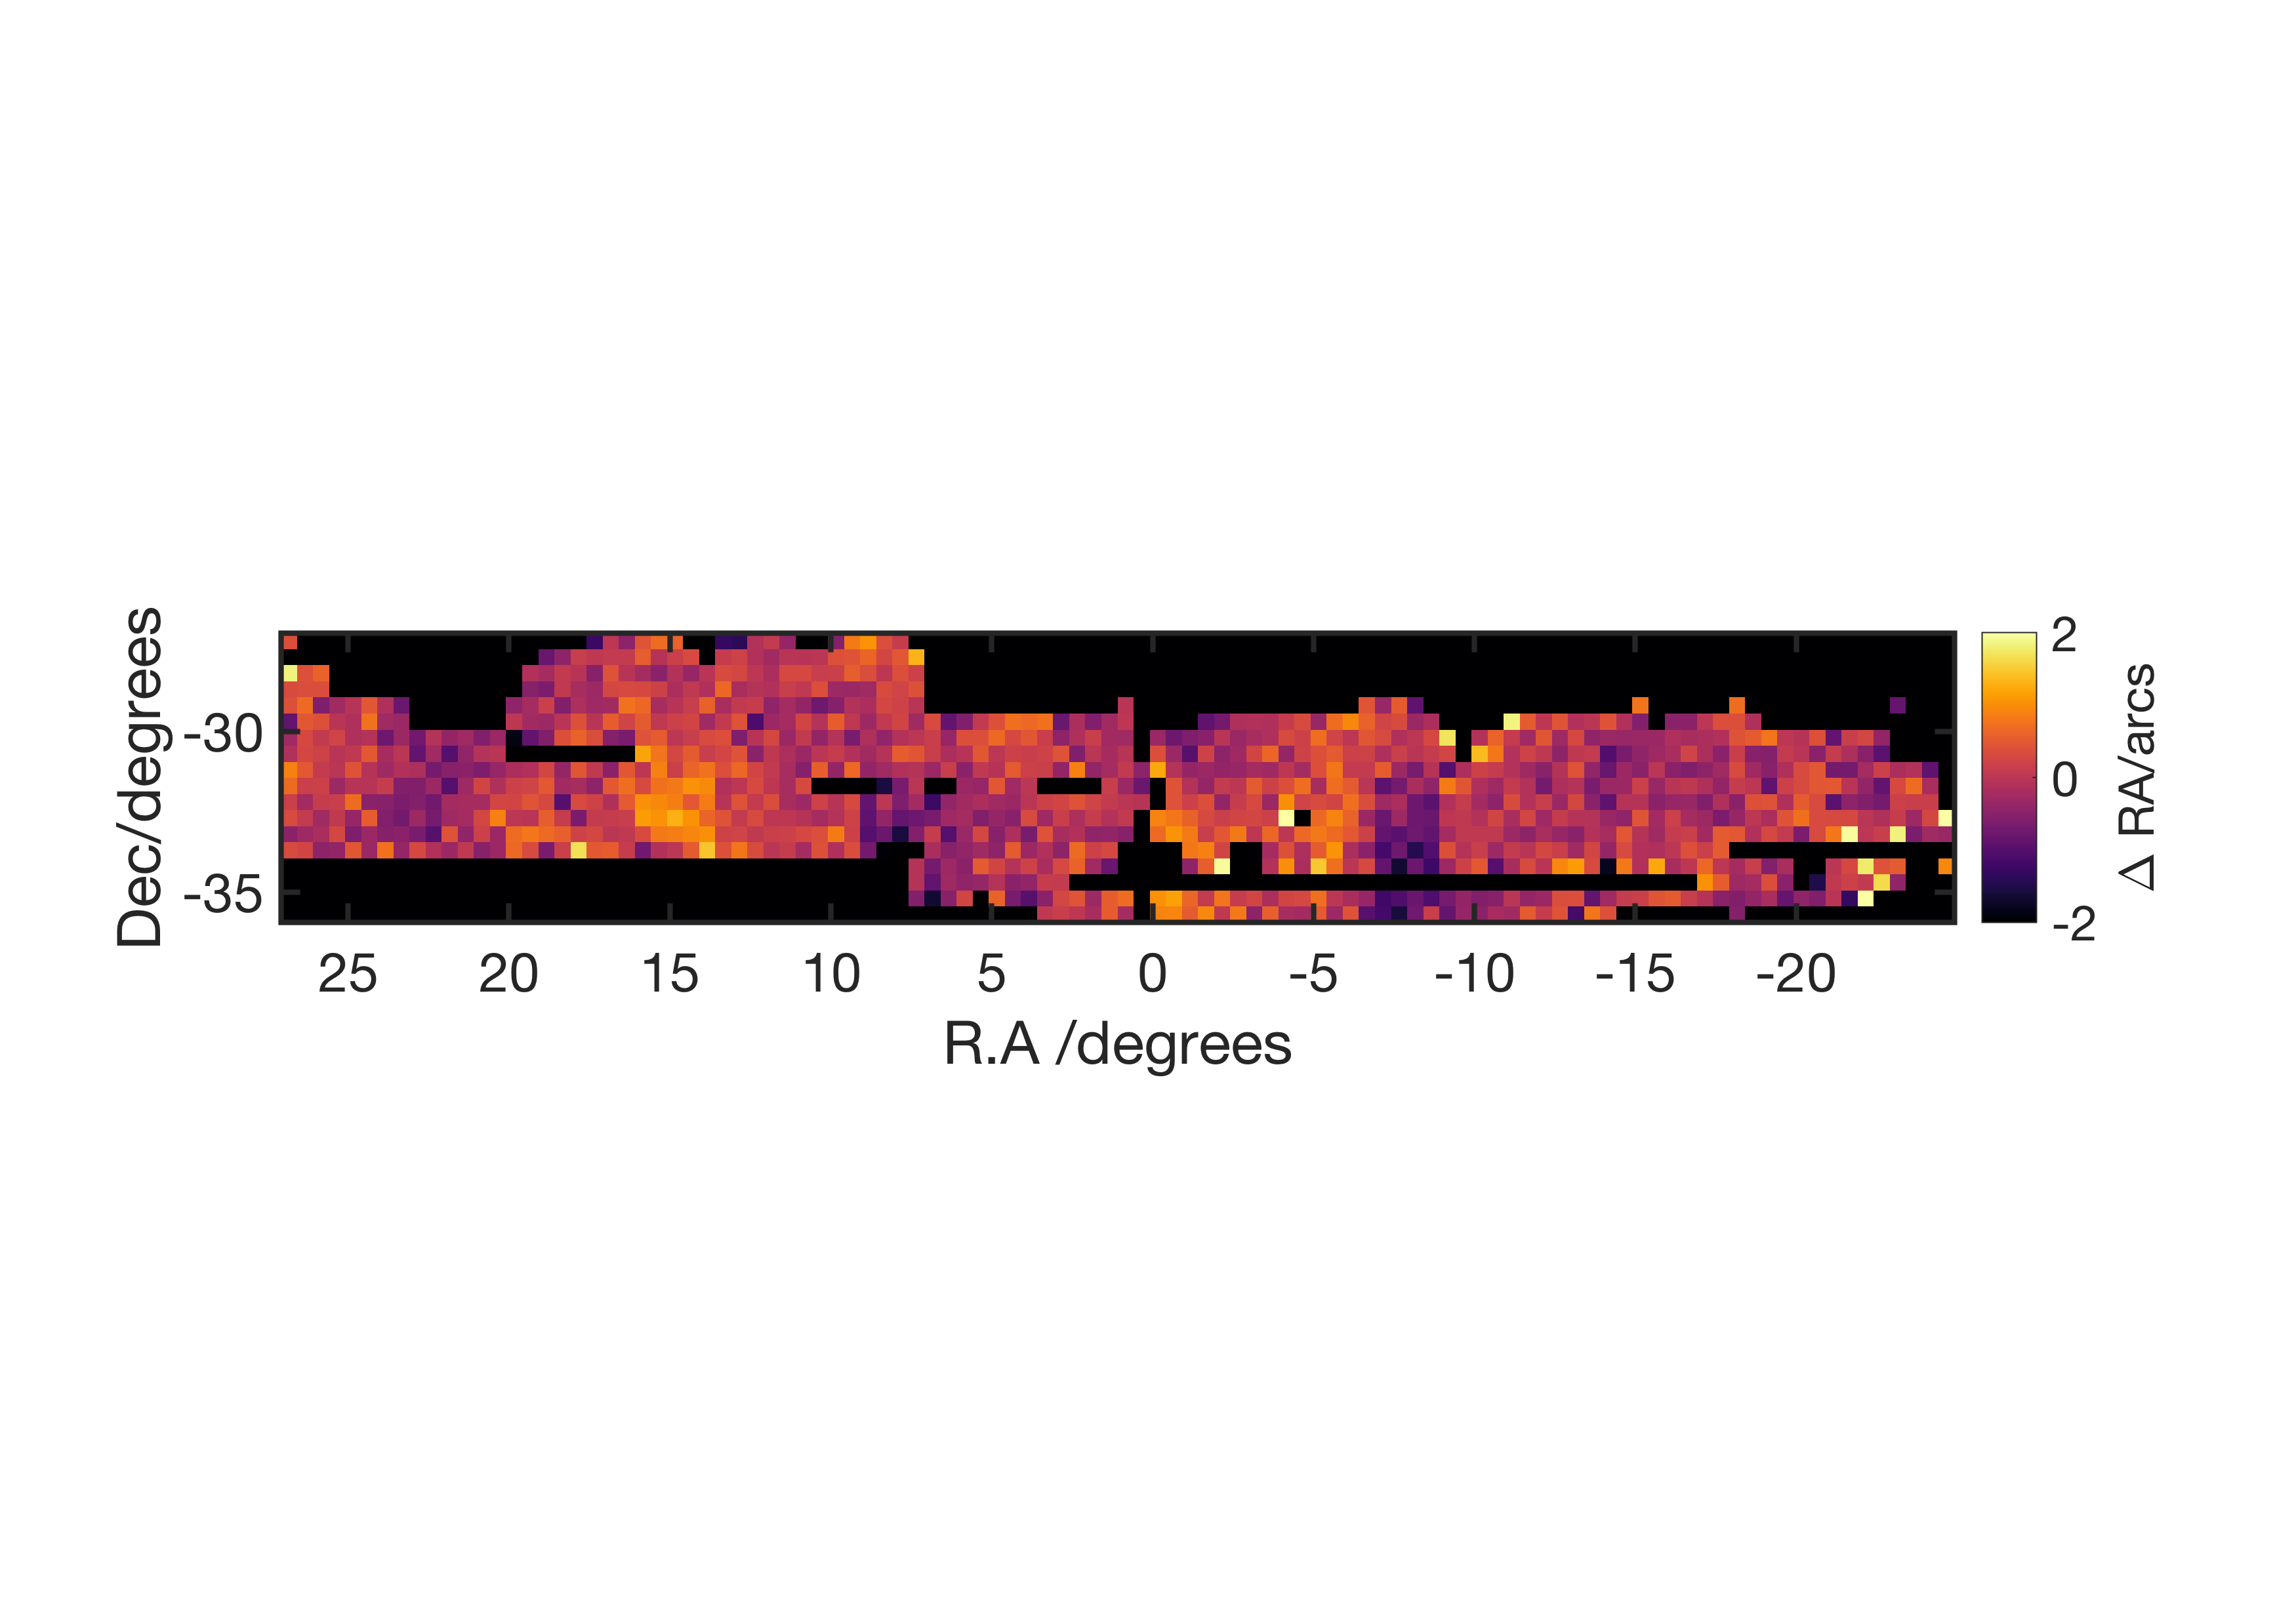
\includegraphics[scale=0.6,trim={0 87mm 0mm 75mm}, clip]{sgp_dra.png}
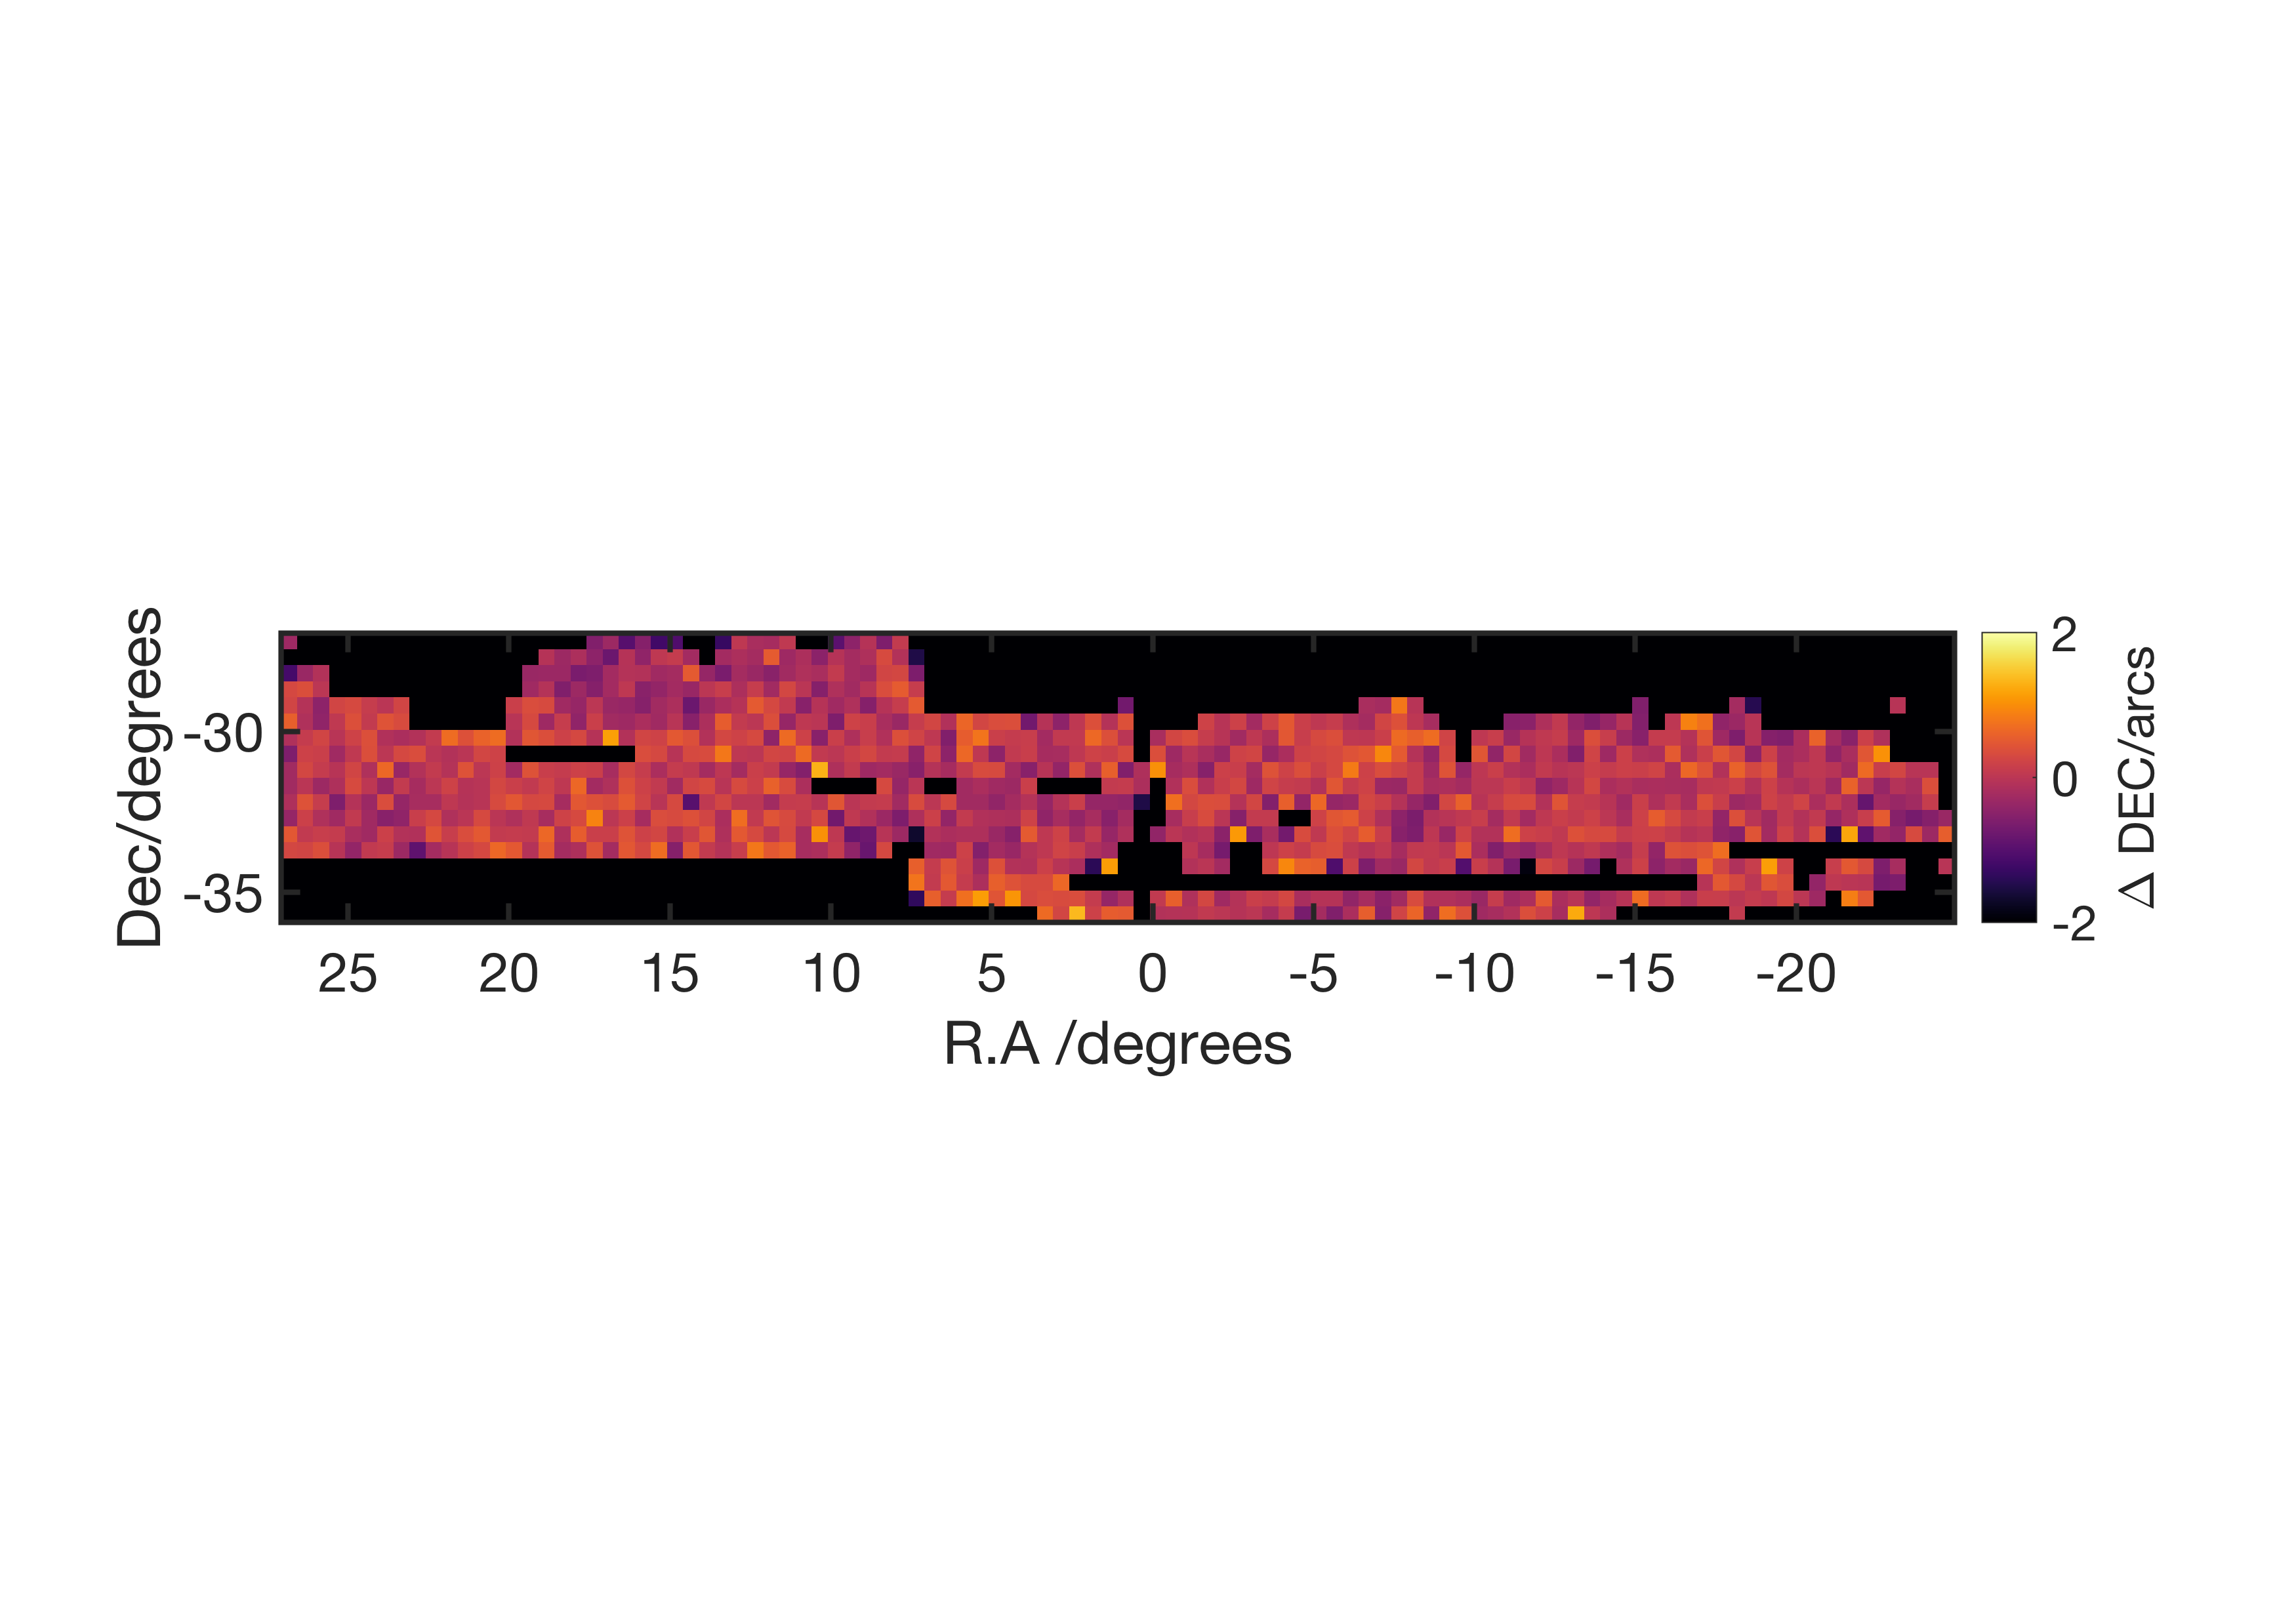
\includegraphics[scale=0.6,trim={0 60mm 0mm 80mm}, clip]{sgp_ddec.png}
\caption{\protect\label{fig_pos_errs} The mean positional errors in
  R.A and Dec. averaged in areas 0.5 deg$\times$0.5deg as a
  function of position on the sky for the NGP and SGP
  fields. 
}
\end{figure*} 

\subsection{Purity, flux boosting and completeness}

Based on Gaussian statistics, we expect $\simeq$0.2\% of the sources
in the catalogue to be spurious. However, V16 argue that this is
likely to be a significant overestimate because our errors, while
being good estimates of the errors on the flux measurements, are
likely to underestimate the signal-to-noise of a detection.

A major problem in submillimetre surveys, where source confusion is
usually an issue, is flux bias or `flux boosting', in which the
measured flux densities are systematically too high. V16 used the
in-out simulations to quantify this effect in the H-ATLAS. Table 6 in
V16 gives estimates of the flux bias as a function of flux density for
all three SPIRE bands. The table shows that at the 4$\sigma$ detection
flux density, the measured flux densities are on average higher than
the true flux densities by $\simeq$20\%, 5\% and 4\% at 250 $\mu$m,
350 $\mu$m and 500 $\mu$m, respectively. Astronomers interested in
comparing the flux densities in the catalogue with the predictions of
models should be aware of this effect. Table 6 in V16 can be used to
correct the flux densities for this effect.

Note that the flux limit for significant PACS detections is much
brighter than the confusion limit, and so PACS fluxes are not affected
by confusion noise. Also the 250-\mic\ noise 
is so much lower than the PACS noise, that the  250-\mic\ selection should
not introduce any significant incompleteness in the PACS sample.
The PACS sample should have completeness and purity as expected for
the quoted Gaussian noise in the flux measurements. 


V16 also used the in-out simulations to estimate the completeness of
the survey as a function of measured flux density in all three SPIRE
bands. This is shown in Figure 21 of V16 and listed in Table 7 of
V16. The completeness at 250\mic is 87\% at the 4$\sigma$
detection limit of the survey.



\section{Summary}

We have described the construction of the source catalogues from the
{\it Herschel} survey of fields around the north and south Galactic
poles. This survey which was carried out in five photometric bands --
100, 160, 250, 350 and 500\mic\ -- was part of the {\it Herschel}
Astrophysical Terahertz Large Area Survey (H-ATLAS), a survey of 660
deg$^2$ of the extragalactic sky. Our source catalogues cover 285
deg$^2$ around the SGP and 170 deg$^2$ around the NGP.

The catalogues contain 118,986 sources for the NGP field and 193.537
sources for the SGP field detected at more than 4$\sigma$ significance
in any of the 250\mic, 350\mic\ or 500\mic\ bands. We present 
photometry in all five bands for each source, including aperture
photometry for sources known to be extended. We discuss all the
practical issues - completeness, reliability, flux boosting, accuracy
of positions, accuracy of flux measurements - necessary to use the
catalogues for astronomical projects.

\section*{Acknowledgments}

PC, LD, HLG, SM and JSM acknowledge support from the European Research
Council (ERC) in the form of Consolidator Grant {\sc CosmicDust}
(ERC-2014-CoG-647939, PI H\,L\,Gomez).  SJM, LD, NB and RJI acknowledge
support from the ERC in the form of the Advanced Investigator Program,
COSMICISM (ERC-2012-ADG 20120216, PI R.J.Ivison).  EV and SAE
acknowledge funding from the UK Science and Technology Facilities
Council consolidated grant ST/K000926/1.  MS and SAE have received
funding from the European Union Seventh Framework Programme
([FP7/2007-2013] [FP7/2007-2011]) under grant agreement No. 607254.

The {\it Herschel}-ATLAS is a project carried out using data from {\it
  Herschel}, which is an ESA space observatory with science
instruments provided by European-led Principal Investigator consortia
and with important participation from NASA.

\begin{thebibliography}{}

%\bibitem[Blain et al.(1993)]{blain93} Blain, A.W. and Longair, M.S. 1993,
%MNRAS, 264, 509

\bibitem[Bourne et al.(2016)]{bourne16} Bourne, N. et al. 2016, MNRAS, 462, 1714

\bibitem[Chapin et al.(2011)]{chap2011} Chapin, E.L. et al. 2011, MNRAS, 411, 505

\bibitem[Dunne et al.(2011)]{dunne2011} Dunne, L. et al. 2011, MNRAS, 417, 1510

\bibitem[Eales et al.(2010)]{eales2010} Eales, S., et al.\ 2010,  \pasp, 122, 499 

\bibitem[Eales et al.(2017)]{eales2017} Eales, S., et al.\ 2017, MNRAS, in press
(arXiv: 1710.01314)

\bibitem[Franceschini et al. (1991)]{franceschini1991} Franceschini,
  A. et al 1991, A\&AS, 89, 285
  
\bibitem[Fudamoto  et al.(2017)]{fud2017} Fudamoto, Y. et al. 2017,
MNRAS, 472, 2028

\bibitem[Furlanetto et al.(2017)]{furl2017} Furlanetto, C. et al. 2017,
MNRAS, submitted (F17; Paper III)

\bibitem[Griffin et al. (2010)]{spire} Griffin, M.J. et al. 2010 A\&A, 518, L3

\bibitem[Griffin et al. (2013)]{griffin2013} Griffin, M.J. et al. 2013,
MNRAS, 434, 992

\bibitem[Ibar et al. (2010)]{pacsmaps} Ibar, E., 2010, MNRAS, 409, 38

\bibitem[Neugebauer et al. (1984)]{neugebauer84} Neugebauer, G. et al. 1984,
ApJ, 278, L1

\bibitem[Pascale et al. (2011)]{spiremaps} Pascale, E., et al. 2011, MNRAS, 415, 911 

\bibitem[Pearson et al. (2013)]{pearson2003} Pearson, E.A. et al. 2013, MNRAS, 435,
2753

\bibitem[\protect\citeauthoryear{{Pilbratt}}{{Pilbratt et al.}}{2010}]{herschel} Pilbratt, G.~L., et al. A\&A, 518, L1

\bibitem[Planck Collaboration XXVI, (2016)]{PlanckXXVI} Planck
  Collaboration XXVI, 2016, A\&A, 594, 26
  
\bibitem[Poglitsch et al. (2010)]{pacs} Poglitsch, A., et al. 2010 A\&A, 518, L2

\bibitem[Rigby et al. (2011)]{rigby2011} Rigby, E.E, et al. 2011, MNRAS, 415, 2336 

\bibitem[Shanks et al. (2015)]{shanks15} Shanks, T. et al. 2015, MNRAS, 451, 4238

\bibitem[(Skrutskie et al. (2006)]{2mass} Skrutskie et al. 2006, AJ 131, 1163
  
\bibitem[Smith et al. (2011)]{Smith11} Smith, D.J.B. et al. 2011, MNRAS, 
416, 857

\bibitem[Smith et al. (2017)]{Smith17} Smith, M.W.L. et al. 2017, ApJ suppl., in press
(S17; Paper I)

\bibitem[Valiante et al. (2016)]{val2016} Valiante, E. et al. 2016, MNRAS, 462, 3146
(V16)

\bibitem[Valtchanov (2017)]{spire17} Valtchanov, I. (Ed.) 2017, The SPIRE Handbook, HERSCHEL-HSC-DOC-0798, v3.1 

\bibitem[Zavala et al. (2017)]{zav2017} Zavala, J.A. et al. 2017, Nature Astronomy,
in press (arXiv: 1707.09022)

\end{thebibliography}
\label{lastpage}

\end{document}

